% -------------------------------
% Plantilla del TFG en la ESIIAB-UCLM. Versión 0.0 (Preliminar)
% Luis de la Ossa
%
% Adaptada para la memoria del trabajo de Procesos de Ingeniería del Software
% (La Grada Colchonera). Se compila con LuaLaTeX (latexmkrc) y también con XeLaTeX.
% -------------------------------
\documentclass[12pt, a4paper]{book}

% -------------------------------
% Información y opciones del documento
% -------------------------------
% -------------------------------
% Plantilla del TFG en la ESIIAB-UCLM. Versión 0.0 (Preliminar)
%
% Luis de la Ossa
% 
% Compilar con XeLaTeX 
% -------------------------------


% -------------------------------
% Comandos comunes
% -------------------------------
\newcommand{\uclm}{Universidad de Castilla-La Mancha\,}
\newcommand{\dsi}{Departamento de Sistemas Informáticos\,}
\newcommand{\esii}{Escuela Superior de Ingeniería Informática de Albacete\,}
\newcommand{\iiia}{Instituto de Investigación en Informática de Albacete\,}


% -------------------------------
% Comandos específicos
% -------------------------------
\newcommand{\autor}{Javier Vela González-Román\,}
\newcommand{\titulo}{Memoria del Proyecto MiApp\,}
%\newcommand{\director}{Nombre del director\,}
%\newcommand{\codirector}{Nombre del codirector\,}
\newcommand{\fecha}{Enero, 2027\,}
 \newcommand{\espec}{Tecnología específica\,} 







% -------------------------------
% Configuración de la plantilla (no tocar) y paquetes añadidos para esta memoria
% -------------------------------
% -------------------------------
% Plantilla del TFG en la ESIIAB-UCLM. Versión 0.0 (Preliminar)
%
% Luis de la Ossa
% 
% Compilar con XeLaTeX 
% -------------------------------


% -------------------------------
% Idioma
% -------------------------------
\usepackage{polyglossia}
\setmainlanguage{spanish}


% -------------------------------
% Fuente
% -------------------------------
% Cualquier tamaño de texto: {\fontsize{100pt}{120pt}\selectfont tutexto}
\usepackage{anyfontsize}
% Selección de fuentes.
\usepackage{fontspec}
% Espacio entre líneas
\usepackage{setspace}
% Fuentes especiales
\usepackage{textcomp,marvosym,pifont}


% -------------------------------
% Otros paquetes de uso común
% -------------------------------
% Símbolos matemáticos
\usepackage{amsmath,amsfonts,amssymb}
% Gráficos
\usepackage{graphicx}
% Posición arbitraria de los gráficos
\usepackage[absolute,overlay]{textpos}
% Apéndices
\usepackage{appendix}


% -------------------------------
% Esquema de colores
% -------------------------------
% Paquete para la definición de colores
\usepackage[table]{xcolor}
% Esquema de colores
% -------------------------------
% Plantilla del TFG en la ESIIAB-UCLM. Versión 0.0 (Preliminar)
%
% Luis de la Ossa
% 
% Compilar con XeLaTeX 
% -------------------------------

% -------------------------------
% Color del tema
% -------------------------------

% Color para los títulos, etc.
%\definecolor{tema}{RGB}{0,0,0}        % Negro 
%\definecolor{tema}{RGB}{182,0,52}     % LOGO UCLM
\definecolor{tema}{RGB}{0,69,134}      % Azul del esquema  
%\definecolor{tema}{RGB}{197,0,11}     % Rojo del esquema     

% Negritas con el color del tema
\newcommand{\bft}[1]{\textcolor{tema}{\bf #1}} 


% -------------------------------
% Esquema de colores
% -------------------------------
% Estos balores coinciden con colores de OpenOffice 
% Se pueden redefinir para que coincidan con las paletas de las 
% herramientas utilizadas para hacer las gráficas.
\definecolor{blanco}{RGB}{255,255,255} 
\definecolor{negro}{RGB}{0,0,0}
\definecolor{gris95}{gray}{.95}
\definecolor{gris75}{gray}{.75}
\definecolor{gris50}{gray}{.50}
\definecolor{gris25}{gray}{.25}
\definecolor{rojo}{RGB}{197,0,11}        % Gráfico 11
\definecolor{azul}{RGB}{0,69,134}        % Gráfico 1
\definecolor{verde}{RGB}{87,157,28}      % Gráfico 4
\definecolor{naranja}{RGB}{255, 149, 14} % Gráfico 10
\definecolor{mostaza}{RGB}{255, 211, 32} % Gráfico 3

% Negrita con color definido 
\newcommand{\bfa}[1]{\textcolor{azul}{\bf #1}} 
\newcommand{\bfr}[1]{\textcolor{rojo}{\bf #1}}
\newcommand{\bfn}[1]{\textcolor{naranja}{\bf #1}}
\newcommand{\bfv}[1]{\textcolor{verde}{\bf #1}}  
\newcommand{\bfm}[1]{\textcolor{mostaza}{\bf #1}} 






% -------------------------------
% Márgenes
% -------------------------------
% Márgenes de las páginas
\usepackage[
  inner	 =	3cm,   % Margen interior
  outer	 =	2.5cm, % Margen exterior
  top	 =	2.5cm, % Margen superior
  bottom =	2.5cm, % Margen inferior
  includeheadfoot, % Incluye cabecera y pie de página en los márgenes
]{geometry}
% Muestra una regla para comprobar el formato de las páginas (descomentar)
%\usepackage[type=upperleft,showframe,marklength=8mm]{fgruler} 


% -------------------------------
% Renombra tablas y bibliografía
% -------------------------------
\addto\captionsspanish{
	\renewcommand{\listtablename}{Índice de tablas} 
	\renewcommand{\tablename}{Tabla}
	\renewcommand{\bibname}{Referencia bibliográfica}
}


% -------------------------------
% Itemize y enumerate. Control de los espacios.
% -------------------------------
\usepackage{enumitem}
\setitemize{itemsep=0pt}
\setenumerate{itemsep=0pt}
\renewcommand{\labelitemi}{\tiny\bft{$\blacksquare$}}
\renewcommand{\labelitemii}{\bft{$\bullet$}}
\renewcommand{\labelitemiii}{\bft{-}}


% -------------------------------
% Enlaces y colores
% -------------------------------
\usepackage{hyperref}
%\hypersetup{
%    colorlinks,
%    citecolor=black,
%    filecolor=black,
%    linkcolor=black,
%    urlcolor=black
%}

% -------------------------------
% Gestión de elementos flotantes
% -------------------------------
% Para forzar a que las figuras aparezcan antes del fin de una sección.
%\usepackage[section]{placeins}

% Gestión de títulos de los elementos flotantes
\usepackage{caption}
% Subfiguras y títulos en subfiguras
\usepackage{subcaption}

% Títulos
\DeclareCaptionFont{tema}{\color{tema}} % Color
\captionsetup{labelfont={tema, bf}}     % Estilo
\captionsetup{font=normalsize}          % Tamaño
\captionsetup{width=.9\linewidth}       % Anchura del título
 % Distancia de la figura al texto.
\setlength{\intextsep}{1cm} 
\setlength{\textfloatsep}{1cm}         
       

% -------------------------------
% Utilidades para tablas
% -------------------------------
% Para fundir filas en tablas
\usepackage{multirow}
% Para definir columnas con ancho fijo y alineación
\usepackage{array,ragged2e}
\newcolumntype{L}[1]{>{\raggedright\let\newline\\\arraybackslash\hspace{0pt}}m{#1}}
\newcolumntype{C}[1]{>{\centering\let\newline\\\arraybackslash\hspace{0pt}}m{#1}}
\newcolumntype{R}[1]{>{\raggedleft\let\newline\\\arraybackslash\hspace{0pt}}m{#1}}


% -------------------------------
% Para tabular
% -------------------------------
\usepackage{tabto}


% -------------------------------
% Formato de títulos, capítulos, etc.
% -------------------------------
\usepackage{titlesec, titletoc}
% Parte
\titleformat{\part}[display]												   	   % Estilo
	{\Huge \centering \color{tema}}                                                % Formato
	{Parte \thepart }                                                              % Etiqueta
	{0.75ex}                                                                       % Separación
	{\bfseries\fontsize{25pt}{40pt}\selectfont}                                    % Entre etiqueta y título            
	[\thispagestyle{empty}]                                                        % Después

% Capítulo		
\titleformat{\chapter}[block]            			 			                    % Estilo  	
	{\vspace{0cm} \flushright \bfseries \LARGE \color{tema}}  	        			% Formato 
	{\thechapter.}                  			  									% Etiqueta
	{0.75ex}                                     									% Separación
	{}                                           									% Entre etiqueta y título
	[\vspace{0.1cm} \rule{0.5\textwidth}{1pt}\vspace*{1cm}\thispagestyle{plain}]    % Después      
  
% Sección
\titleformat{\section}
	{\vspace{5pt}  \Large \color{tema}}
	{\thesection .}
	{0.75ex}
	{}

% Subsección
\titleformat{\subsection}
	{\large \color{tema}}
	{\thesubsection .}
	{0.75ex}
	{}
 
% Subsubsección
\titleformat{\subsubsection}
	{\bf\color{tema}}
	{}
	{0.75ex}
	{}
	 
% Parte (TOC)
\titlecontents{part}[2pc]
  	{\vspace{20pt}\bfseries\filright\Large\color{tema}}
  	{\contentslabel{1.5pc}}{\hspace*{-1.5pc}}
  	{\vspace{5pt}}
  	{}
  
% Capítulo (TOC)
\titlecontents{chapter}[2pc]
  	{\vspace{10pt}\bfseries\large\filright}
  	{\contentslabel{1.5pc}}{\hspace*{-1.5pc}}
  	{\mdseries\titlerule*[0.5pc]{.}\bfseries\contentspage}

% Sección (TOC)
\titlecontents{section}[4pc]
  	{\vspace{5pt}\filright}
  	{\contentslabel{2pc}}{\hspace*{2pc}}
  	{\titlerule*[0.5pc]{.}\contentspage}
  	[\vspace{5pt}]

% Subsección (TOC)
\titlecontents{subsection}[6pc]
  	{\vspace{2.5pt}\filright\small\em}
  	{\contentslabel{3pc}}{\hspace*{-3pc}}
  	{\titlerule*[0.5pc]{.}\contentspage} 
  	
  	
% -------------------------------
% Cabeceras y pie de página
% -------------------------------
\usepackage{fancyhdr}
\pagestyle{fancy}
\fancyhf{}

% Permite incluir la parte. Para ello crea \parttitle
\let\Oldpart\part
\newcommand{\parttitle}{}
\renewcommand{\part}[1]{\Oldpart{#1}\renewcommand{\parttitle}{#1}}

% Cabeceras y pies de página
\fancyhead[LE]{}
\fancyhead[RO]{\slshape \leftmark}
\fancyfoot[LE,RO]{\thepage}
\renewcommand{\footrulewidth}{1pt}
\renewcommand{\headrulewidth}{1pt}
\renewcommand{\chaptermark}[1]{\markboth{#1}{}} % Capítulo (Solo texto)
\renewcommand{\chaptermark}[1]{\markboth{\thechapter. #1}{}} % Capítulo (Número y texto)

% Formato plano para las páginas con títulos (solo incluye el pie de página)
\fancypagestyle{plain}{
\fancyhf{}
\fancyhead{}
\fancyfoot[LE,RO]{\thepage}
\renewcommand{\footrulewidth}{1pt}
\renewcommand{\headrulewidth}{0pt}
}

 
% -------------------------------
% Utilidades
% -------------------------------
% Marcas
\newcommand{\pcite}{\bfr{\large[?]}\,} % Cita pendiente: [?] en rojo y negrita.
\newcommand{\ps}{\bfr{\huge[--}\,} % Pricipio de un bloque en sucio
\newcommand{\fs}{\bfr{\huge--]}\,} % Fin de un bloque en sucio.

% Notas
\usepackage[textsize=tiny,spanish,shadow,textwidth=2cm]{todonotes}

% Para generar textos "random"
\usepackage{lipsum} 
 

% -------------------------------
% Algoritmos y código
% -------------------------------

% Se definen entornos específicos para algoritmos y código que permiten
% gestionar los títulos manera similar en ambos casos, y similar al resto
% de elementos flotantes.
\usepackage{newfloat}

\DeclareFloatingEnvironment[ % Algoritmos
  listname = {Índice de algoritmos},
  name = Algoritmo
]{algorithm}

\DeclareFloatingEnvironment[ % Fragmentos de código
  listname = {Índice de listados de código},
  name = Código
]{code}

% Define un estilo para el encabezado de algoritmos y código.
\DeclareCaptionFormat{algcode}{
% OPCIÓN 1 -> Línea debajo del título
\rule{\dimexpr\textwidth\relax}{0.4pt}\vspace{0cm}
#1#2#3
\vspace{-0.2cm}\rule{\dimexpr\textwidth\relax}{0.4pt} % 
% OPCIÓN 2 -> Sin línea debajo del título
%\rule{\dimexpr\textwidth\relax}{0.4pt}\vspace{0cm}
%#1#2#3
}
\captionsetup[algorithm]{format=algcode, width=\linewidth}
\captionsetup[code]{format=algcode, width=\linewidth}

% Opciones específicas para algoritmos.
\usepackage[noend]{algpseudocode}
% Tamaño de letra y separadores
\makeatletter
\renewcommand{\ALG@beginalgorithmic}{\small\hrule\vskip10pt}
\makeatother
% Variables y funciones
\newcommand{\va}[1]{{\it {#1}}}				
\newcommand{\fu}[1]{{\textsc{#1}}}          
% Palabras clave
\renewcommand{\algorithmicrepeat}{\bft{repetir}}
\renewcommand{\algorithmicuntil}{\bft{hasta}}
\renewcommand{\algorithmicend}{\bft{fin}}
\renewcommand{\algorithmicif}{\bft{si}}
\renewcommand{\algorithmicthen}{\bft{entonces}}
\renewcommand{\algorithmicelse}{\bft{si no}}
\newcommand{\algorithmicelsif}{\algorithmicelse\ \algorithmicif}
\newcommand{\algorithmicendif}{\algorithmicend\ \algorithmicif}
\renewcommand{\algorithmicfor}{\bft{para}}
\renewcommand{\algorithmicforall}{\bft{para cada}}
\renewcommand{\algorithmicwhile}{\bft{mientras}}
\renewcommand{\algorithmicdo}{\bft{hacer}}
\renewcommand{\algorithmicprocedure}{\bft{procedimiento}}
\renewcommand{\algorithmicreturn}{\bft{devolver}}
\renewcommand{\algorithmicfunction}{\bft{función}}
\renewcommand{\algorithmicloop}{\bft{iterar}}

% Opciones específicas para código.
\usepackage{listings}
% Aspecto de los listados de código (ejemplo)
% Los colores se han de cambiar y adaptar a los distintos lenguajes de programación.
\lstset{
    language=Python,
    keywordstyle=\bf\color{tema},  
	breaklines=true,    
	basicstyle={\small\ttfamily},
    tabsize=5,
    frame=t % Es importante no cambiar esta opción (es la línea superior) 
}

% -------------------------------
% Cacacteres pifont de uso común (con color)
% -------------------------------
\newcommand{\vmarkt}{\textcolor{tema}{\ding{52}} }  % Checked (V) Tema
\newcommand{\vmarkr}{\textcolor{rojo}{\ding{52}} }  % Checked (V) Rojo
\newcommand{\vmarka}{\textcolor{azul}{\ding{52}} }  % Checked (V) Azul

\newcommand{\xmarkt}{\textcolor{tema}{\ding{55}} }  % Checked (X) Tema
\newcommand{\xmarkr}{\textcolor{rojo}{\ding{55}} }  % Checked (X) Rojo
\newcommand{\xmarka}{\textcolor{azul}{\ding{55}} }  % Checked (X) Azul

\newcommand{\lmarkt}{\textcolor{tema}{\ding{46}} }  % Lápiz Tema
\newcommand{\lmarkr}{\textcolor{rojo}{\ding{46}} }  % Lápiz Rojo
\newcommand{\lmarka}{\textcolor{azul}{\ding{46}} }  % Lápiz Azul

\newcommand{\hmarkt}{\textcolor{tema}{\ding{43}} }  % Mano Tema
\newcommand{\hmarkr}{\textcolor{rojo}{\ding{43}} }  % Mano Roja 
\newcommand{\hmarka}{\textcolor{azul}{\ding{43}} }  % Mano Azula 

\newcommand{\fmarkt}{\textcolor{tema}{\ding{220}} }  % Flechza Tema
\newcommand{\fmarkr}{\textcolor{rojo}{\ding{220}} }  % Flecha Roja 
\newcommand{\fmarka}{\textcolor{azul}{\ding{220}} }  % Flecha Azul
% -------------------------------
% Paquetes y comandos añadidos para esta memoria.
% Aquí se añade lo que haga falta (TikZ, pgfplots, tablas...) en vez de tocar configuracion.tex.
% -------------------------------

% Utilidades para tablas y texto
\usepackage{booktabs}
\usepackage{csquotes}
\usepackage{icomma}
\usepackage{placeins}

% Diagramas y gráficos
\usepackage{tikz}
\usetikzlibrary{babel,arrows.meta,positioning,shapes.geometric,fit,calc}

\usepackage{pgfplots}
\pgfplotsset{compat=1.18}


\begin{document}

% -------------------------------
% Portada
% -------------------------------
% -------------------------------
% Plantilla del TFG en la ESIIAB-UCLM. Versión 0.0 (Preliminar)
%
% Luis de la Ossa
% 
% Compilar con XeLaTeX 
% -------------------------------
\pagestyle{empty}
\begin{titlepage}\null



\begin{textblock*}{\paperwidth}(0cm,3cm)
\begin{center}

\includegraphics[width=4cm]{figs/logoconciti.png}
\end{center}
\end{textblock*}


\begin{textblock*}{\paperwidth}(0cm,8cm) 
\begin{center}\doublespacing
{\fontsize{16pt}{2pt}\selectfont Universidad de Castilla-La Mancha}

{\fontsize{16pt}{2pt}\selectfont Escuela Superior de Ingeniería Informática}
\end{center}
\end{textblock*}


\begin{textblock*}{\paperwidth}(0cm,12cm) 
\begin{center}\doublespacing 
{\bf\fontsize{18pt}{4pt}\selectfont Trabajo Procesos de Ingeniería Software}

{\fontsize{18pt}{4pt}\selectfont Grado en Ingeniería Informática}

{\fontsize{16pt}{4pt}\selectfont \espec}
\end{center}
\end{textblock*}


% El título ocupa el 80% de la página. Puede adaptarse 
% a la longitud del texto
\begin{textblock*}{0.8\paperwidth}(0.1\paperwidth,17.5cm) 
\begin{center}\doublespacing % onehalfspace
{\bf\fontsize{20pt}{4pt}\selectfont \titulo}

\vskip1cm
{\it \fontsize{18pt}{4pt}\selectfont \autor}
\end{center}
\end{textblock*}


\begin{textblock*}{\paperwidth}(0cm,25.5cm) 
\begin{center}
{\fontsize{14pt}{4pt}\selectfont \fecha}
\end{center}
\end{textblock*}
\end{titlepage}


% -------------------------------
% Fuente del documento (Carlito: libre y con las mismas medidas que Calibri)
% -------------------------------
\setmainfont{Carlito}

% -------------------------------
% Preámbulo: segunda portada, declaración, resumen
% -------------------------------
\frontmatter
% -------------------------------
% Plantilla del TFG en la ESIIAB-UCLM. Versión 0.0 (Preliminar)
%
% Luis de la Ossa
% 
% Compilar con XeLaTeX 
% -------------------------------


% -------------------------------
% Segunda portada
% -------------------------------
\cleardoublepage
\setcounter{page}{1} \null

\begin{textblock*}{3cm}(3cm,2cm) 
\begin{flushleft}

\includegraphics[height=2cm]{figs/logouclm.png}
\end{flushleft}
\end{textblock*}


\begin{textblock*}{2.5cm}(15.95cm,2.45cm) 
\begin{flushright}

\includegraphics[height=1.4cm]{figs/euroinf.jpg}
\end{flushright}
\end{textblock*}

\begin{textblock*}{4cm}(13.5cm,2cm)  % Ancho ajustado a 4cm para evitar overfull hbox
\begin{flushright}

\includegraphics[height=2cm,keepaspectratio]{figs/logoesii.png}
\end{flushright}
\end{textblock*}



\begin{textblock*}{\textwidth}(3cm,8cm) 
\begin{center}\doublespacing 
{\fontsize{14pt}{3pt}\selectfont \bft{TRABAJO DE PROCESOS DE\\ INGENIERÍA DEL SOFTWARE}}

\medskip
{\fontsize{18pt}{4pt}\selectfont Grado en Ingeniería Informática}

\medskip
{\fontsize{16pt}{4pt}\selectfont \espec}
\end{center}
\end{textblock*}


\begin{textblock*}{\textwidth}(3cm,14cm) 
\begin{center}\setstretch{2}
{\fontsize{22pt}{4pt}\selectfont \bft{\titulo}}
\end{center}
\end{textblock*}


\begin{textblock*}{\textwidth}(3cm,20.5cm) 
\begin{flushleft}\doublespacing
{\fontsize{14pt}{4pt}\selectfont \bft{Autor:} \autor}

\ifdefined\director{\fontsize{14pt}{4pt}\selectfont \bft{Tutor:} \director}\fi

\ifdefined\codirector{\fontsize{14pt}{4pt}\selectfont \bft{Co-Tutor:} \codirector}\fi
\end{flushleft}
\end{textblock*}


\begin{textblock*}{\linewidth}(3cm,25cm) 
\begin{flushright}
{\fontsize{14pt}{4pt}\selectfont \fecha}
\end{flushright}
\end{textblock*}


% -------------------------------
% Declaración de autoría
% -------------------------------
\cleardoublepage
\thispagestyle{plain}
\begin{center}
\Large{\bft{Declaración de autoría}}
\end{center}
\vskip1cm

Yo, \autor, declaro que soy el autor del trabajo titulado ``\titulo'', que el citado trabajo no infringe las leyes en vigor sobre propiedad intelectual, y que todo el material no original contenido en dicho trabajo está apropiadamente atribuido a sus legítimos autores, detallándose asimismo el uso responsable de la inteligencia artificial en el Anexo~\ref{anx:ia}.

\vspace*{2cm}
\begin{center}
Albacete, \fecha

\vskip3cm

Fdo.: \autor
\end{center}


% -------------------------------
% Resumen
% -------------------------------
\cleardoublepage
\thispagestyle{plain}
\begin{center}
\Large{\bft{Resumen}}
\end{center}
\vskip1cm

Esta memoria describe el diseño, la implementación y el proceso de desarrollo completo del proyecto \textit{La Grada Colchonera}, una aplicación SaaS organizada en capas con gestión de usuarios y un juego web de tipo \textit{survivor} en pixel art, desarrollado como parte de la asignatura Procesos de Ingeniería del Software (curso 2026-2027). El trabajo abarca dos sprints: el Sprint 1 (29/09–27/10/2026, Hitos 1–4) construye la base SaaS con cuentas, sesión, roles, PostgreSQL, correo, Google OAuth, errores, logs, CI/CD y despliegue en Google Cloud Run; el Sprint 2 (23/10–29/10/2026) implementa la lógica del juego: motor survivor con oleadas, jefes, armas automáticas, mejoras, mundo procedural, club persistente en servidor con validación anti-trampas, logros con historia del Atlético de Madrid, música chiptune y sonidos de grada. Se detalla exhaustivamente la arquitectura en capas, el modelo de datos, la gestión segura de sesiones y contraseñas mediante bcrypt, la metodología Scrum en DoneTonic, GitHub Flow, trazabilidad requisito → PBI → tarea → PR, y la evaluación con 276 pruebas automatizadas y revisión frase a frase contra el enunciado.

\medskip
\noindent\textbf{Palabras clave:} SaaS, Scrum, GitHub Flow, Node.js, PostgreSQL, Google Cloud Run, survivor, pixel art, anti-cheat, Ingeniería del Software.

% -------------------------------
% Abstract
% -------------------------------
\cleardoublepage
\thispagestyle{plain}
\begin{center}
\Large{\bft{Abstract}}
\end{center}
\vskip1cm

This memoir describes the design, implementation, and development process of the \textit{La Grada Colchonera} project, a layered SaaS application with user management and a web \textit{survivor}-style game in pixel art, developed for the Software Engineering Processes course (2026-2027). The work spans two sprints: Sprint 1 (29/09–27/10/2026, Milestones 1–4) builds the SaaS foundation with accounts, sessions, roles, PostgreSQL, email, Google OAuth, error handling, logging, CI/CD, and deployment on Google Cloud Run; Sprint 2 (23/10–29/10/2026) implements the game logic: survivor engine with waves, bosses, automatic weapons, upgrades, procedural world, server-persisted club with anti-cheat validation, achievements tied to Atlético de Madrid history, chiptune music, and crowd sounds. The memoir thoroughly details the layered architecture, data model, secure session and password management with bcrypt, Scrum methodology in DoneTonic, GitHub Flow, requirement → PBI → task → PR traceability, and evaluation with 276 automated tests and phrase-by-phrase review against the specification.

\medskip
\noindent\textbf{Keywords:} SaaS, Scrum, GitHub Flow, Node.js, PostgreSQL, Google Cloud Run, survivor, pixel art, anti-cheat, Software Engineering.


% -------------------------------
% Índices
% -------------------------------
\tableofcontents
\listoffigures
\listoftables
%\listofalgorithms   % Solo si hay algoritmos
%\listofcodes        % Solo si hay listados de código
\cleardoublepage

% -------------------------------
% Capítulos
% -------------------------------
\mainmatter
\pagestyle{fancy}

\chapter{Introducción, Motivación y Objetivos}
\label{cap:introduccion}

% Guía de la plantilla:
% - Motivación: explicar el porqué de este trabajo.
% - Objetivos: objetivo principal y objetivos específicos.
% - Estructura de la memoria: qué contiene cada capítulo y cada anexo.

\section{Motivación}
\lipsum[1]

\section{Objetivos}
\lipsum[2]

\section{Estructura de la memoria}
\lipsum[3]

% \chapter{Antecedentes}

% La plantilla indica que no es necesario en este trabajo (sí en el TFG).
% No se incluye en Memoria.tex.
   % La plantilla indica que no es necesario en este trabajo
\chapter{Propuesta de Solución, Metodología y Herramientas}
\label{cap:propuesta}

\section{Propuesta de solución}

La propuesta de solución responde a la necesidad de construir una base sólida para una plataforma SaaS comunitaria con capacidad de ampliación futura. Antes de abordar las particularidades de implementación o la elección concreta de librerías, la solución se concibe como un sistema distribuido estructurado bajo el principio de separación de responsabilidades en tres capas fundamentales: una capa de interfaz de usuario con navegación ligera, una capa intermedia que encapsula las reglas de negocio y políticas de autorización, y una capa de persistencia encargada de conservar el estado del sistema.

En el plano funcional, la solución propone un mecanismo de autenticación en el que los usuarios pueden registrarse y acceder al servicio de forma segura, garantizando la preservación de la sesión durante su navegación mediante identificadores almacenados en el servidor. Asimismo, se plantea un modelo de autorización diferenciado que distinga a los usuarios estándar de aquellos con privilegios administrativos. Los administradores disponen de visibilidad global sobre las cuentas existentes y ostentan la capacidad de revocar accesos, mientras que los usuarios conservan el control para solicitar su propia baja del sistema. Para asegurar una experiencia coherente, la solución postula que ninguna decisión de seguridad ni comprobación de permisos dependa exclusivamente de la interfaz del cliente: cualquier petición debe ser rigurosamente validada en el servidor antes de modificar el estado persistente.

\section{Metodología}

Para articular el desarrollo y garantizar la transparencia del progreso, se adoptó el marco de trabajo ágil Scrum \cite{scrumguide}, adaptado a las condiciones de un proyecto individual de ingeniería del software.

\subsection{Gestión con Scrum en DoneTonic}

La planificación y seguimiento del proyecto se centralizaron en la plataforma DoneTonic, dentro del espacio de trabajo \textit{TFG} y el proyecto \textit{Colchoneros}. El ciclo de trabajo corresponde al denominado \textbf{Sprint 1}, planificado entre el 29/09/2026 y el 27/10/2026.

A partir del análisis detallado del enunciado de la asignatura \cite{enunciado}, se elaboró un \textit{Product Backlog} compuesto por 19 elementos de la lista de producto (PBIs, numerados de P1 a P19), desglosados en un total de 32 tareas técnicas (T1 a T32). Puesto que todos los requisitos recogidos en el enunciado poseen carácter prescriptivo para la evaluación del software, la totalidad de los PBIs se catalogó con prioridad obligatoria (\textit{MUST}).

Para velar por la integridad técnica del producto se definió una estricta Definición de Hecho (\textit{Definition of Done}, DoD). Se consideró que una tarea técnica estaba completada exclusivamente cuando satisfacía los siguientes cuatro criterios concurrentes:
\begin{enumerate}
    \item El código fuente reside en su rama de trabajo específica y se vincula formalmente a un pull request que referencia la tarea.
    \item Todas las pruebas automatizadas superan satisfactoriamente la validación en el entorno de integración continua (verificación del check \textit{Pruebas}).
    \item El pull request correspondiente ha sido revisado y fusionado en la rama de integración del hito.
    \item La documentación de soporte (como guías de despliegue o ficheros de configuración de ejemplo) ha sido actualizada coherentemente si la tarea lo requería.
\end{enumerate}

Por su parte, un hito del sprint se considera completado cuando su rama integradora se ha fusionado en la rama principal, el software se encuentra desplegado de forma operativa en la nube y se ha emitido la correspondiente etiqueta de versión (\textit{release}).

\subsection{Flujo de versiones: GitHub Flow adaptado}

El desarrollo colaborativo y la gestión del código fuente siguieron las directrices de GitHub Flow \cite{githubflow}, estructuradas de forma jerárquica para reflejar los hitos pedagógicos:
\begin{itemize}
    \item \textbf{Rama principal (\texttt{main}):} Representa en todo momento el código estable y listo para producción. Se encuentra protegida en GitHub, imposibilitando modificaciones directas y exigiendo obligatoriamente la resolución favorable del pipeline de integración continua.
    \item \textbf{Ramas de integración de hito (\texttt{hito-N/integracion}):} Actúan como puntos de convergencia para el conjunto de tareas pertenecientes a un mismo bloque temático semanal antes de su incorporación definitiva a la rama principal.
    \item \textbf{Ramas de tarea (\texttt{hito-N/Tx-descripcion}):} Creadas a partir de la rama de integración correspondiente para acometer de forma aislada una única tarea del backlog.
\end{itemize}

El ciclo operativo de cada cambio se rigió por las normas estipuladas en la guía de contribución del repositorio:
\begin{enumerate}
    \item Selección de la tarea \texttt{Tx} en el tablero de DoneTonic y creación de la rama técnica asociada.
    \item Generación de commits con mensajes descriptivos en tiempo imperativo y prefijo identificativo (por ejemplo, \texttt{[Tx] Descripción del cambio}).
    \item Ejecución local de la batería de pruebas unitarias y de integración (\texttt{npm test}) previo a la publicación de cambios.
    \item Apertura de un pull request hacia la rama de integración del hito y verificación del paso exitoso del CI en GitHub Actions.
    \item Fusión del pull request y transición automática de la tarea a estado \textit{HECHO} en el tablero ágil.
\end{enumerate}

\section{Herramientas}

Para sustentar las distintas dimensiones del proyecto se seleccionó un conjunto de herramientas y tecnologías de acuerdo con los requisitos técnicos exigidos en la asignatura. La Tabla \ref{tab:herramientas} sintetiza las herramientas empleadas, estructuradas según su ámbito de aplicación en el ciclo de vida del software.

\begin{table}[htbp]
\centering
\small
\begin{tabular}{L{3cm} L{3.2cm} L{7.2cm}}
\toprule
\textbf{Categoría} & \textbf{Herramienta / Tecnología} & \textbf{Propósito en el proyecto} \\
\midrule
\multirow{2}{*}{\textbf{Gestión ágil}} 
    & DoneTonic & Gestión del backlog, asignación de PBIs y tareas en tablero Kanban, y seguimiento del burndown del sprint \cite{scrumguide}. \\
    & GitHub Projects / PRs & Trazabilidad de cambios, control de ramas protegidas y revisión colaborativa de código \cite{githubflow}. \\
\midrule
\multirow{4}{*}{\textbf{Desarrollo}} 
    & Node.js 22 & Entorno de ejecución en servidor para unificar JavaScript en backend y frontend \cite{nodejs}. \\
    & Express 5 & Framework web minimalista para articular la capa API y gestionar errores asíncronos \cite{express}. \\
    & PostgreSQL (Neon) & Sistema gestor de bases de datos relacional serverless con capa gratuita en nube \cite{postgresql,neonlimits}. \\
    & Playwright & Automatización de navegador para generar capturas de interfaz homogéneas. \\
\midrule
\multirow{3}{*}{\textbf{Despliegue y CI/CD}} 
    & GitHub Actions & Automatización del pipeline de pruebas continuas, construcción Docker y entrega \cite{githubactions}. \\
    & Google Cloud Run & Plataforma PaaS de contenedores con autoescalado para el despliegue principal \cite{cloudrun}. \\
    & Render & Plataforma en la nube utilizada como proveedor alternativo de despliegue continuo. \\
\midrule
\multirow{2}{*}{\textbf{Documentación y soporte}} 
    & LuaLaTeX & Motor tipográfico para la composición y maquetación de la memoria técnica del proyecto. \\
    & Claude (Cowork) & Asistente inteligente utilizado en la preparación de código, artefactos y documentación técnica. \\
\bottomrule
\end{tabular}
\caption{Clasificación de herramientas empleadas en el proyecto.}
\label{tab:herramientas}
\end{table}

La combinación de estas herramientas permitió orquestar un entorno homogéneo y plenamente automatizado, reduciendo al mínimo las dependencias manuales y proporcionando trazabilidad absoluta desde la definición de requisitos hasta la verificación del despliegue en producción.

\chapter{Descripción de la Aplicación}
\label{cap:descripcion}

Este capítulo detalla la especificación y diseño del sistema software desarrollado en \textit{La Grada Colchonera}, una plataforma SaaS web orientada a la afición rojiblanca construida como proyecto de aficionado sin vinculación formal con el Club Atlético de Madrid. El sistema conjuga un núcleo de servicios web para la gestión de identidades y persistencia con un videojuego web determinista de supervivencia en tiempo real (\textit{survivor}), cuyas mecánicas completas se describen en profundidad en el Capítulo~\ref{cap:juego}. A continuación se presentan el catálogo integral de requisitos, la arquitectura general del sistema, las decisiones de diseño adoptadas, el modelo de datos relacional, la especificación de interfaces API, los diagramas de secuencia de los flujos principales, el análisis de seguridad y el manual de uso del subsistema SaaS.

\section{Requisitos del sistema}

El proyecto integra dos conjuntos complementarios de requisitos funcionales: los correspondientes a la plataforma SaaS básica definidos en las prescripciones de la asignatura \cite{enunciado} y abordados durante el Sprint 1 (Hitos 1 a 4), y los relativos a la lógica jugable implementados a lo largo del Sprint 2. Asimismo, se define un compendio de requisitos no funcionales que rigen la calidad, seguridad y mantenibilidad de la solución.

La Tabla~\ref{tab:rf-sprint1} recopila los requisitos funcionales de la plataforma base (RF-01 a RF-13). La Tabla~\ref{tab:rj-sprint2} cataloga los requisitos funcionales específicos del videojuego (RJ-01 a RJ-20). Por su parte, la Tabla~\ref{tab:rnf} enumera los requisitos no funcionales (RNF-01 a RNF-12). Para cada requisito se indica el elemento del Product Backlog (PBI) asociado y el módulo o fichero representativo donde se materializa.

\begin{longtable}{@{}L{1.4cm} L{7.1cm} L{1.2cm} L{4.8cm}@{}}
\caption{Requisitos funcionales del Sprint 1 (Hitos 1--4).}\label{tab:rf-sprint1}\\
\toprule
\textbf{Id} & \textbf{Requisito} & \textbf{PBI} & \textbf{Dónde se cumple} \\ \midrule \endfirsthead
\toprule
\textbf{Id} & \textbf{Requisito} & \textbf{PBI} & \textbf{Dónde se cumple} \\ \midrule \endhead
RF-01 & Registro local con correo y contraseña (formato válido, unicidad y clave de al menos 8 caracteres). & P8 & \texttt{userService.register}, \texttt{POST /api/auth/register}, vista \texttt{registro.js}. \\
RF-02 & Inicio de sesión local con respuesta opaca unificada ante correo inexistente o contraseña incorrecta. & P8 & \texttt{userService.authenticate}, \texttt{POST /api/auth/login}. \\
RF-03 & Mantenimiento de sesión al recargar y revocación en servidor vinculada a base de datos. & P9 & \texttt{express-session}, tabla \texttt{session}, \texttt{GET /api/auth/me}, \texttt{POST /api/auth/logout}. \\
RF-04 & Protección de rutas en el servidor denegando peticiones sin sesión activa (código HTTP 401). & P10 & Middleware \texttt{requireAuth}. \\
RF-05 & Persistencia relacional de datos en motor PostgreSQL. & P11 & PostgreSQL (Neon), \texttt{postgresUserRepository}, migraciones versionadas. \\
RF-06 & Control de acceso basado en roles (\textit{user} y \textit{admin}) con bootstrap de un primer administrador. & P13 & Middlewares \texttt{requireRole}, \texttt{requireSelfOrRole}, \texttt{userService.ensureAdmin}. \\
RF-07 & Listado de usuarios, consulta de actividad y modificación de roles reservada a administradores. & P13 & \texttt{GET /api/users}, \texttt{GET /api/users/:id/active}, \texttt{PATCH /api/users/:id/role}, vista \texttt{admin.js}. \\
RF-08 & Baja voluntaria y eliminación administrativa de cuentas; preservación del último administrador; liberación de credenciales. & P13 & \texttt{DELETE /api/users/:id} (baja lógica), vistas \texttt{perfil.js} y \texttt{admin.js}. \\
RF-09 & Registro estructurado en trazas JSON de eventos relevantes de seguridad y ciclo de vida. & P14 & \texttt{src/logger.js}, middleware \texttt{requestLogger}. \\
RF-10 & Confirmación obligatoria de cuenta mediante correo transaccional y reenvío de enlaces. & P16 & \texttt{accountConfirmationService}, \texttt{tokenSigner}, \texttt{mailer}, \texttt{GET /api/auth/confirm}. \\
RF-11 & Inicio de sesión federado mediante Google OAuth 2.0 y vinculación segura de cuentas. & P15 & \texttt{googleOAuth.js}, \texttt{GET /api/auth/google}, \texttt{userService.loginWithOAuth}. \\
RF-12 & Tratamiento homogéneo de errores sin exposición de información interna ni trazas técnicas. & P17 & \texttt{errorHandler.js}, componentes \texttt{avisos.js}, cliente \texttt{api.js}. \\
RF-13 & Prueba técnica de admisión restrictiva por dominios de correo electrónico autorizados. & — & \texttt{domainPolicy.js}, \texttt{POST /api/prueba/dominio}. \\
\bottomrule
\end{longtable}

\begin{longtable}{@{}L{1.4cm} L{7.1cm} L{1.2cm} L{4.8cm}@{}}
\caption{Requisitos funcionales del juego (Sprint 2).}\label{tab:rj-sprint2}\\
\toprule
\textbf{Id} & \textbf{Requisito} & \textbf{PBI} & \textbf{Dónde se cumple} \\ \midrule \endfirsthead
\toprule
\textbf{Id} & \textbf{Requisito} & \textbf{PBI} & \textbf{Dónde se cumple} \\ \midrule \endhead
RJ-01 & Acceso restringido al menú del juego a usuarios autenticados; asociación de progresos a la cuenta. & P20, P29 & \texttt{ui.js} (ruta \texttt{\#/jugar}), \texttt{requireAuth} en \texttt{/api/juego}, tablas \texttt{juego\_perfiles} y \texttt{juego\_records}. \\
RJ-02 & Simulación survivor continua con oleadas automáticas, orbes de experiencia, subida de nivel y dificultad incremental. & P21, P24, P34 & \texttt{mundo.js}, \texttt{oleadas.js}, \texttt{mejoras.js}, \texttt{config.js}. \\
RJ-03 & Renderizado gráfico en pixel art generado por código y proyección de cámara en tres cuartos. & P22, P45 & \texttt{sprites.js}, \texttt{render.js}, \texttt{render-mundo.js}. \\
RJ-04 & Selección de 36 futbolistas en 4 posiciones y 2 entrenadores tácticos con habilidad definitiva (\textit{ulti}). & P23, P38 & Módulos de Vestuario y Dirección (\texttt{juego.js}), \texttt{config.js}, \texttt{ulti.js}. \\
RJ-05 & Armas de disparo automático con 5 niveles de progresión, habilidades pasivas y bloqueo temporal por minuto de juego. & P24, P39 & \texttt{armas.js}, \texttt{mejoras.js}, \texttt{combate.js}. \\
RJ-06 & 16 clubes rivales con patrones de comportamiento diferenciados (embestida, disparo a distancia, rodeo de obstáculos y élites). & P25 & \texttt{rivales.js}, \texttt{oleadas.js}. \\
RJ-07 & 10 jefes mayores con tres fases de combate, advertencias visuales de ataque, escolta y jugada estrella final. & P26, P46 & \texttt{jefes.js}, \texttt{oleadas.js}. \\
RJ-08 & Escenario procedural continuo con colisiones macizas, gradas, lluvia, barro y mesetas transitables. & P27, P35, P41 & \texttt{terreno.js}, \texttt{mundo.js}. \\
RJ-09 & Ambientación ambiental evolutiva con 5 finales históricas que alternan iluminación y cánticos cada cinco minutos. & P36 & \texttt{config.js}, \texttt{render-mundo.js}, \texttt{musica.js}. \\
RJ-10 & Control mediante teclado, ratón y joystick táctil; interfaz con pausa, pantalla completa y configuración de volumen. & P28 & \texttt{entrada.js}, \texttt{ajustes.js}, \texttt{juego.js}. \\
RJ-11 & Persistencia del club en servidor y verificación anti-trampas de las estadísticas declaradas al finalizar la partida. & P29 & \texttt{juegoService.finalizarPartida}, migración \texttt{003}. \\
RJ-12 & Contratación de futbolistas mediante fichas obtenidas al derrotar jefes, con probabilidades según rareza histórica. & P30, P38 & \texttt{club.js}, \texttt{POST /api/juego/contratar}, vista \texttt{firma.js}. \\
RJ-13 & Sistema de entrenamiento de atributos básicos financiado mediante puntos obtenidos por bajas y victorias. & P31 & \texttt{club.js}, \texttt{POST /api/juego/entrenar}. \\
RJ-14 & Tabla de clasificación comunitaria anonimizada (mostrando exclusivamente mote y avatar de cada aficionado). & P32 & Tabla \texttt{juego\_records}, \texttt{GET /api/juego/ranking}. \\
RJ-15 & 24 combinaciones tácticas y 6 poderes ULTRAS desbloqueables al maximizar sinergias concretas. & P33, P40 & \texttt{ultras.js}, \texttt{render-ultras.js}, vista Combinaciones. \\
RJ-16 & Modo de pruebas reservado para perfiles administradores que permite desbloquear inventarios y forzar escenarios. & P34 & \texttt{POST /api/juego/desbloquear}, \texttt{scripts/desbloquear-juego.js}. \\
RJ-17 & Configuración de mote único y avatar personalizado integrados en cabecera, perfil y clasificación. & P37 & \texttt{PUT /api/juego/identidad}, migración \texttt{004}. \\
RJ-18 & 29 logros conmemorativos de la historia del club validados en servidor que habilitan 10 equipaciones alternativas. & P42 & \texttt{logros.js}, \texttt{juegoService}. \\
RJ-19 & Pantalla de desenlace con cómputo pormenorizado de bajas, tiempo resistido, daño por habilidad y recompensas. & P43 & \texttt{fin-ui.js}, \texttt{combate.js}. \\
RJ-20 & Paisaje sonoro compuesto por melodías chiptune, efectos de impacto y murmullo ambiental sintetizados con Web Audio. & P44 & \texttt{audio.js}, \texttt{musica.js}, \texttt{ajustes.js}. \\
\bottomrule
\end{longtable}

\begin{longtable}{@{}L{1.5cm} L{5.2cm} L{7.8cm}@{}}
\caption{Requisitos no funcionales del sistema.}\label{tab:rnf}\\
\toprule
\textbf{Id} & \textbf{Requisito} & \textbf{Cómo se cumple} \\ \midrule \endfirsthead
\toprule
\textbf{Id} & \textbf{Requisito} & \textbf{Cómo se cumple} \\ \midrule \endhead
RNF-01 & Seguridad de credenciales y sesiones & Cifrado de contraseñas mediante \texttt{bcrypt} (coste 10) \cite{bcrypt}, cookies con atributos \texttt{httpOnly}, \texttt{secure} y \texttt{sameSite=lax}, regeneración de identificadores de sesión en login y parametrización total de sentencias SQL. \\
RNF-02 & Gestión segura de secretos & Variables de entorno en desarrollo e inyección desde Google Secret Manager en producción; validación estricta al arranque impidiendo el inicio si faltan claves obligatorias. \\
RNF-03 & Arquitectura modular y desacoplamiento & Separación estricta de responsabilidades en capas (presentación, API, servicios, repositorios e integraciones) aplicando el patrón de inyección de dependencias. \\
RNF-04 & Verificación automatizada e integración continua & 276 pruebas ejecutadas nativamente con \texttt{node:test}; bloqueo de ramas protegidas en GitHub ante fallos del CI. \\
RNF-05 & Despliegue continuo automatizado & Entrega desatendida en Google Cloud Run y Render sin intervención manual tras superar las pruebas en \texttt{main}. \\
RNF-06 & Alta disponibilidad y control de costes & Arquitectura sin servidor (\textit{serverless}) con escalado a cero en capas de uso gratuito y créditos educativos. \\
RNF-07 & Accesibilidad web & Marcado semántico HTML5, gestión programática del foco en navegación SPA, regiones \texttt{aria-live} para avisos dinámicos, soporte completo de teclado y respeto a la preferencia \texttt{prefers-reduced-motion}. \\
RNF-08 & Adaptabilidad responsive & Interfaz adaptada a dispositivos móviles; transformación del panel de administración a tarjetas y simulación de joystick táctil virtual en el juego. \\
RNF-09 & Rendimiento del motor de simulación & Mantenimiento estable de 60 fotogramas por segundo mediante bucle de paso fijo, particionado espacial por celdas para colisiones y caché de texturas procedurales. \\
RNF-10 & Trazabilidad formal del ciclo de vida & Correspondencia biunívoca requisito $\rightarrow$ PBI $\rightarrow$ tarea $\rightarrow$ rama $\rightarrow$ pull request $\rightarrow$ versión publicada (véase Anexo~\ref{anx:trazabilidad}). \\
RNF-11 & Privacidad y protección de datos & Anonimización pública en la clasificación (exclusión de correos), política de privacidad accesible y censura automática de datos sensibles en trazas de log. \\
RNF-12 & Mantenibilidad y código limpio & Ausencia de dependencias y empaquetadores pesados en el cliente web; centralización de constantes y equilibrio en ficheros específicos compartidos entre cliente y servidor. \\
\bottomrule
\end{longtable}

En conjunto, el sistema satisface 13 requisitos funcionales de plataforma base, 20 requisitos de la lógica jugable y 12 requisitos no funcionales de calidad.

\section{Arquitectura del sistema}

La solución adopta una arquitectura cliente-servidor distribuida estructurada en capas bien diferenciadas, bajo el principio de inversión de dependencias. El servidor web Express sirve tanto la interfaz estática como las rutas de la API REST bajo el prefijo \texttt{/api}, lo que elimina problemas de origen cruzado (CORS) al compartir el mismo dominio y puerto. La Figura~\ref{fig:capas} ilustra la interacción entre capas y la Tabla~\ref{tab:capas-responsabilidad} desglosa las responsabilidades asumidas por cada una.

\begin{figure}[htbp]
\centering
\begin{tikzpicture}[
    box/.style={rectangle, draw=tema, fill=gris95, rounded corners, text width=7.2cm, align=center, minimum height=0.85cm, font=\footnotesize},
    clientbox/.style={rectangle, draw=azul, fill=blanco, rounded corners, text width=7.2cm, align=center, minimum height=0.85cm, font=\footnotesize},
    arrow/.style={-{Stealth[length=2.5mm]}, thick, color=tema}
]
    \node[clientbox] (gui) {\textbf{Capa de Presentación Web (\texttt{public/js/ui/})}\\Navegación SPA por hash, renderizado DOM y avisos accesibles};
    \node[clientbox, below=0.35cm of gui] (client) {\textbf{Cliente de la API REST (\texttt{public/js/api.js})}\\Único punto de red mediante \texttt{fetch}, timeout de 15 s y mapeo de errores};
    \node[clientbox, below=0.35cm of client] (game) {\textbf{Motor del Videojuego (\texttt{public/js/game/})}\\Simulación determinista en canvas 2D y síntesis Web Audio};

    \node[box, below=0.55cm of game] (api) {\textbf{Capa API y Enrutamiento (\texttt{src/api/})}\\Controladores REST, autenticación, sesión, roles y logging};
    \node[box, below=0.35cm of api] (logic) {\textbf{Capa de Lógica de Negocio (\texttt{src/services/})}\\Reglas de usuarios, tokens HMAC, validación de partidas y contratos};
    \node[box, below=0.35cm of logic] (data) {\textbf{Capa de Persistencia (\texttt{src/repositories/})}\\Implementaciones en memoria y PostgreSQL bajo interfaz común};
    \node[box, below=0.35cm of data] (int) {\textbf{Capa de Integración Externa (\texttt{src/integrations/})}\\Transporte SMTP para correo y cliente HTTP para Google OAuth 2.0};

    \draw[arrow] (gui) -- (client);
    \draw[arrow] (game) -- (client);
    \draw[arrow] (client) -- node[right, font=\scriptsize] {Peticiones HTTP JSON + Cookie de sesión} (api);
    \draw[arrow] (api) -- (logic);
    \draw[arrow] (logic) -- (data);
    \draw[arrow] (logic) -- (int);
\end{tikzpicture}
\caption{Arquitectura del sistema: capas lógicas, fronteras de red e inyección de dependencias.}
\label{fig:capas}
\end{figure}

\begin{table}[htbp]
\centering
\small
\begin{tabular}{@{}L{2.5cm} L{2.4cm} L{5.1cm} L{4.5cm}@{}}
\toprule
\textbf{Capa} & \textbf{Directorio} & \textbf{Responsabilidad principal} & \textbf{Restricciones de diseño} \\ \midrule
Presentación & \texttt{public/js/ui/} & Renderizado de vistas, validación en cliente, avisos accesibles & No accede a base de datos ni decide autorizaciones. \\
Cliente API & \texttt{public/js/api.js} & Peticiones HTTP con \texttt{fetch}, timeout de 15 s, tipado de errores & No manipula el árbol DOM. \\
Capa API & \texttt{src/api/} & Enrutamiento REST, middleware de sesión, validación de entrada & No encapsula reglas de negocio complejas. \\
Lógica & \texttt{src/services/} & Reglas de negocio de usuarios, anti-trampas y contratos & Desconoce detalles de HTTP y dialectos SQL. \\
Persistencia & \texttt{src/repositories/} & Operaciones CRUD sobre PostgreSQL o memoria volátil & No toma decisiones sobre reglas de dominio. \\
Integración & \texttt{src/integrations/} & Conexión con proveedores externos (SMTP y Google OAuth) & Aislada tras abstracciones inyectadas. \\
\bottomrule
\end{tabular}
\caption{Responsabilidades y fronteras entre capas del sistema.}
\label{tab:capas-responsabilidad}
\end{table}

\subsection{Decisiones de diseño}
\label{sec:diseno-decisiones}

Cada decisión técnica se fundamentó en la comparativa rigurosa de alternativas según las directrices de la asignatura:
\begin{enumerate}
    \item \textbf{Uso de Express 5 sin frameworks SPA en cliente:} Se prescindió intencionadamente de librerías como React o Vue en favor de JavaScript estándar. Esta decisión elimina la necesidad de procesos de compilación o transpilación en el frontend, permite examinar de forma directa la arquitectura y garantiza que el backend sirva la aplicación en un mismo origen sin lidiar con CORS. Express 5 ofrece propagación automática de errores asíncronos en middlewares \cite{express}.
    \item \textbf{Patrón Repository con doble implementación:} Se diseñaron repositorios en memoria y sobre PostgreSQL que satisfacen exactamente el mismo contrato. Esta abstracción permite ejecutar el sistema y las pruebas unitarias sin dependencias externas de red o base de datos instalada localmente, validando que la lógica no dependa del motor de almacenamiento.
    \item \textbf{Inyección de dependencias manual:} Cada módulo de servicio recibe sus colaboradores (repositorios, servicios criptográficos, clientes de correo y reloj) a través de sus constructores o factorías. Esta técnica facilita la introducción de dobles de prueba (\textit{mocks} y \textit{stubs}) durante los tests automatizados sin alterar el código productivo.
    \item \textbf{Sesiones en servidor frente a tokens en cliente:} Se descartó el almacenamiento de sesiones exclusivamente mediante JWT en el cliente en favor de identificadores de sesión almacenados en PostgreSQL gestionados por \texttt{express-session}. Esto garantiza la invalidación instantánea de credenciales al cerrar sesión o eliminar una cuenta, además de proteger las claves en cookies marcadas con \texttt{httpOnly}.
    \item \textbf{Baja lógica con liberación de identificadores:} La eliminación de cuentas marca el registro como \texttt{status = 'deleted'} conservando la traza histórica y la auditoría. Mediante índices parciales únicos en PostgreSQL, el correo y el mote quedan liberados de inmediato, posibilitando que el mismo usuario vuelva a registrarse con las mismas credenciales si lo desea.
    \item \textbf{Tokens de confirmación firmados mediante HMAC:} En lugar de registrar tokens aleatorios temporales en base de datos, el sistema genera firmas criptográficas HMAC-SHA256 con fecha de caducidad incrustada. El servidor verifica la autenticidad del token mediante su secreto sin necesidad de consultas de almacenamiento ni procesos de purga.
    \item \textbf{Concurrencia optimista en el club:} Cada perfil de juego incluye un campo numérico \texttt{version}. Al realizar operaciones sensibles (contratos de futbolistas o mejoras de atributos), la sentencia SQL condiciona la actualización con \texttt{WHERE version = \$v}. Si dos peticiones simultáneas intentasen gastar el mismo recurso, una de ellas fallará con código HTTP 409 y obligará al cliente a refrescar su estado antes de reintentar.
\end{enumerate}

\section{Diseño detallado}

\subsection{Módulos del backend}

La organización del código del servidor en \texttt{src/} responde a una alta cohesión modular:
\begin{itemize}
    \item \texttt{server.js}: punto de entrada principal que carga la configuración de entorno, ejecuta el arranque mediante \texttt{bootstrap} y vincula la escucha HTTP al puerto especificado, gestionando el apagado ordenado (\textit{graceful shutdown}) ante señales \texttt{SIGTERM}.
    \item \texttt{bootstrap.js}: orquestador de inicialización que detecta la disponibilidad de base de datos relacional, ejecuta las migraciones SQL pendientes, promociona al administrador por defecto y selecciona el adaptador de mensajería (SMTP o registro en trazas).
    \item \texttt{app.js}: factoría de la aplicación Express que configura middlewares de serialización JSON, gestión de cookies de sesión, mapeo de rutas estáticas y control de excepciones.
    \item \texttt{logger.js}: subsistema de registro en formato JSON por línea con niveles (\texttt{info}, \texttt{warn}, \texttt{error}) y ofuscación automática de datos sensibles (contraseñas, hashes, cookies, tokens, secretos).
    \item \texttt{api/index.js}: enrutador principal que monta middlewares globales (\texttt{requestLogger}, \texttt{currentUser}), rutas de salud (\texttt{/api/health}), autenticación (\texttt{/api/auth}), prueba técnica (\texttt{/api/prueba}), administración (\texttt{/api/users}) y juego (\texttt{/api/juego} con \texttt{requireAuth}), además de manejadores 404 y de errores.
    \item \texttt{api/auth.js}: controladores de registro, confirmación, reenvío, login local, proveedores OAuth, login Google, logout y \texttt{/me}.
    \item \texttt{api/users.js}: administración de usuarios protegida con \texttt{requireRole('admin')} y \texttt{requireSelfOrRole('admin')}.
    \item \texttt{api/juego.js}: endpoints del juego (perfil, partidas, contratar, entrenar, identidad, ranking, modo pruebas).
    \item \texttt{api/currentUser.js}: middlewares \texttt{currentUser}, \texttt{requireAuth}, \texttt{requireRole}, \texttt{requireSelfOrRole}.
    \item \texttt{api/errorHandler.js}: mapeo de errores tipados a respuestas HTTP estándar \texttt{\{error: \{code, message\}\}}.
    \item \texttt{services/userService.js}: reglas de usuarios (registro, autenticación, OAuth, roles, bajas, último administrador, primer administrador).
    \item \texttt{services/accountConfirmationService.js}: creación y envío de enlaces de confirmación, confirmación y reenvío.
    \item \texttt{services/tokenSigner.js}: tokens firmados HMAC-SHA256 con caducidad y propósito.
    \item \texttt{services/passwordHasher.js}: bcrypt (coste 10; en pruebas, coste 4).
    \item \texttt{services/juegoService.js}: reglas del servidor del juego: perfiles, partidas, validación anti-trampas, recompensas, logros, contratos, entrenamiento, identidad y ranking.
    \item \texttt{services/domainPolicy.js}: prueba técnica de dominios permitidos.
    \item \texttt{services/errors.js}: jerarquía de errores tipados (\texttt{ValidationError}, \texttt{UnauthorizedError}, \texttt{ForbiddenError}, \texttt{AccountPendingError}, \texttt{NotFoundError}, \texttt{ConflictError}, \texttt{ServiceUnavailableError}).
    \item \texttt{repositories/*}: \texttt{memoryUserRepository}, \texttt{postgresUserRepository}, \texttt{memoryJuegoRepository}, \texttt{postgresJuegoRepository}.
    \item \texttt{integrations/mailer.js}: correo por SMTP (\texttt{nodemailer}) o registro en log si no hay \texttt{SMTP_URL}.
    \item \texttt{integrations/googleOAuth.js}: URL de autorización de Google e intercambio del código por el perfil.
    \item \texttt{db/migrate.js}, \texttt{db/migrations/*.sql}: migraciones versionadas (001 usuarios, 002 sesiones, 003 juego, 004 identidad, 005 email libre tras baja).
\end{itemize}

\subsection{Modelo de datos entidad-relación}

La Figura~\ref{fig:modelo-datos} muestra el diagrama entidad-relación del esquema relacional implementado en PostgreSQL (Neon). Las tablas principales son \texttt{users}, \texttt{session}, \texttt{juego\_perfiles} y \texttt{juego\_records}. Las migraciones SQL versionadas (001 a 005) crean y modifican el esquema de forma idempotente.

\begin{figure}[htbp]
\centering
\begin{tikzpicture}[
    ent/.style={rectangle, draw=tema, fill=gris95, rounded corners, minimum height=1.2cm, font=\small},
    attr/.style={font=\ttfamily\small},
    pk/.style={font=\ttfamily\small\bfseries},
    fk/.style={font=\ttfamily\small\itshape},
    uk/.style={font=\ttfamily\small\itshape},
    rel/.style={-Stealth, thick, color=tema}
]
    % users
    \node[ent] (users) at (0,0) {
        \begin{tabular}{@{}l@{}}
        \textbf{users} \\ \hline
        \pk id UUID \\
        \attr email TEXT \uk (parcial) \\
        \attr password\_hash TEXT \\
        \attr role TEXT (user|admin) \\
        \attr status TEXT (pending|active|deleted) \\
        \attr auth\_provider TEXT (local|google) \\
        \attr created\_at TIMESTAMPTZ \\
        \attr deleted\_at TIMESTAMPTZ \\
        \attr apodo TEXT \\
        \attr apodo\_clave TEXT \uk \\
        \attr avatar TEXT
        \end{tabular}
    };
    % session
    \node[ent] (session) at (8,0) {
        \begin{tabular}{@{}l@{}}
        \textbf{session} \\ \hline
        \pk sid VARCHAR \\
        \attr sess JSON \\
        \attr expire TIMESTAMP
        \end{tabular}
    };
    % juego_perfiles
    \node[ent] (perfiles) at (0,-5) {
        \begin{tabular}{@{}l@{}}
        \textbf{juego\_perfiles} \\ \hline
        \pk \fk user\_id UUID \\
        \attr datos JSONB \\
        \attr version INTEGER \\
        \attr updated\_at TIMESTAMPTZ
        \end{tabular}
    };
    % juego_records
    \node[ent] (records) at (8,-5) {
        \begin{tabular}{@{}l@{}}
        \textbf{juego\_records} \\ \hline
        \pk \fk user\_id UUID \\
        \attr alias TEXT \\
        \attr avatar TEXT \\
        \attr personaje TEXT \\
        \attr entrenador TEXT \\
        \attr tiempo INTEGER \\
        \attr nivel INTEGER \\
        \attr jefes INTEGER \\
        \attr bajas INTEGER \\
        \attr created\_at TIMESTAMPTZ
        \end{tabular}
    };
    % relaciones
    \draw[rel] (users) -- node[above, font=\scriptsize] {1..1} (perfiles);
    \draw[rel] (users) -- node[above, font=\scriptsize] {1..1} (records);
    \draw[rel] (users.west) -- ++(-1,0) node[left, font=\scriptsize] {session\store userId};
\end{tikzpicture}
\caption{Modelo de datos entidad-relación: usuarios, sesiones, perfiles de juego y records.}
\label{fig:modelo-datos}
\end{figure}

\textbf{Detalles clave:}
\begin{itemize}
    \item \texttt{users.email} es único solo entre cuentas no eliminadas (índice parcial de migración 005), permitiendo reutilizar el email tras una baja.
    \item \texttt{users.password\_hash} es \texttt{NULL} en cuentas Google.
    \item \texttt{users.apodo\_clave} es el mote normalizado (sin mayúsculas ni tildes) con índice único.
    \item \texttt{session} gestiona \texttt{express-session} con \texttt{connect-pg-simple}; guarda \texttt{userId} y \texttt{state} OAuth.
    \item \texttt{juego\_perfiles.datos} (JSONB): plantilla de jugadores, contadores (\texttt{jefesTotal}, \texttt{partidas}, \texttt{contratos}), logros con fecha y \texttt{partidaActual}. \texttt{version} sube en cada escritura (concurrencia optimista).
    \item \texttt{juego\_records}: mejor partida por usuario (más tiempo; empate: más nivel), con mote y avatar para el ranking.
\end{itemize}

\subsection{API REST}

La Tabla~\ref{tab:api-resumen} resume los endpoints expuestos. La especificación completa con contratos de petición/respuesta está en el \texttt{README.md} del repositorio.

\begin{longtable}{@{}L{2.2cm} L{5.0cm} L{2.0cm} L{5.3cm}@{}}
\caption{Resumen de endpoints de la API REST.}\label{tab:api-resumen}\\
\toprule
\textbf{Grupo} & \textbf{Rutas} & \textbf{Métodos} & \textbf{Acceso} \\ \midrule \endfirsthead
\toprule
\textbf{Grupo} & \textbf{Rutas} & \textbf{Métodos} & \textbf{Acceso} \\ \midrule \endhead
Salud & \texttt{/api/health} & GET & Público \\
Autenticación & \texttt{/api/auth/register}, \texttt{/api/auth/login}, \texttt{/api/auth/logout}, \texttt{/api/auth/me}, \texttt{/api/auth/confirm}, \texttt{/api/auth/resend-confirmation}, \texttt{/api/auth/providers}, \texttt{/api/auth/google}, \texttt{/api/auth/google/callback} & POST, GET & Público (salvo \texttt{/me}) \\
Usuarios & \texttt{/api/users}, \texttt{/api/users/:id/active}, \texttt{/api/users/:id/role}, \texttt{/api/users/:id} & GET, PATCH, DELETE & Admin (baja: propio o admin) \\
Juego & \texttt{/api/juego/perfil}, \texttt{/api/juego/partidas}, \texttt{/api/juego/partidas/:id/fin}, \texttt{/api/juego/contratar}, \texttt{/api/juego/entrenar}, \texttt{/api/juego/identidad}, \texttt{/api/juego/ranking}, \texttt{/api/juego/desbloquear} & GET, POST, PUT & Sesión (\texttt{desbloquear}: admin) \\
Prueba técnica & \texttt{/api/prueba/dominio} & POST & Público \\
\bottomrule
\end{longtable}

\section{Flujos principales: diagramas de secuencia}

A continuación se presentan los cinco diagramas de secuencia obligatorios correspondientes a los flujos críticos del subsistema SaaS (Hitos 2--4), implementados con el entorno \texttt{sequencediagram} del paquete \texttt{pgf-umlsd}. Cada diagrama se incluye dentro de \texttt{\textbackslash resizebox\{\textbackslash textwidth\}\{!\}\{\dots\}} para evitar desbordes horizontales.

\subsection{Registro con email y contraseña (RF-01, RF-10)}

La Figura~\ref{fig:sec-registro} muestra el flujo completo desde el formulario hasta el envío del correo de confirmación.

\begin{figure}[htbp]
\centering
\resizebox{\textwidth}{!}{%
\begin{sequencediagram}
  \newthread{nav}{Navegador}
  \newinst[2]{api}{API (Express)}
  \newinst[2]{srv}{userService}
  \newinst[2]{hasher}{passwordHasher}
  \newinst[2]{repo}{userRepository}
  \newinst[2]{ac}{accountConfirmation}
  \newinst[2]{mail}{mailer (SMTP)}
  \begin{call}{nav}{POST /api/auth/register}{api}{201 o 409}
    \begin{call}{api}{register(email, password)}{srv}{usuario}
      \begin{call}{srv}{findByEmail(email)}{repo}{null o usuario}
      \end{call}
      \begin{call}{srv}{hash(password)}{hasher}{hash}
      \end{call}
      \begin{call}{srv}{create(pending, local)}{repo}{usuario}
      \end{call}
    \end{call}
    \begin{call}{api}{enviarConfirmacion(usuario)}{ac}{enlace}
      \begin{call}{ac}{firmar token HMAC}{ac}{token}
      \end{call}
      \begin{call}{ac}{send(to, enlace)}{mail}{ok o error}
      \end{call}
    \end{call}
  \end{call}
  \begin{sdblock}{alt}{correo falla}
    \mess{api}{201 + aviso «no se pudo enviar»}{nav}
  \end{sdblock}
\end{sequencediagram}}
\caption{Registro local: validación, hash bcrypt, cuenta pendiente y envío de correo de confirmación (RF-01, RF-10).}
\label{fig:sec-registro}
\end{figure}

Como se aprecia en la Figura~\ref{fig:sec-registro}, el servicio valida unicidad de email, hashea la contraseña con bcrypt, crea la cuenta en estado \texttt{pending} y delega en \texttt{accountConfirmationService} la firma del token HMAC y el envío por SMTP.

\subsection{Confirmación por correo (RF-10)}

La Figura~\ref{fig:sec-confirmacion} ilustra la verificación del token HMAC y la activación de la cuenta.

\begin{figure}[htbp]
\centering
\resizebox{\textwidth}{!}{%
\begin{sequencediagram}
  \newthread{usr}{Usuario}
  \newinst[2]{api}{API GET /confirm}
  \newinst[2]{ac}{accountConfirmation}
  \newinst[2]{ts}{tokenSigner}
  \newinst[2]{srv}{userService}
  \begin{call}{usr}{GET /api/auth/confirm?token}{api}{303 redirect}
    \begin{call}{api}{confirmar(token)}{ac}{userId o null}
      \begin{call}{ac}{verify(token, propósito)}{ts}{payload o null}
      \end{call}
      \begin{call}{ac}{activar(userId)}{srv}{ok}
      \end{call}
    \end{call}
  \end{call}
  \begin{sdblock}{alt}{token inválido o caducado}
    \mess{api}{303 /?aviso=enlace-no-valido\#/entrar}{usr}
  \end{sdblock}
  \begin{sdblock}{alt}{token válido}
    \mess{api}{303 /?aviso=cuenta-confirmada\#/entrar}{usr}
  \end{sdblock}
\end{sequencediagram}}
\caption{Confirmación de cuenta: verificación de firma HMAC, caducidad y propósito; activación si la cuenta está pendiente (RF-10).}
\label{fig:sec-confirmacion}
\end{figure}

El token HMAC incluye \texttt{userId}, propósito \texttt{confirm} y caducidad a 24 horas. La verificación en tiempo constante evita ataques de temporización.

\subsection{Inicio de sesión local (RF-02, RF-03)}

La Figura~\ref{fig:sec-login} cubre el login local, el caso de cuenta pendiente con reenvío, y la regeneración de sesión.

\begin{figure}[htbp]
\centering
\resizebox{\textwidth}{!}{%
\begin{sequencediagram}
  \newthread{usr}{Usuario}
  \newinst[2]{api}{API /api/auth}
  \newinst[2]{srv}{userService}
  \newinst[2]{repo}{userRepository}
  \newinst[2]{hasher}{passwordHasher}
  \begin{call}{usr}{POST /api/auth/login}{api}{200 o 401/403}
    \begin{call}{api}{authenticate(email, password)}{srv}{usuario o error}
      \begin{call}{srv}{findByEmail(email)}{repo}{fila o null}
      \end{call}
      \begin{call}{srv}{verify(password, hash)}{hasher}{bool}
      \end{call}
    \end{call}
  \end{call}
  \begin{sdblock}{alt}{cuenta pendiente}
    \mess{api}{403 ACCOUNT\_PENDING}{usr}
    \mess{usr}{POST /api/auth/resend-confirmation}{api}
    \begin{call}{api}{reenviar(email)}{ac}{202}
    \end{call}
  \end{sdblock}
  \begin{sdblock}{alt}{credenciales correctas}
    \mess{api}{regenerar sesión + cookie grada.sid}{usr}
    \mess{usr}{redirige a \#/jugar}{usr}
  \end{sdblock}
\end{sequencediagram}}
\caption{Login local: mismo mensaje para email inexistente o contraseña errónea; cuenta pendiente permite reenvío; éxito regenera sesión y cookie httpOnly (RF-02, RF-03).}
\label{fig:sec-login}
\end{figure}

\subsection{Inicio de sesión con Google OAuth 2.0 (RF-11)}

La Figura~\ref{fig:sec-google} detalla el flujo de código de autorización con \texttt{state} anti-CSRF e intercambio en servidor.

\begin{figure}[htbp]
\centering
\resizebox{\textwidth}{!}{%
\begin{sequencediagram}
  \newthread{nav}{Navegador}
  \newinst[2]{api}{API /api/auth}
  \newinst[2]{sess}{Sesión (PG)}
  \newinst[2]{goo}{Google}
  \newinst[2]{srv}{userService}
  \newinst[2]{repo}{userRepository}
  \begin{call}{nav}{GET /api/auth/google}{api}{303 a accounts.google.com}
    \begin{call}{api}{generar state (24 bytes hex)}{sess}{state}
    \end{call}
  \end{call}
  \mess{nav}{Usuario inicia sesión y acepta}{goo}
  \mess{goo}{302 /callback?code\&state}{nav}
  \begin{call}{nav}{GET /callback?code\&state}{api}{303 a /?aviso=...}
    \begin{call}{api}{comparar y consumir state}{sess}{ok o error}
    \end{call}
    \begin{call}{api}{intercambiar code por perfil}{goo}{email, email\_verified}
    \end{call}
    \begin{call}{api}{loginWithOAuth(google, email)}{srv}{usuario}
      \begin{call}{srv}{findByEmail(email)}{repo}{fila o null}
      \end{call}
      \begin{call}{srv}{create o update status active}{repo}{usuario}
      \end{call}
    \end{call}
    \begin{call}{api}{regenerar sesión con userId}{sess}{ok}
    \end{call}
  \end{call}
  \begin{sdblock}{alt}{state inválido / cancelado / email no verificado}
    \mess{api}{303 /?aviso=google-error|google-cancelado|google-rechazado}{nav}
  \end{sdblock}
\end{sequencediagram}}
\caption{Google OAuth 2.0: state anti-CSRF en sesión, intercambio de código en servidor, email verificado obligatorio, creación o activación de cuenta (RF-11).}
\label{fig:sec-google}
\end{figure}

\subsection{Baja de cuenta (RF-08)}

La Figura~\ref{fig:sec-baja} muestra la baja lógica con protección del último administrador y liberación de mote y email.

\begin{figure}[htbp]
\centering
\resizebox{\textwidth}{!}{%
\begin{sequencediagram}
  \newthread{usr}{Usuario}
  \newinst[2]{api}{DELETE /api/users/:id}
  \newinst[2]{srv}{userService}
  \newinst[2]{repo}{userRepository}
  \newinst[2]{jsrv}{juegoService}
  \begin{call}{usr}{DELETE (requireSelfOrRole)}{api}{204 o 403}
    \begin{call}{api}{deleteUser(actor, id)}{srv}{ok o error}
      \begin{call}{srv}{contar admins activos}{repo}{n}
      \end{call}
      \begin{call}{srv}{update status deleted, deleted\_at, soltar mote}{repo}{ok}
      \end{call}
      \begin{call}{srv}{olvidarCuenta(id)}{jsrv}{sale del ranking}
      \end{call}
    \end{call}
  \end{call}
  \begin{sdblock}{alt}{último administrador}
    \mess{api}{403 «Debe quedar al menos un administrador»}{usr}
  \end{sdblock}
  \begin{sdblock}{alt}{baja exitosa}
    \mess{api}{204 + sesión invalidad en siguiente petición}{usr}
  \end{sdblock}
\end{sequencediagram}}
\caption{Baja de cuenta: baja lógica (status=deleted), protección del último admin, liberación de mote y email (índice parcial), salida del ranking, sesión invalida (RF-08).}
\label{fig:sec-baja}
\end{figure}

\section{Seguridad}

La Tabla~\ref{tab:seguridad} resume las amenazas abordadas y sus contramedidas, tal como se detalla en la sección 8 de \texttt{documentacion-tecnica.md}.

\begin{longtable}{@{}L{3.0cm} L{5.5cm} L{6.0cm}@{}}
\caption{Matriz de seguridad: amenazas y contramedidas.}\label{tab:seguridad}\\
\toprule
\textbf{Amenaza} & \textbf{Medida} & \textbf{Dónde} \\ \midrule \endfirsthead
\toprule
\textbf{Amenaza} & \textbf{Medida} & \textbf{Dónde} \\ \midrule \endhead
Robo de contraseñas & Hash \texttt{bcrypt} (sal, coste 10); nunca se guarda la contraseña ni cifrado reversible & \texttt{passwordHasher.js} \\
Fuerza bruta / enumeración & Mismo mensaje si email no existe o contraseña incorrecta; reenvío responde igual exista o no la cuenta; intentos fallidos registrados con IP & \texttt{userService.js}, \texttt{auth.js} \\
Robo o fijación de sesión & Cookie \texttt{httpOnly}, \texttt{sameSite=lax}, \texttt{secure} en producción; sesión regenerada al entrar y destruida al salir; sesiones en servidor & \texttt{app.js}, \texttt{auth.js} \\
Sesión de cuenta eliminada & En cada petición se recarga el usuario; si no está activo, la sesión deja de valer & \texttt{currentUser.js} \\
Escalada de privilegios & Roles comprobados en servidor (401/403); interfaz solo oculta; siempre queda un admin & \texttt{currentUser.js}, \texttt{userService.js} \\
Enlaces falsificados & Token HMAC-SHA256 con clave derivada, comparación en tiempo constante, propósito y caducidad (24 h) & \texttt{tokenSigner.js} \\
CSRF en OAuth & \texttt{state} aleatorio en sesión, de un solo uso & \texttt{auth.js} \\
Robo del secreto de Google & Intercambio de código en servidor; \texttt{client\_secret} nunca llega al navegador; solo email verificado & \texttt{googleOAuth.js} \\
Inyección SQL & Consultas parametrizadas & \texttt{postgres*Repository.js} \\
XSS & DOM con \texttt{textContent} (helper \texttt{h()}); prueba automática lo comprueba; correos escapan HTML & \texttt{dom.js}, \texttt{frontend.test.js}, \texttt{accountConfirmationService.js} \\
Secretos expuestos & Solo variables de entorno; Secret Manager con cuenta de servicio de mínimo privilegio; \texttt{.env} ignorado; GitHub accede a Google Cloud sin claves (WIF) & \texttt{loadConfig.js}, workflows \\
Datos sensibles en logs & Contraseñas, hashes, cookies, tokens y secretos sustituidos por \texttt{[oculto]} & \texttt{logger.js} \\
Trampas en el juego & Reloj del servidor, límites creíbles, logros verificables, concurrencia optimista & \texttt{juegoService.js} \\
Privacidad & Política de privacidad pública; ranking no muestra correos & \texttt{privacidad.html}, \texttt{juegoService.ranking} \\
\bottomrule
\end{longtable}

\section{Resumen de los sprints}

La Tabla~\ref{tab:resumen-sprints} condensa los hitos, PBIs, tareas y releases de ambos sprints.

\begin{longtable}{@{}L{1.5cm} L{1.8cm} L{2.5cm} L{1.5cm} L{1.5cm} L{4.5cm}@{}}
\caption{Resumen comparativo de los dos sprints.}\label{tab:resumen-sprints}\\
\toprule
\textbf{Sprint} & \textbf{Fechas} & \textbf{Alcance} & \textbf{PBIs} & \textbf{Tareas} & \textbf{Releases} \\ \midrule \endfirsthead
\toprule
\textbf{Sprint} & \textbf{Fechas} & \textbf{Alcance} & \textbf{PBIs} & \textbf{Tareas} & \textbf{Releases} \\ \midrule \endhead
Sprint 1 & 29/09--27/10/2026 & Base SaaS (Hitos 1--4) & 19 (P1--P19) & 32 (T1--T32) & \texttt{hito-1}, \texttt{hito-2}, \texttt{hito-3}, \texttt{hito-4}, \texttt{sprint-1} \\
Sprint 2 & 23/10--29/10/2026 & Lógica del juego (Fases 1--6) & 29 (P20--P48) & 50 (T33--T82) & (integrado en \texttt{main}) \\
\bottomrule
\end{longtable}

\section{La aplicación: manual de usuario (subsistema SaaS)}

A continuación se describe el subsistema de cuentas, administración y Hito 4 mediante capturas de la aplicación real (\texttt{figs/capturas/app/} y \texttt{figs/capturas/hito4/}, §16 de \texttt{documentacion-tecnica.md}).

\subsection{Cuentas y sesión}

La Figura~\ref{fig:app-inicio} muestra la página de inicio sin sesión. La Figura~\ref{fig:app-registro-val} ilustra la validación en cliente del formulario de registro. La Figura~\ref{fig:app-login-err} muestra el mensaje unificado de error de login. La Figura~\ref{fig:app-perfil} presenta la vista «Mi cuenta» de un usuario normal.

\begin{figure}[htbp]
\centering
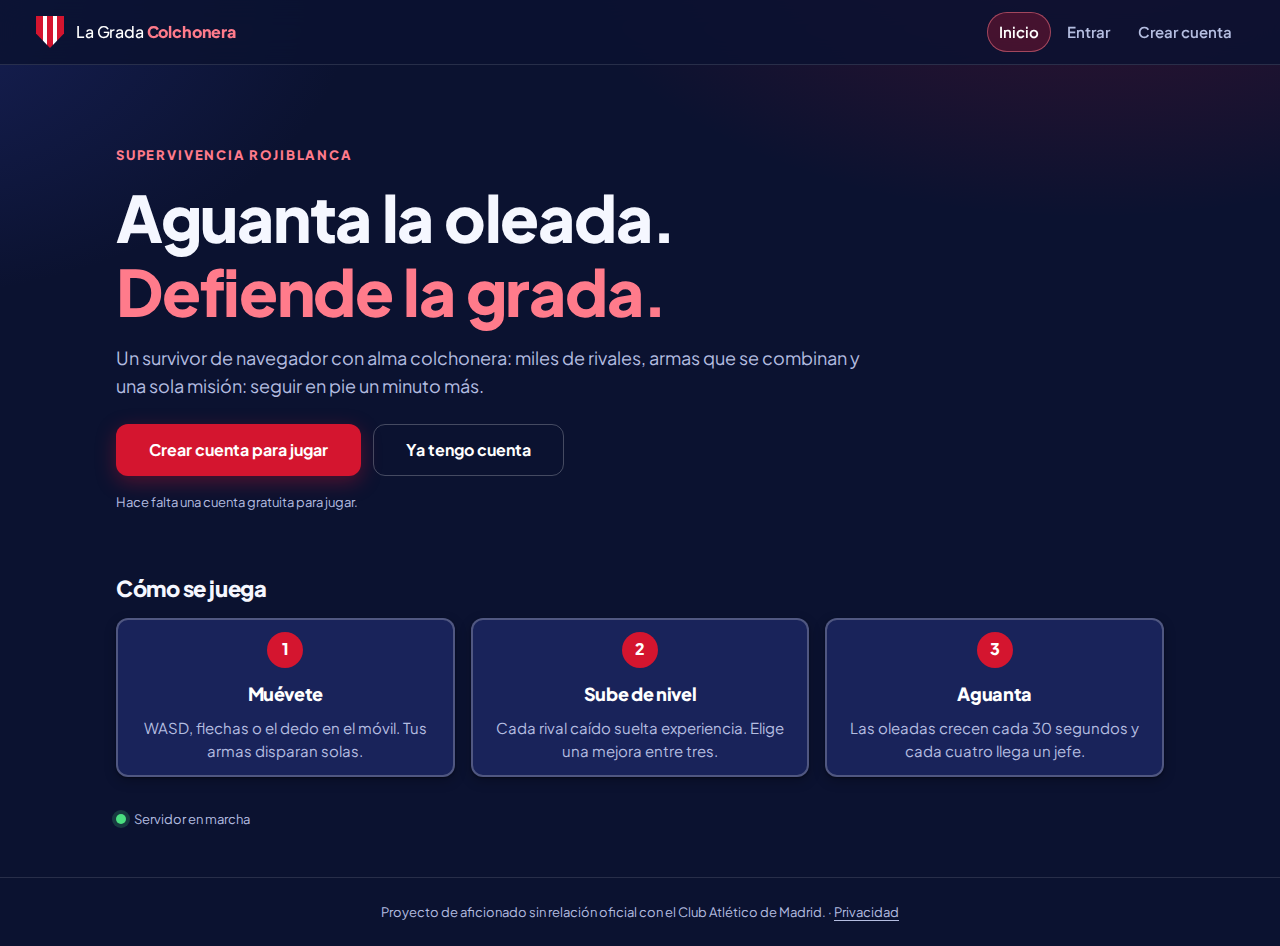
\includegraphics[width=0.9\textwidth]{figs/capturas/app/01-inicio.png}
\caption{Página de inicio sin sesión: botones para crear cuenta o entrar, cómo se juega y estado del servidor (P7).}
\label{fig:app-inicio}
\end{figure}

\begin{figure}[htbp]
\centering
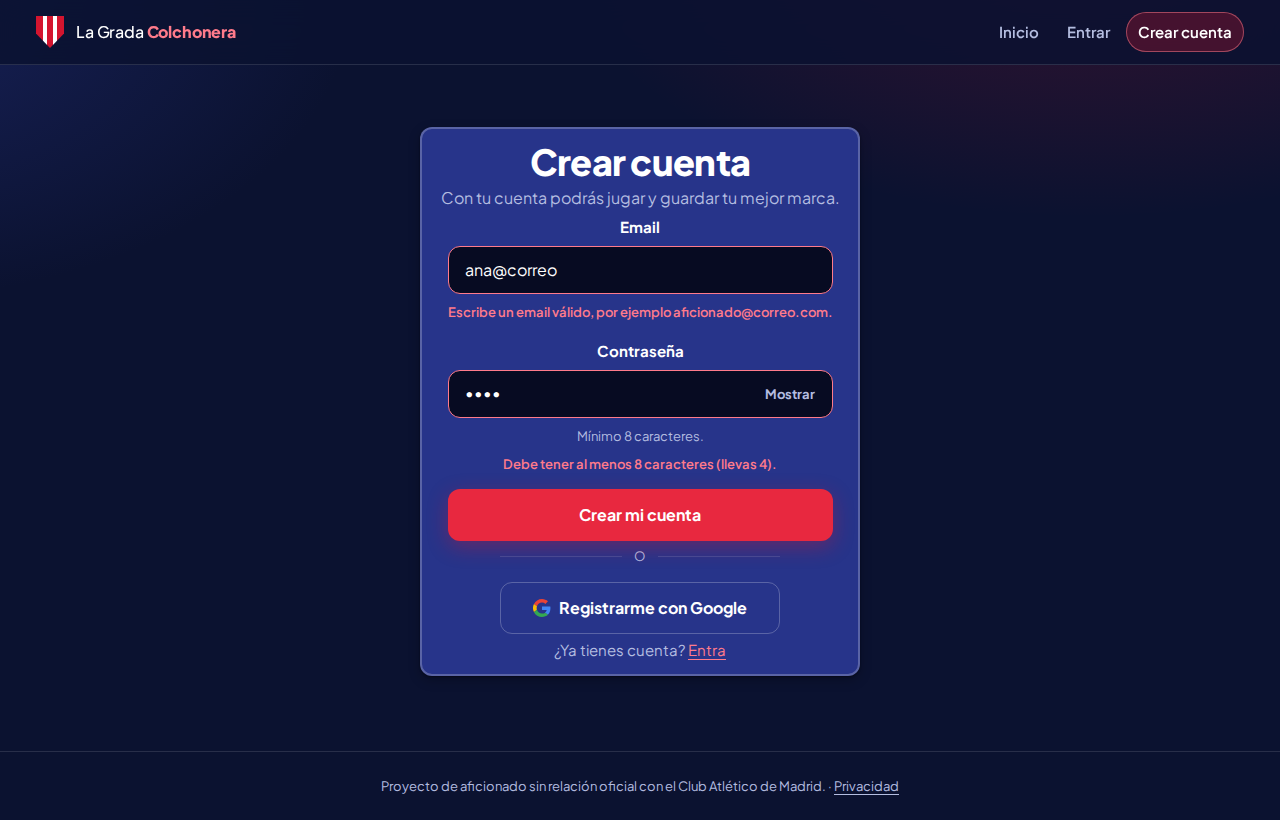
\includegraphics[width=0.9\textwidth]{figs/capturas/app/02-registro-validacion.png}
\caption{Registro con email y contraseña no válidos: campos en rojo y errores explicados (RF-01, RF-12).}
\label{fig:app-registro-val}
\end{figure}

\begin{figure}[htbp]
\centering
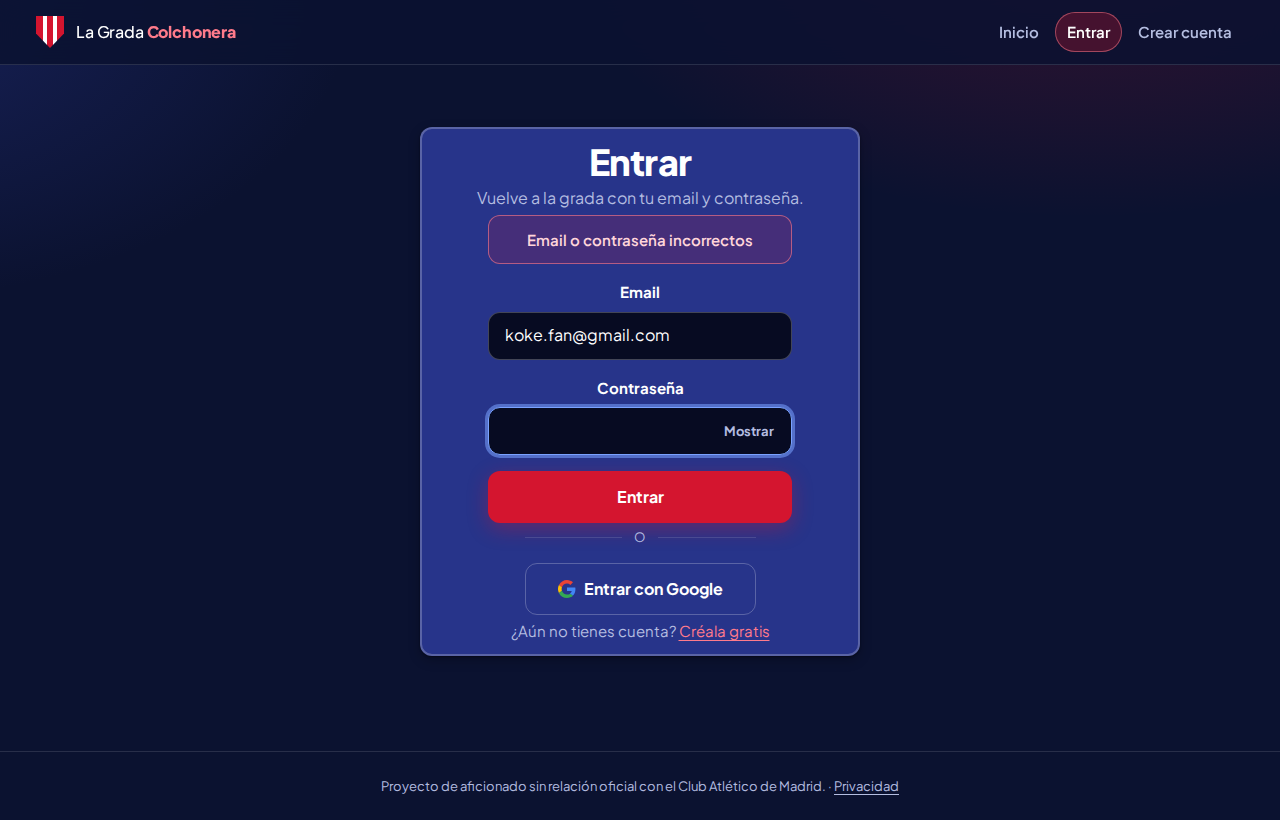
\includegraphics[width=0.9\textwidth]{figs/capturas/app/03-entrar-error.png}
\caption{Entrar con contraseña incorrecta: «Email o contraseña incorrectos» (RF-02, RF-12).}
\label{fig:app-login-err}
\end{figure}

\begin{figure}[htbp]
\centering
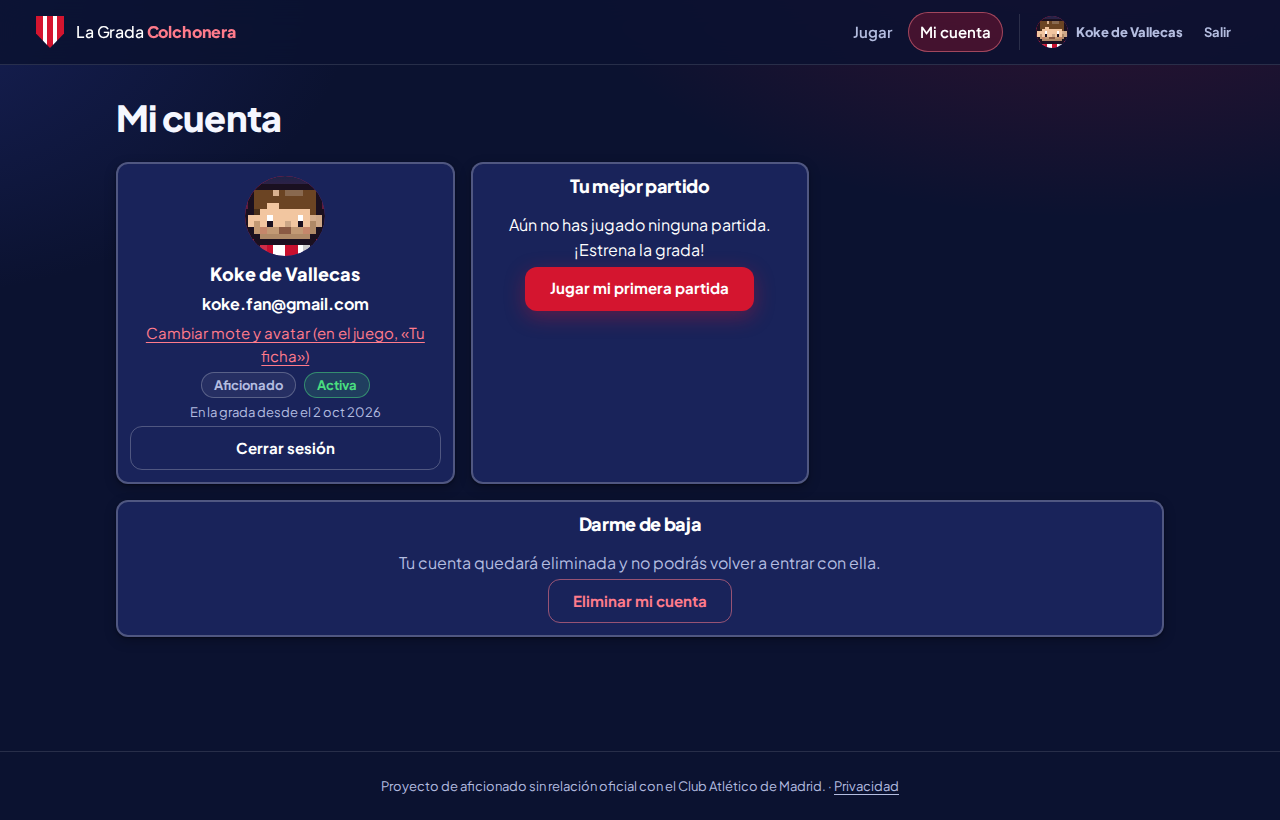
\includegraphics[width=0.9\textwidth]{figs/capturas/app/04-perfil.png}
\caption{Mi cuenta: mote, avatar, email, rol Aficionado, estado Activa, fecha de alta, cerrar sesión y darse de baja (RF-03, RF-08, RF-09).}
\label{fig:app-perfil}
\end{figure}

La Figura~\ref{fig:app-baja-conf} muestra el diálogo de confirmación antes de la baja. La Figura~\ref{fig:app-sin-permiso} ilustra la redirección de un usuario normal que intenta acceder a administración.

\begin{figure}[htbp]
\centering
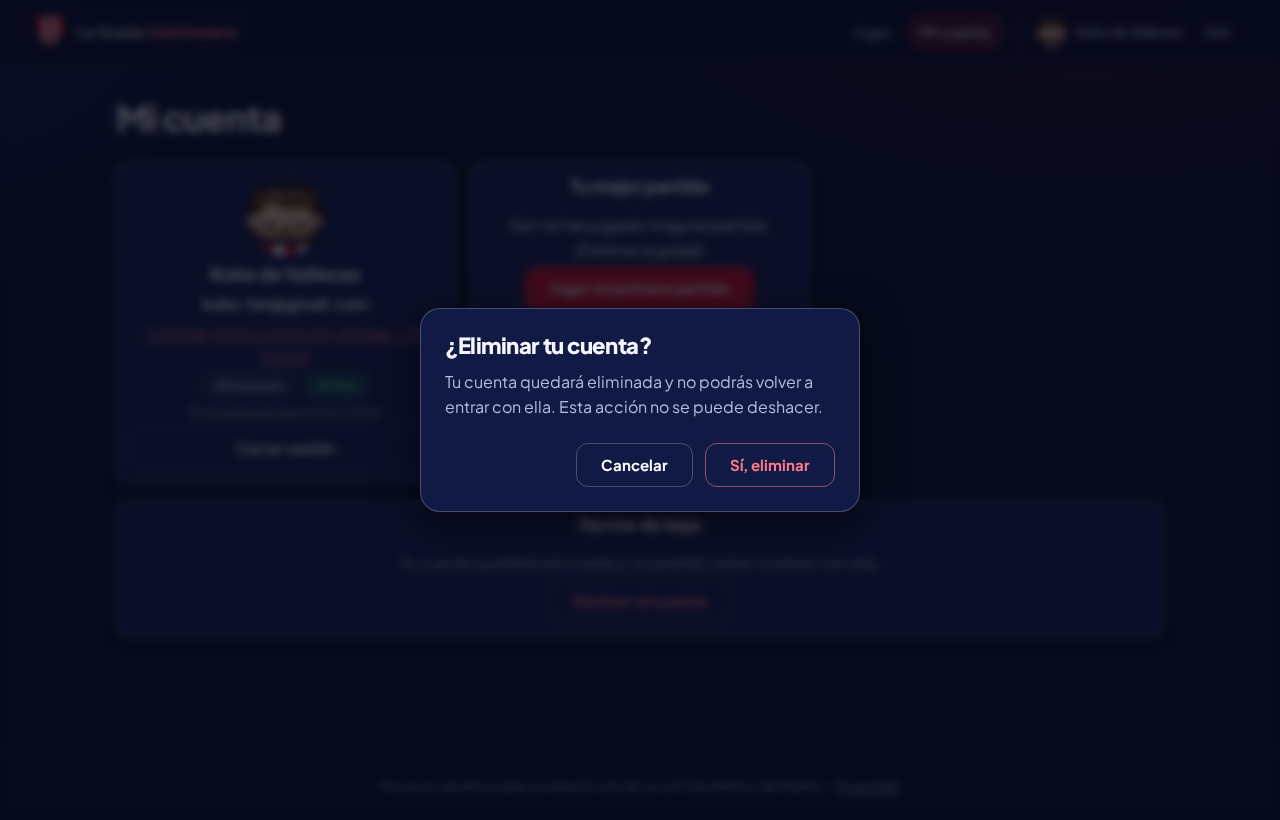
\includegraphics[width=0.9\textwidth]{figs/capturas/app/05-confirmar-baja.png}
\caption{Diálogo «¿Eliminar tu cuenta?» antes de darse de baja (RF-08, RF-12).}
\label{fig:app-baja-conf}
\end{figure}

\begin{figure}[htbp]
\centering
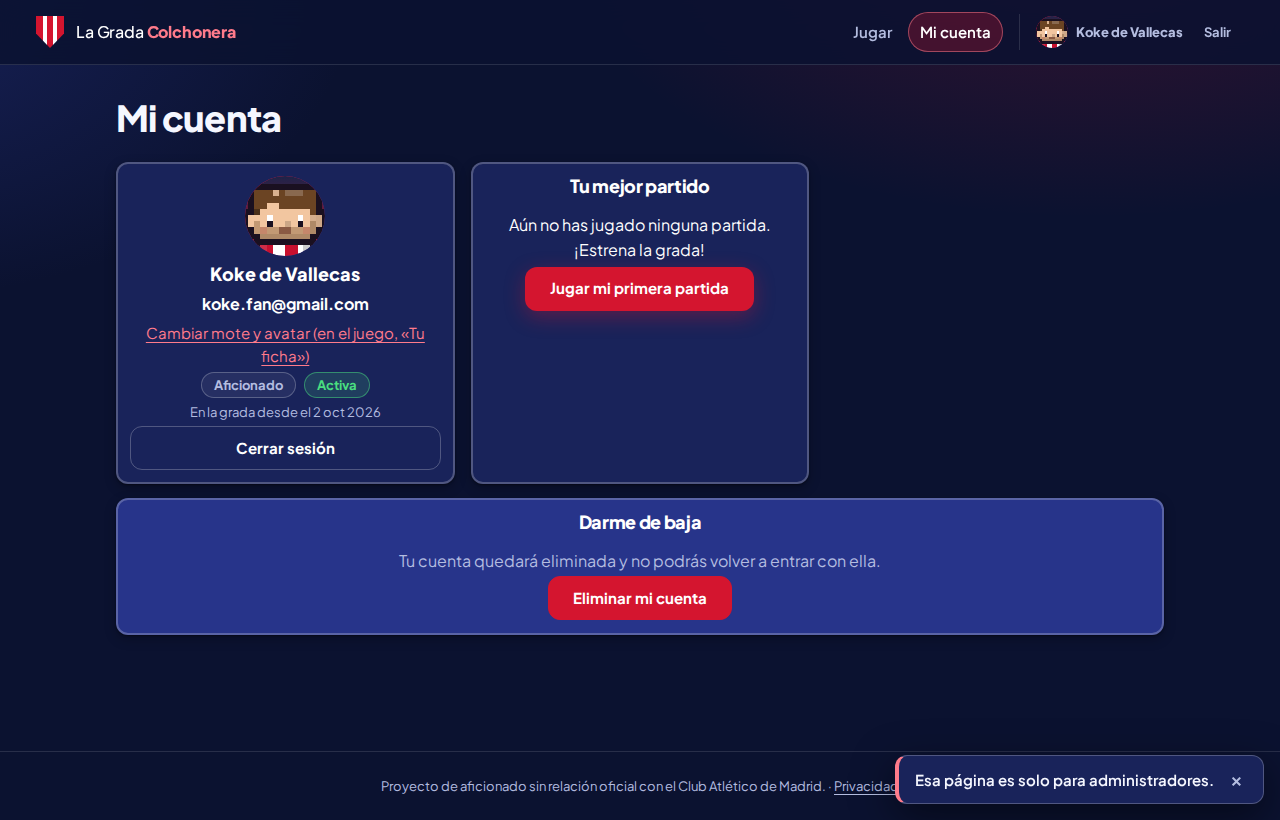
\includegraphics[width=0.9\textwidth]{figs/capturas/app/06-usuario-sin-permiso.png}
\caption{Usuario normal intenta abrir \texttt{\#/admin} y vuelve a Mi cuenta con aviso «Esa página es solo para administradores» (RF-04, RF-07).}
\label{fig:app-sin-permiso}
\end{figure}

\subsection{Panel de administración}

Las Figuras~\ref{fig:app-admin} a \ref{fig:app-admin-movil} muestran el panel de administración: listado con buscador, estados vacíos, confirmación de eliminación y vista responsive en móvil.

\begin{figure}[htbp]
\centering
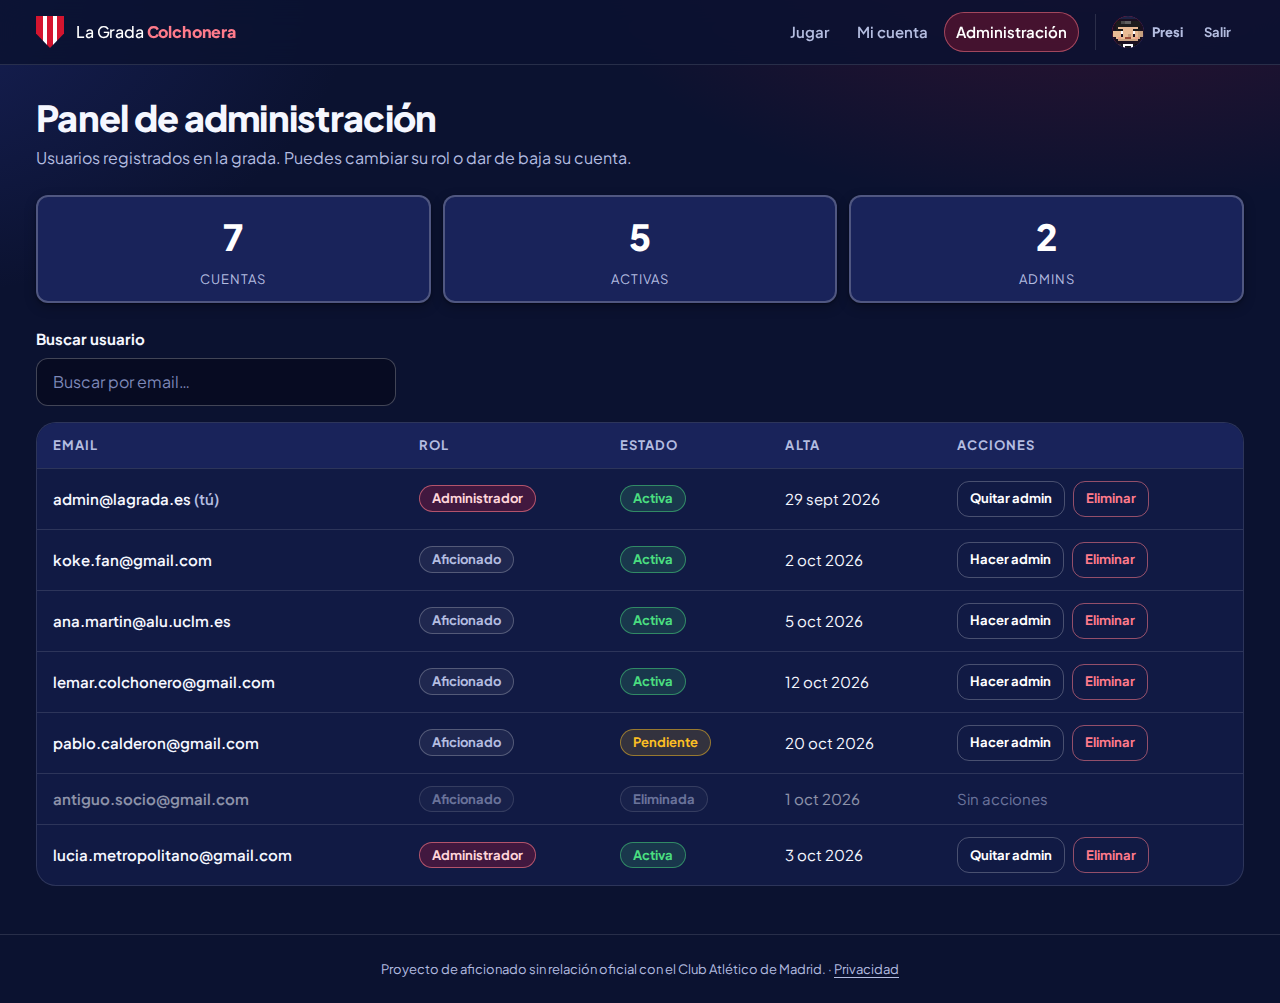
\includegraphics[width=0.9\textwidth]{figs/capturas/app/07-panel-admin.png}
\caption{Panel de administración: contadores, buscador y tabla con email, rol, estado, alta y acciones (RF-07).}
\label{fig:app-admin}
\end{figure}

\begin{figure}[htbp]
\centering
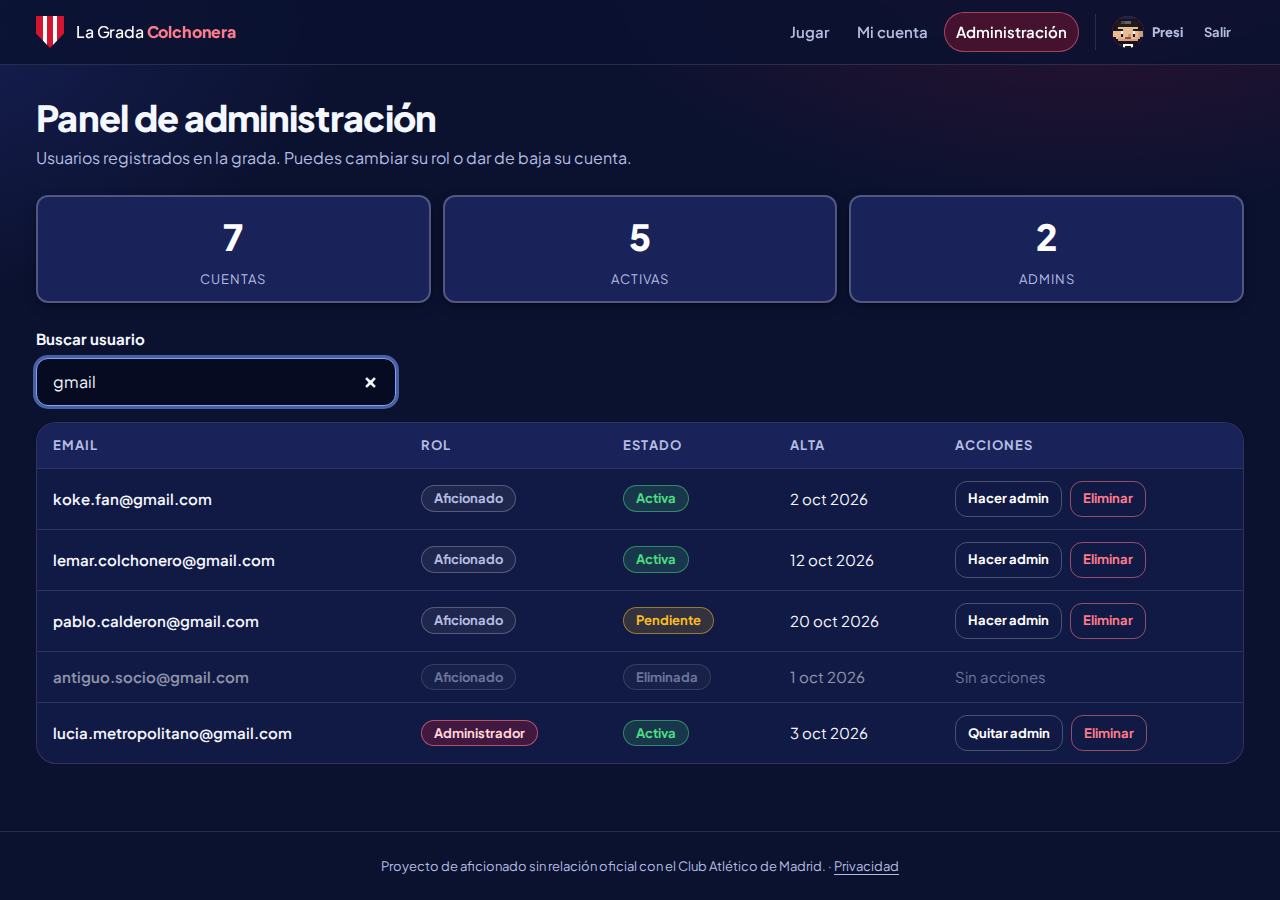
\includegraphics[width=0.9\textwidth]{figs/capturas/app/08-admin-busqueda.png}
\caption{Panel filtrado por email (RF-07).}
\label{fig:app-admin-busqueda}
\end{figure}

\begin{figure}[htbp]
\centering
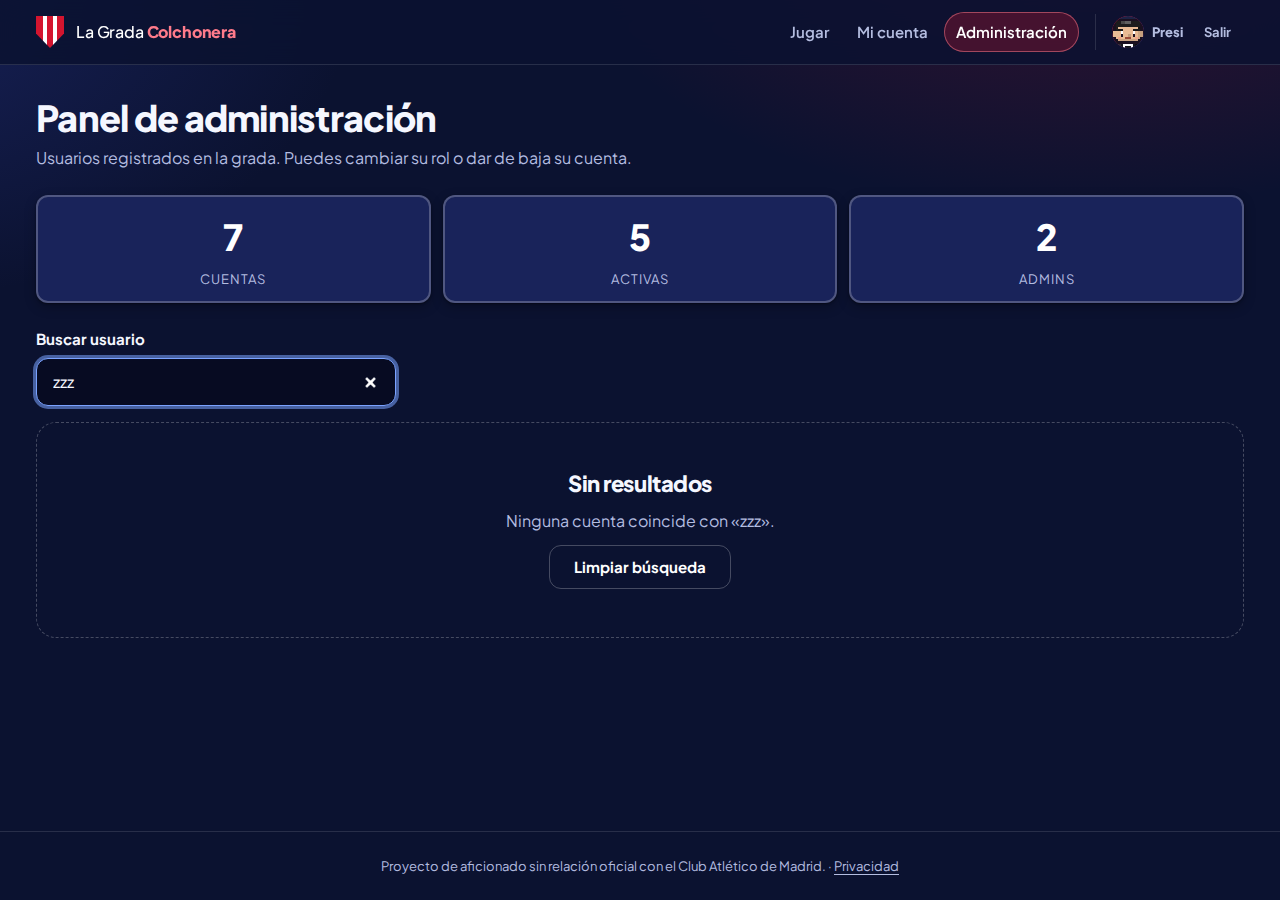
\includegraphics[width=0.9\textwidth]{figs/capturas/app/09-admin-sin-resultados.png}
\caption{Estado vacío de la búsqueda con botón «Limpiar búsqueda» (RF-12).}
\label{fig:app-admin-vacio}
\end{figure}

\begin{figure}[htbp]
\centering
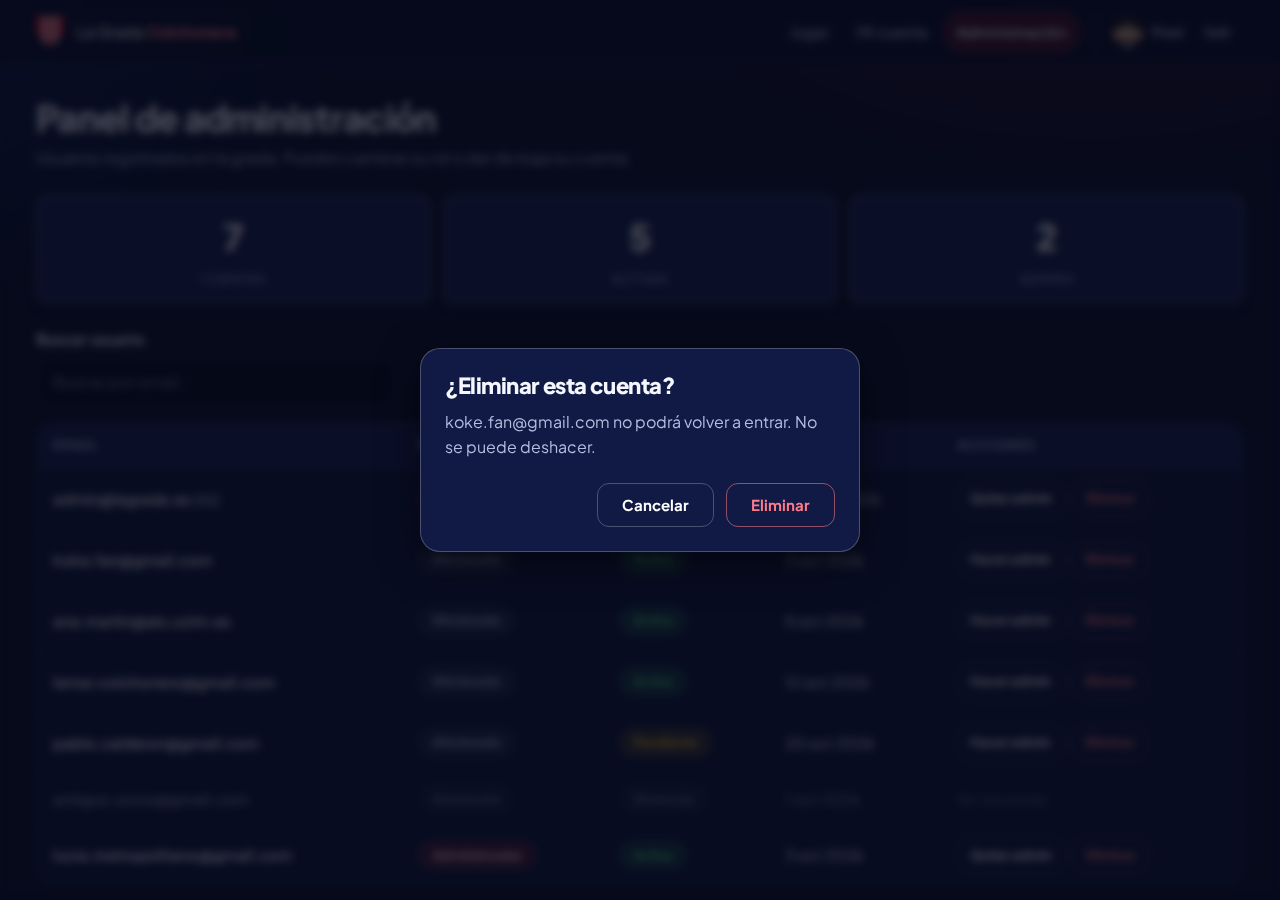
\includegraphics[width=0.9\textwidth]{figs/capturas/app/10-admin-confirmar-eliminar.png}
\caption{Diálogo de confirmación antes de eliminar otra cuenta desde el panel (RF-08).}
\label{fig:app-admin-del-conf}
\end{figure}

\begin{figure}[htbp]
\centering
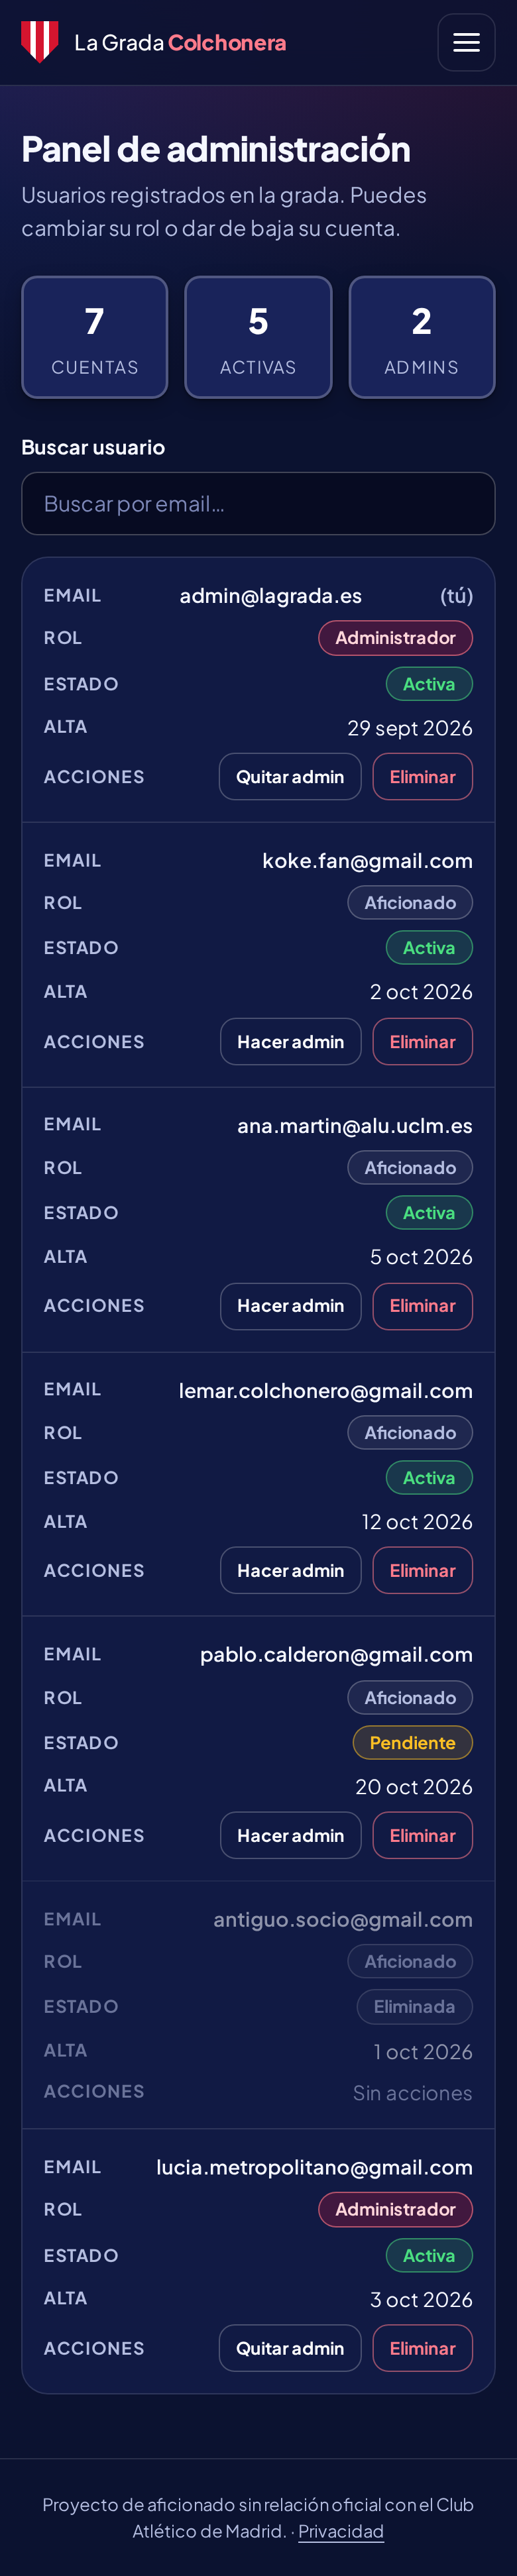
\includegraphics[width=0.35\textwidth]{figs/capturas/app/11-panel-admin-movil.png}
\caption{Panel de administración en móvil: cada usuario es una tarjeta (RNF-08).}
\label{fig:app-admin-movil}
\end{figure}

\begin{figure}[htbp]
\centering
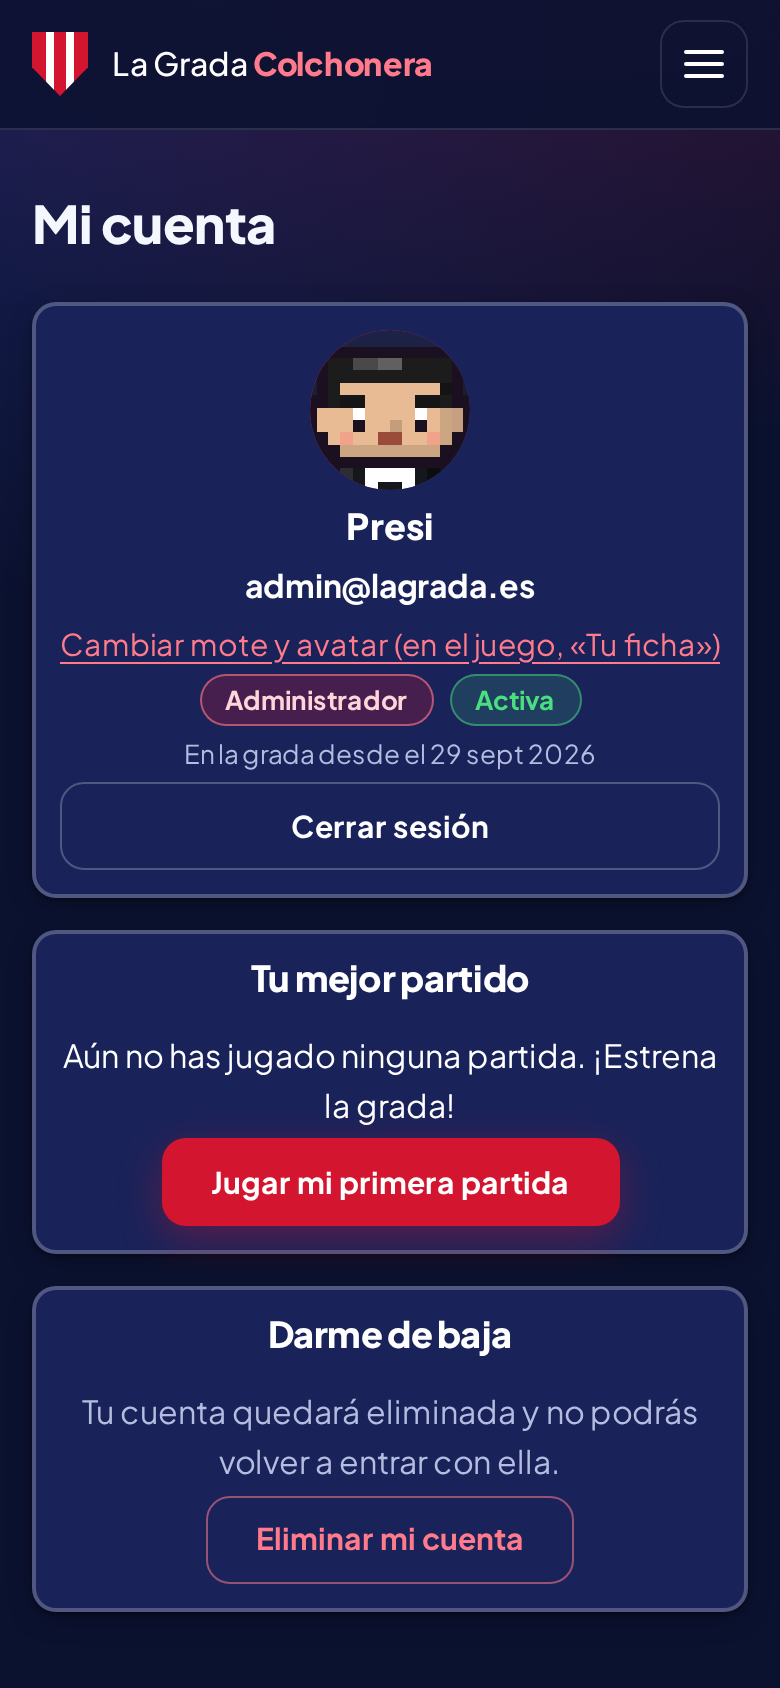
\includegraphics[width=0.35\textwidth]{figs/capturas/app/12-perfil-movil.png}
\caption{Mi cuenta en móvil con menú plegado (RNF-08).}
\label{fig:app-perfil-movil}
\end{figure}

\subsection{Hito 4: correo, Google y errores}

La Figura~\ref{fig:hito4-google} muestra el botón «Entrar con Google». La Figura~\ref{fig:hito4-correo-enviado} el aviso tras registro con correo de confirmación. Las Figuras~\ref{fig:hito4-pendiente-reenvio} y \ref{fig:hito4-reenvio} cubren el error de cuenta pendiente y el reenvío. Las Figuras~\ref{fig:hito4-enlace-invalido} y \ref{fig:hito4-confirmada} muestran enlace manipulado y confirmación exitosa. La Figura~\ref{fig:hito4-primer-acceso} el primer acceso tras confirmar. La Figura~\ref{fig:hito4-google-creada} la cuenta nueva por Google. La Figura~\ref{fig:hito4-error-reintento} el estado de error con botón Reintentar. La Figura~\ref{fig:hito4-admin-estados} el panel con todos los estados de cuenta. La Figura~\ref{fig:hito4-privacidad} la política de privacidad.

\begin{figure}[htbp]
\centering
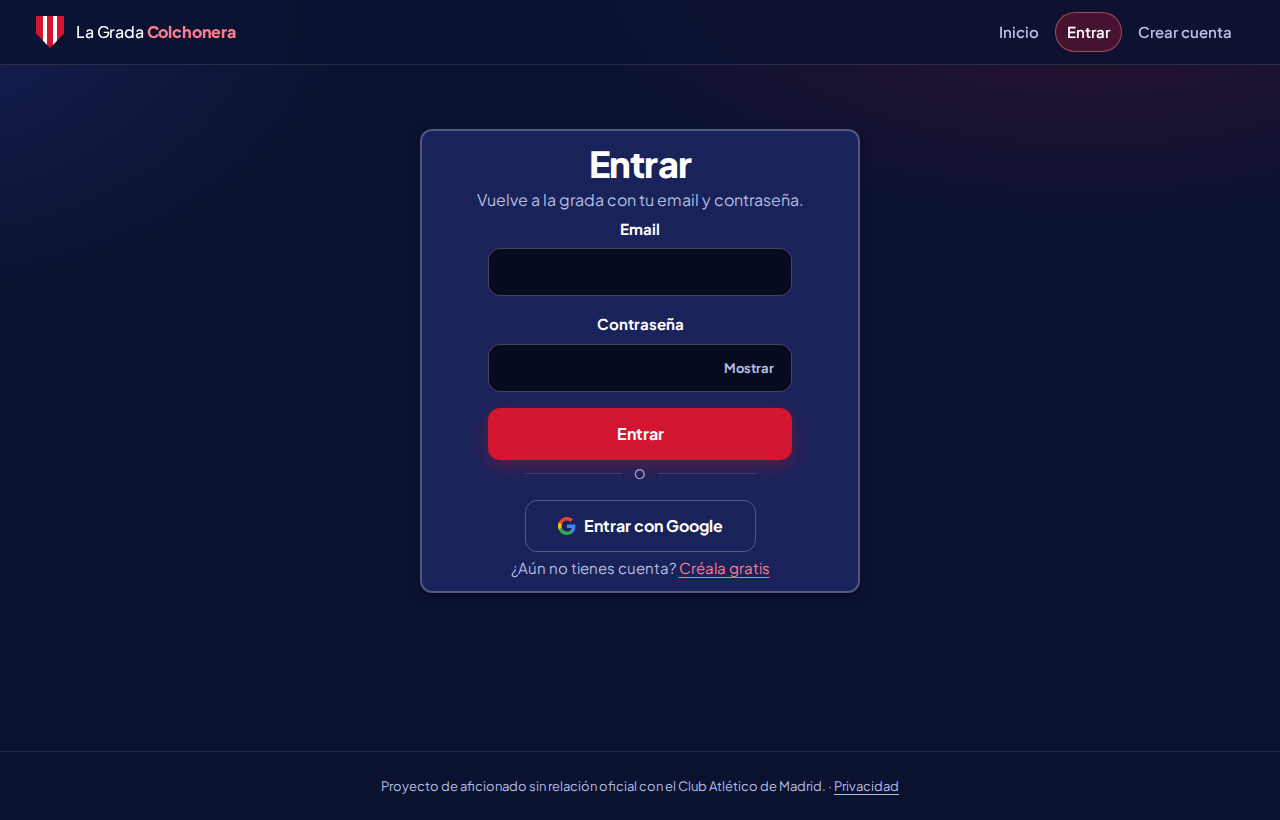
\includegraphics[width=0.9\textwidth]{figs/capturas/hito4/01-entrar-google.png}
\caption{Pantalla de entrar con el botón «Entrar con Google» (RF-11).}
\label{fig:hito4-google}
\end{figure}

\begin{figure}[htbp]
\centering
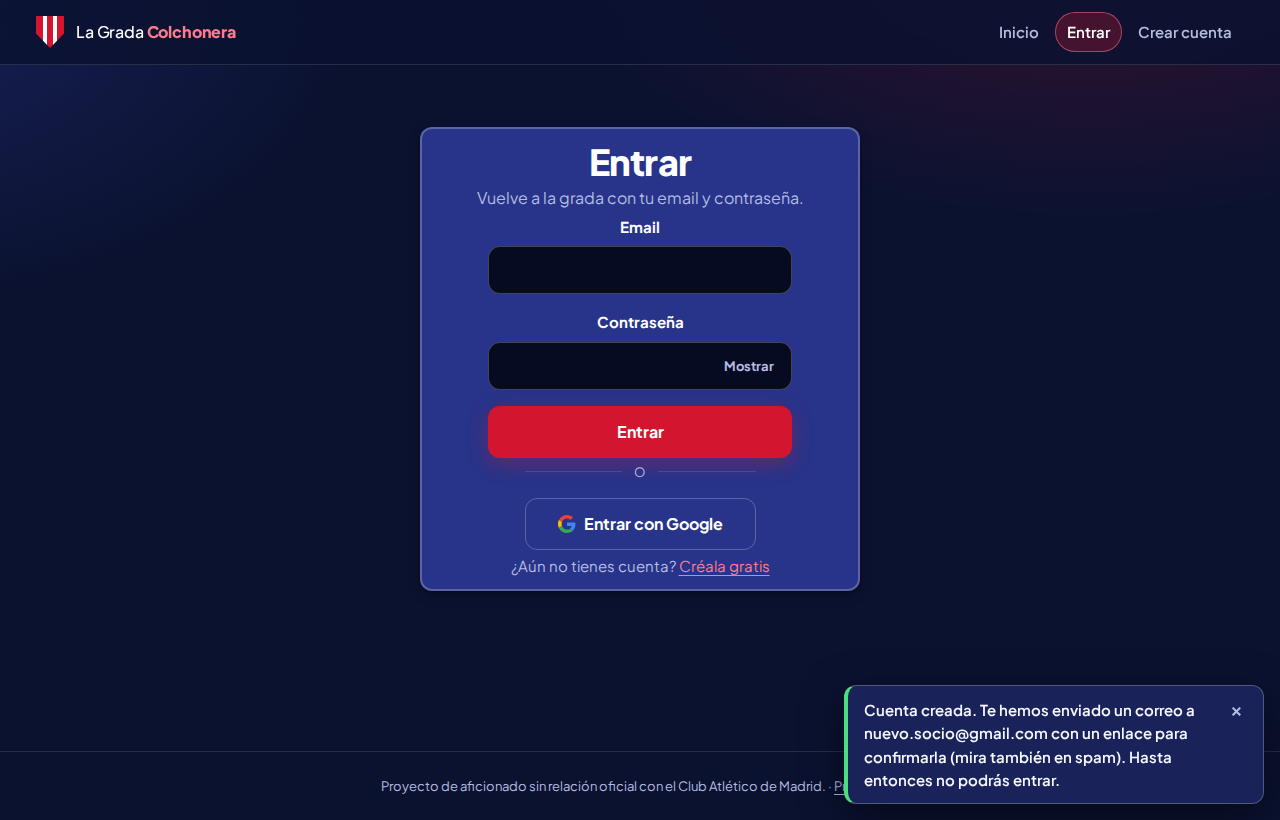
\includegraphics[width=0.9\textwidth]{figs/capturas/hito4/02-registro-correo-enviado.png}
\caption{Registro: aviso de cuenta creada y correo de confirmación enviado (RF-10).}
\label{fig:hito4-correo-enviado}
\end{figure}

\begin{figure}[htbp]
\centering
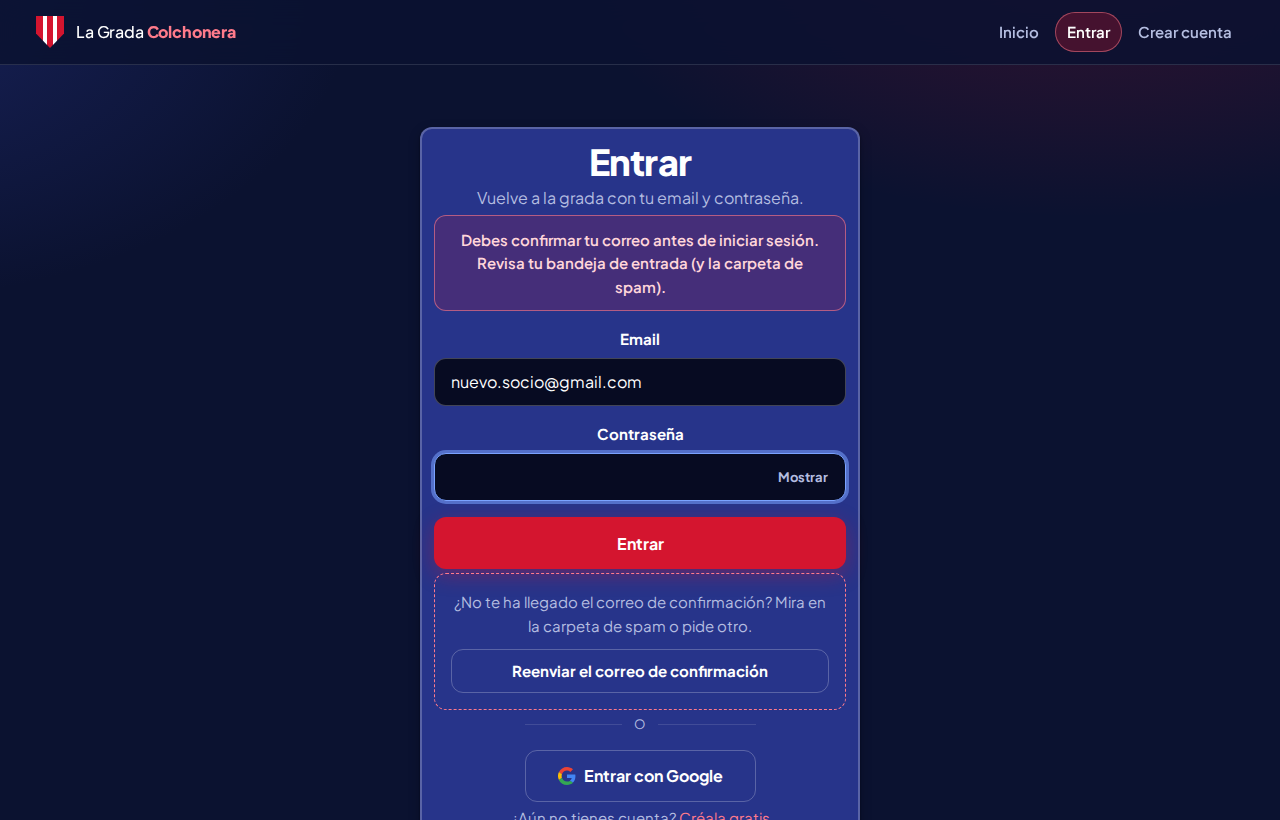
\includegraphics[width=0.9\textwidth]{figs/capturas/hito4/03-cuenta-pendiente-reenvio.png}
\caption{Login de cuenta pendiente: error y botón «Reenviar el correo de confirmación» (RF-10, RF-12).}
\label{fig:hito4-pendiente-reenvio}
\end{figure}

\begin{figure}[htbp]
\centering
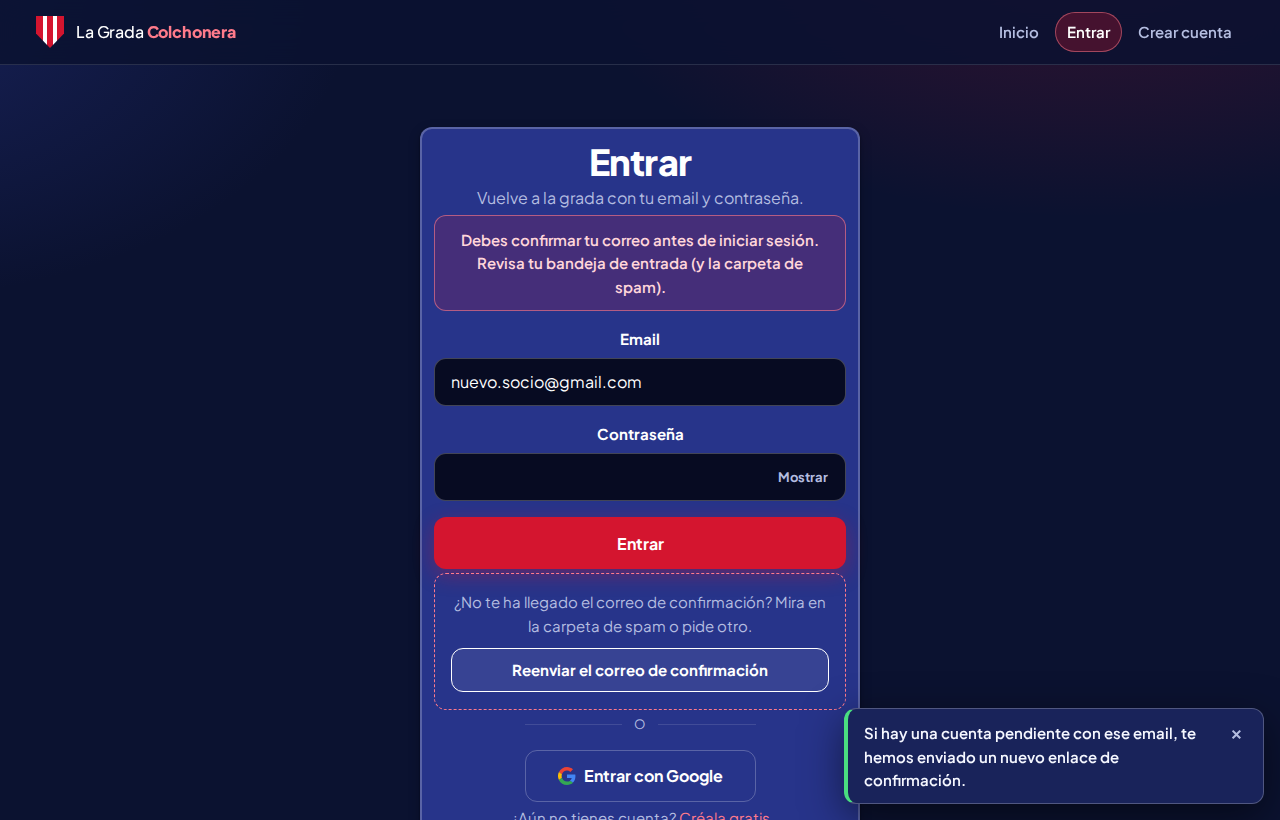
\includegraphics[width=0.9\textwidth]{figs/capturas/hito4/04-reenvio-hecho.png}
\caption{Aviso de reenvío (no revela si la cuenta existe) (RF-10).}
\label{fig:hito4-reenvio}
\end{figure}

\begin{figure}[htbp]
\centering
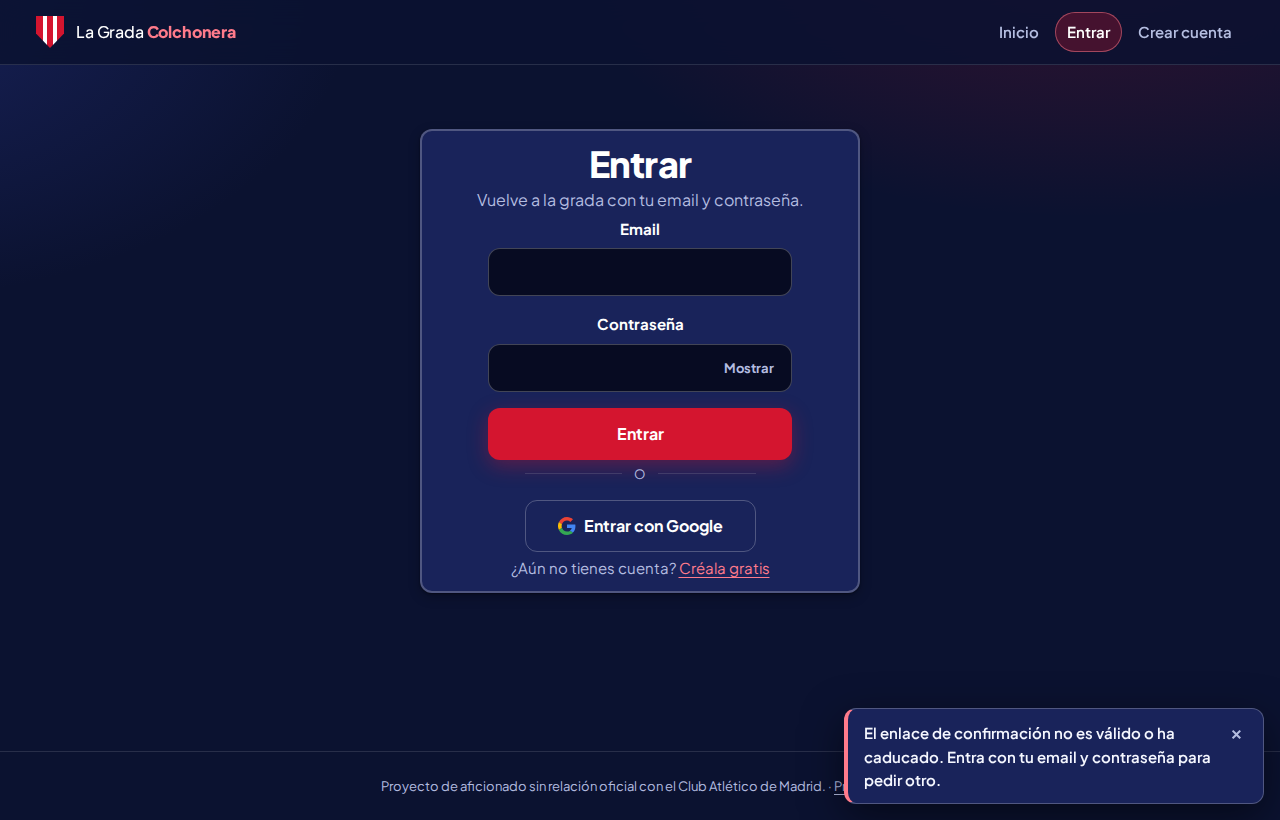
\includegraphics[width=0.9\textwidth]{figs/capturas/hito4/05-enlace-invalido.png}
\caption{Enlace manipulado o caducado: aviso rojo, la cuenta sigue pendiente (RF-10, RF-12).}
\label{fig:hito4-enlace-invalido}
\end{figure}

\begin{figure}[htbp]
\centering
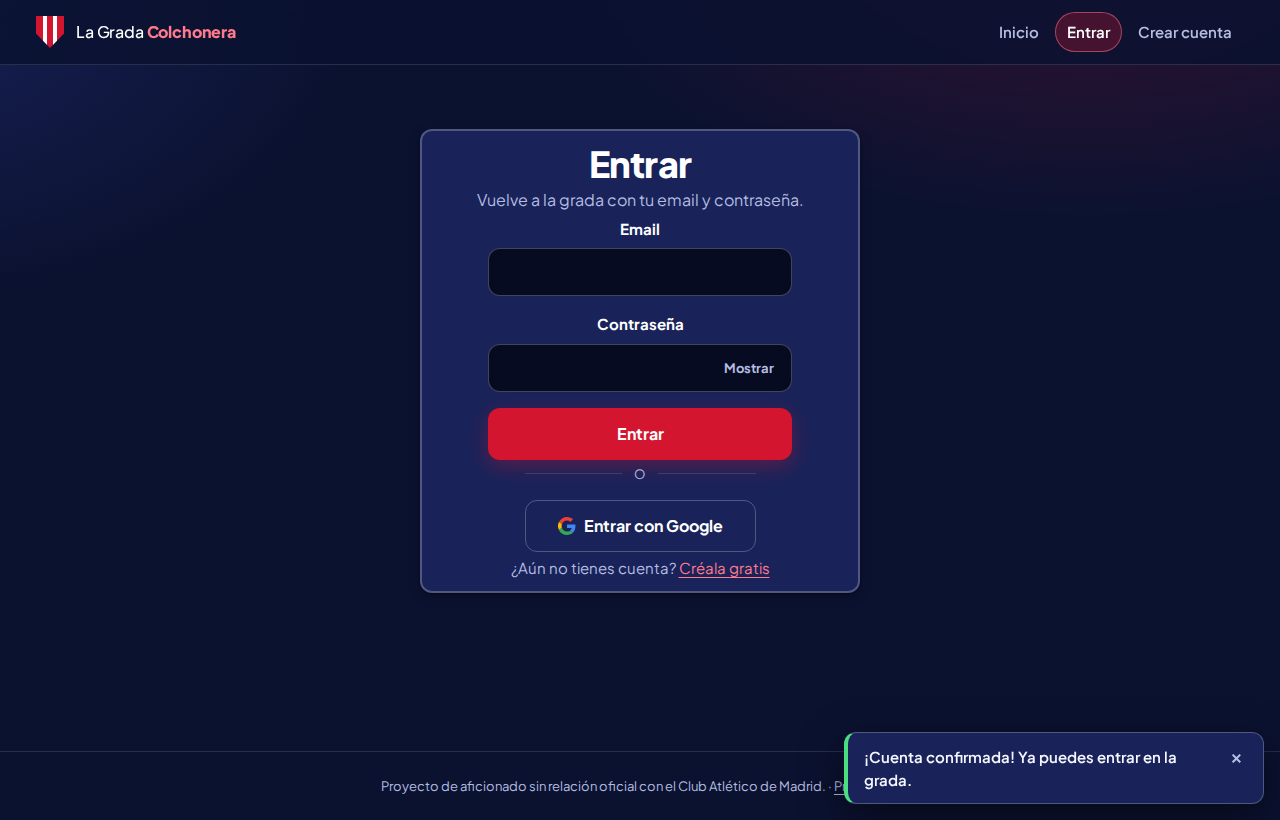
\includegraphics[width=0.9\textwidth]{figs/capturas/hito4/06-cuenta-confirmada.png}
\caption{Enlace correcto: aviso verde de cuenta confirmada (RF-10).}
\label{fig:hito4-confirmada}
\end{figure}

\begin{figure}[htbp]
\centering
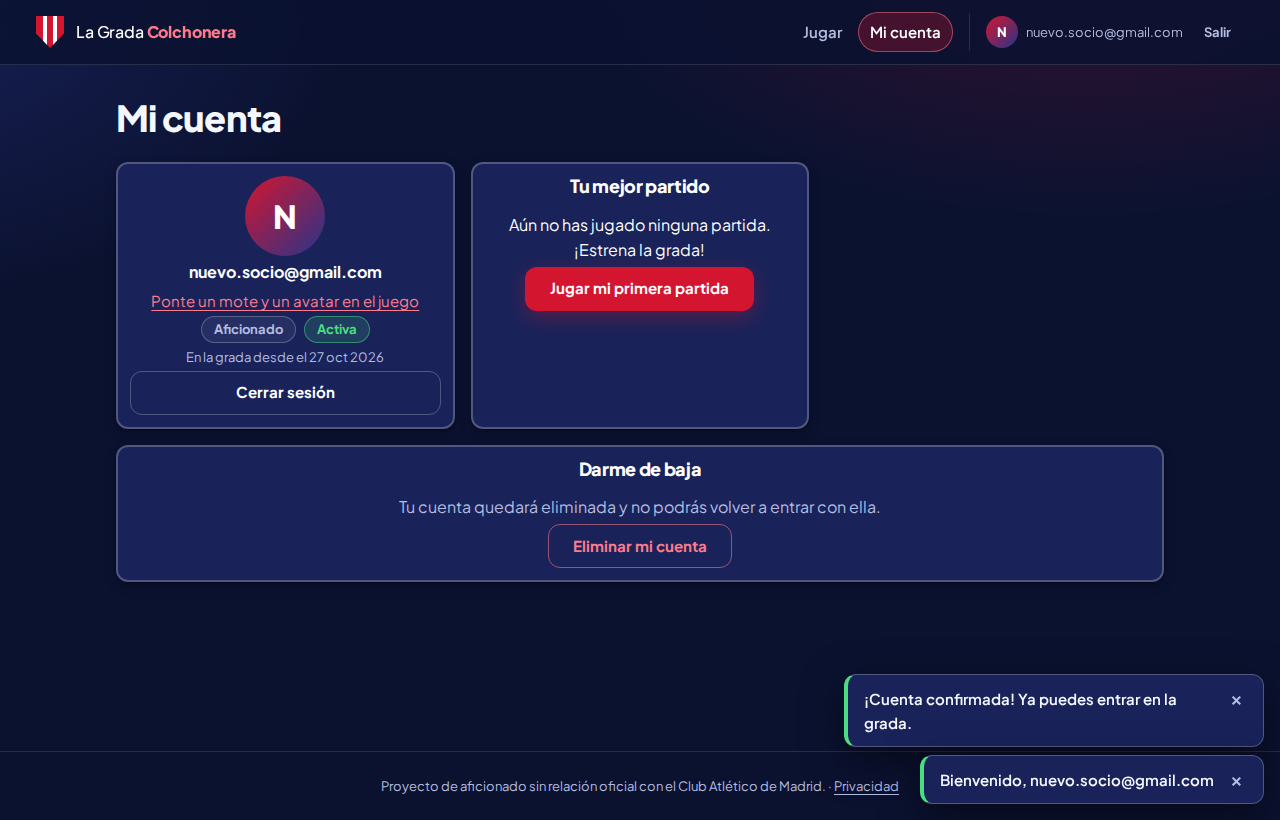
\includegraphics[width=0.9\textwidth]{figs/capturas/hito4/07-primer-acceso.png}
\caption{Primer acceso tras confirmar: Mi cuenta con aviso de bienvenida (RF-10).}
\label{fig:hito4-primer-acceso}
\end{figure}

\begin{figure}[htbp]
\centering
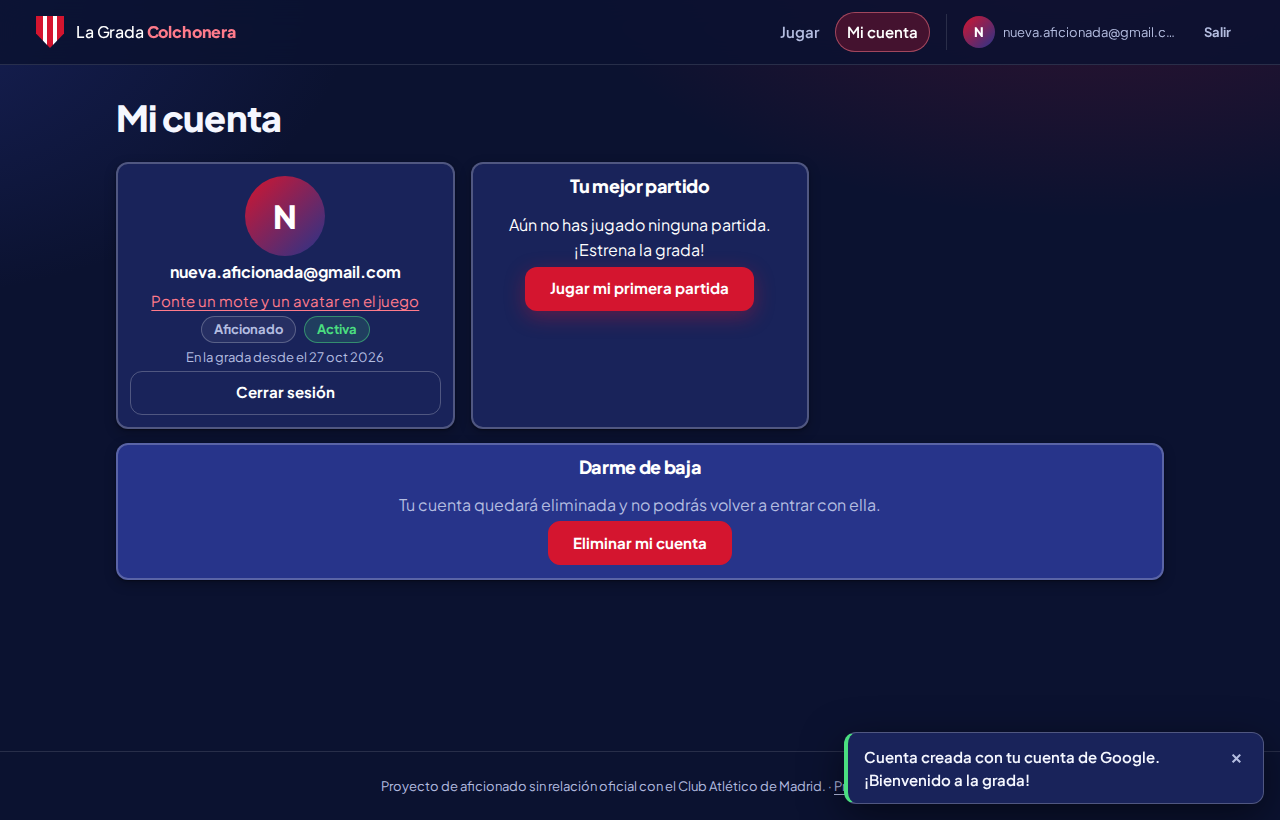
\includegraphics[width=0.9\textwidth]{figs/capturas/hito4/08-google-cuenta-creada.png}
\caption{Cuenta nueva con Google: Mi cuenta con aviso «Cuenta creada con tu cuenta de Google» (RF-11).}
\label{fig:hito4-google-creada}
\end{figure}

\begin{figure}[htbp]
\centering
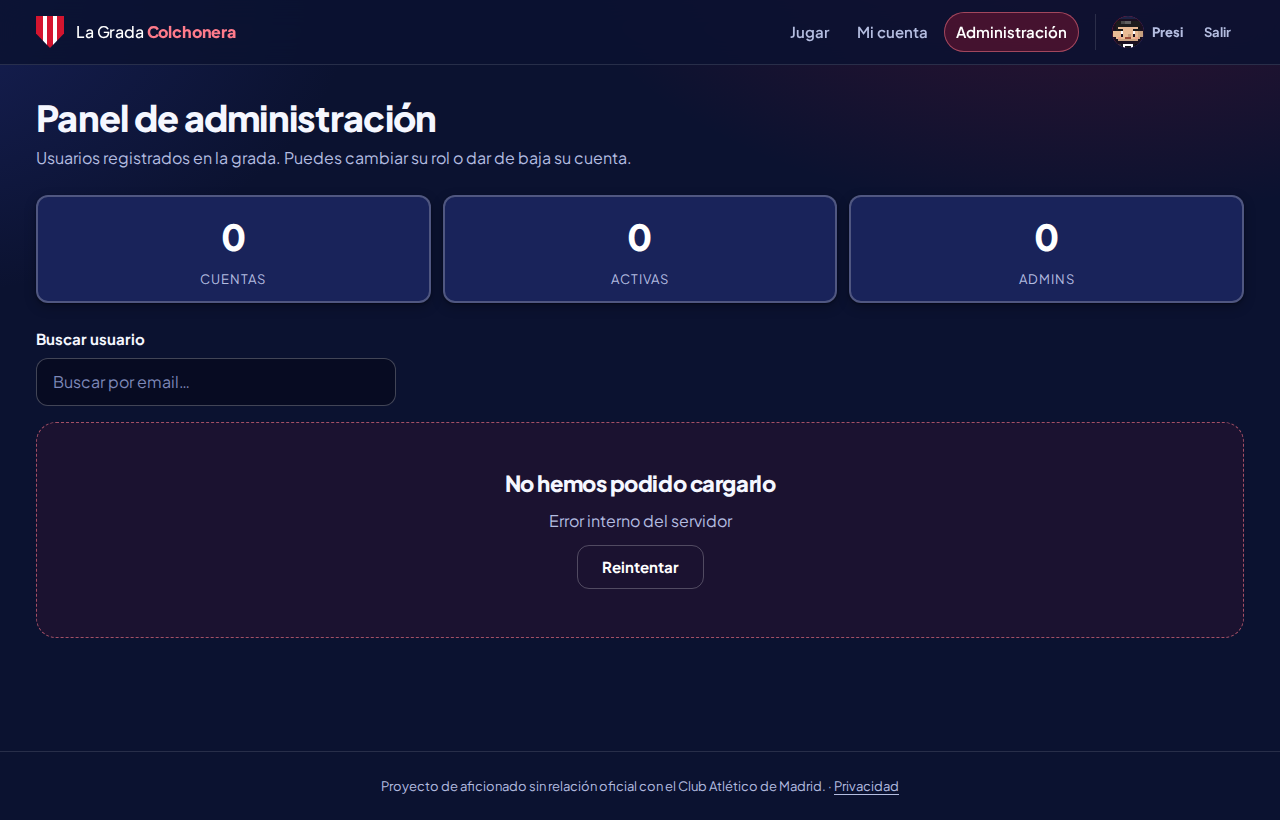
\includegraphics[width=0.9\textwidth]{figs/capturas/hito4/09-error-con-reintento.png}
\caption{Fallo del servidor al cargar el panel: «No hemos podido cargarlo» con botón Reintentar (RF-12).}
\label{fig:hito4-error-reintento}
\end{figure}

\begin{figure}[htbp]
\centering
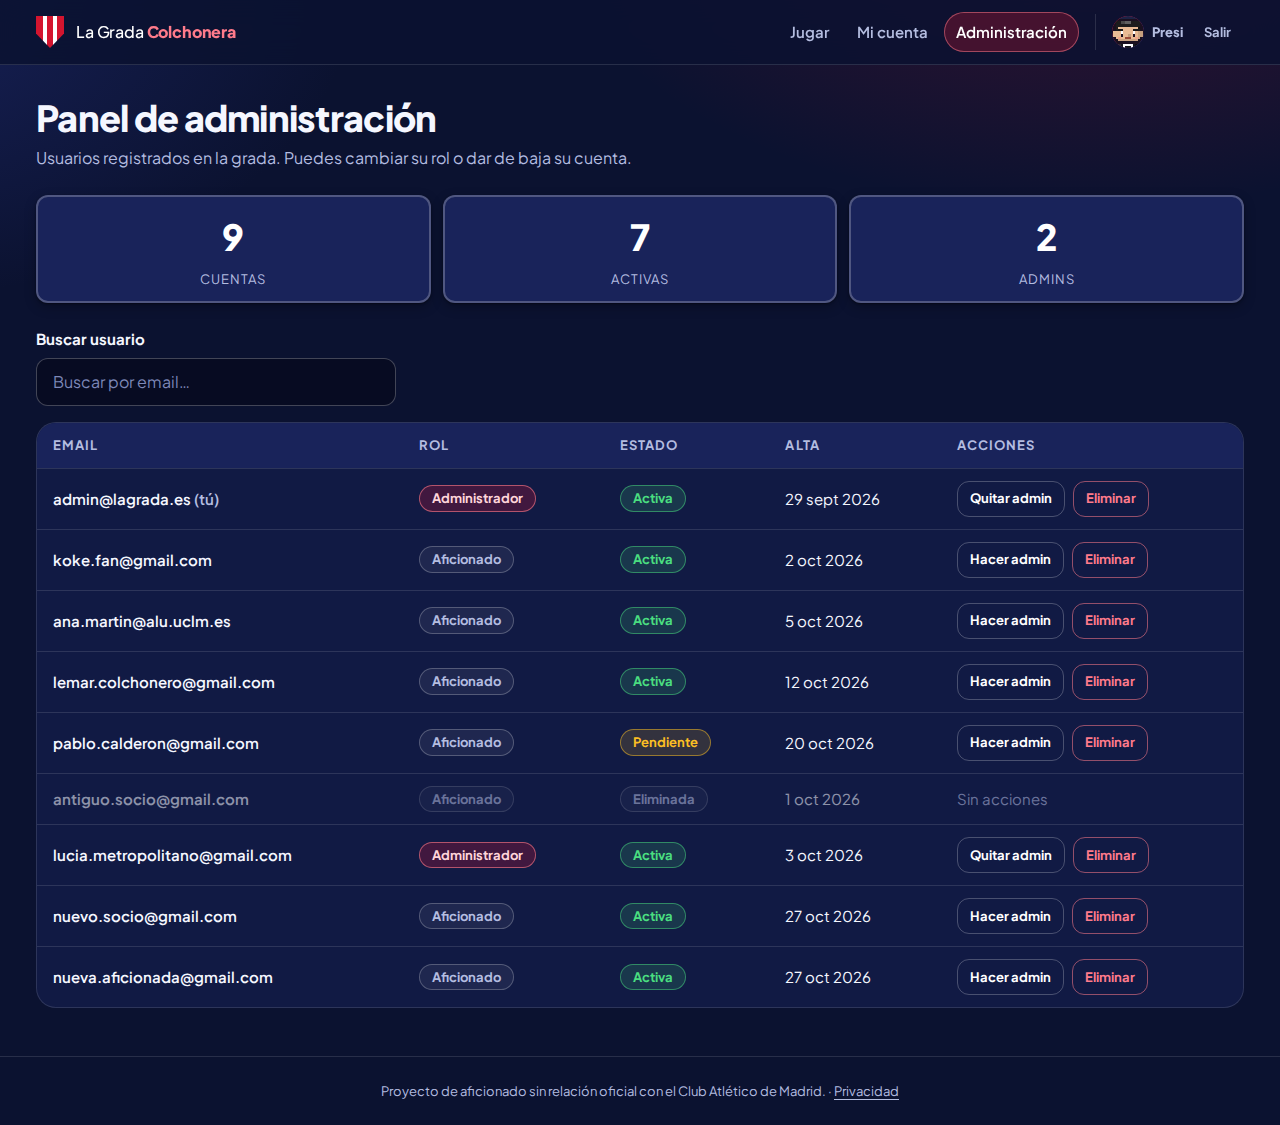
\includegraphics[width=0.9\textwidth]{figs/capturas/hito4/10-panel-admin-estados.png}
\caption{Panel con cuentas activas, pendientes, eliminadas, locales y de Google (RF-07, RF-11, RF-10).}
\label{fig:hito4-admin-estados}
\end{figure}

\begin{figure}[htbp]
\centering
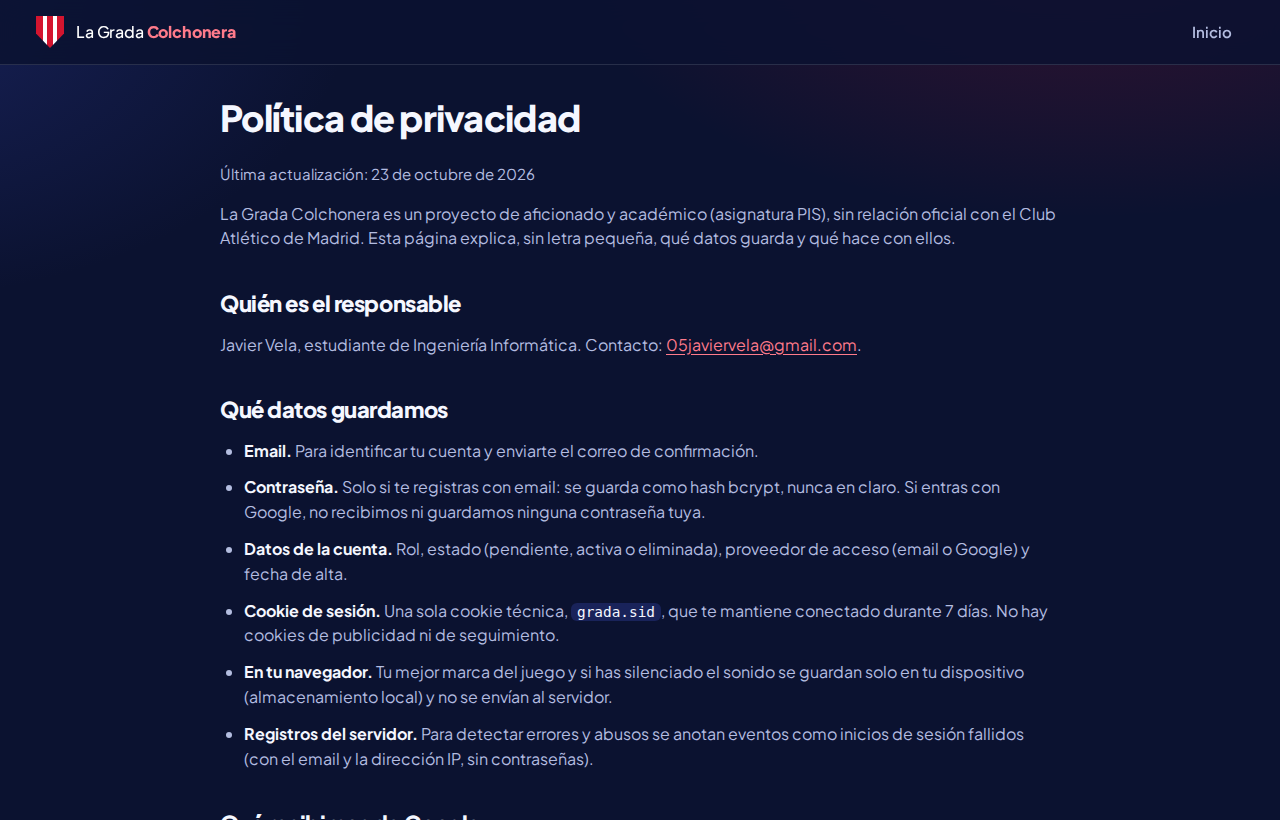
\includegraphics[width=0.9\textwidth]{figs/capturas/hito4/11-privacidad.png}
\caption{Política de privacidad (RNF-11).}
\label{fig:hito4-privacidad}
\end{figure}

La ruta inexistente muestra «Fuera de juego» (Figura~\ref{fig:app-404}).

\begin{figure}[htbp]
\centering
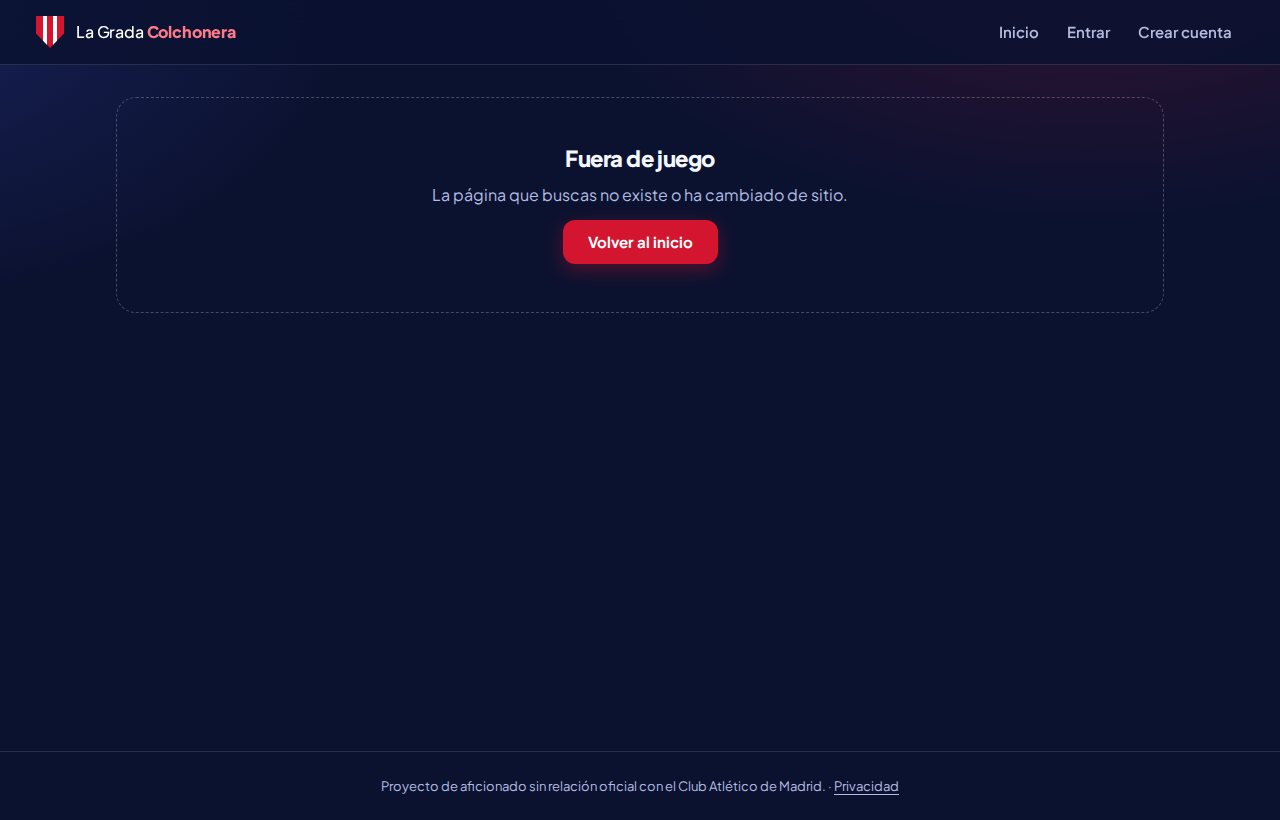
\includegraphics[width=0.9\textwidth]{figs/capturas/app/13-pagina-no-encontrada.png}
\caption{Ruta inexistente: «Fuera de juego» (RF-12).}
\label{fig:app-404}
\end{figure}

Todas las capturas proceden de \texttt{figs/capturas/app/} y \texttt{figs/capturas/hito4/} (documentacion-tecnica.md §16). El subsistema SaaS queda así completamente documentado; el juego se detalla en el Capítulo~\ref{cap:juego}.

\chapter{Evaluación}
\label{cap:evaluacion}

\section{Diseño de la evaluación}

La evaluación de la calidad y del cumplimiento de la especificación se diseñó como un proceso multicapa continuo y reproducible. El marco de verificación descansa en cuatro pilares metodológicos:
\begin{enumerate}
    \item \textbf{Pruebas unitarias e integración en local:} Uso del ejecutor nativo \texttt{node:test} con el simulador de base de datos en memoria \texttt{pg-mem}, lo que permite ejecutar la suite completa en el entorno de desarrollo mediante el comando unificado \texttt{npm test}.
    \item \textbf{Integración continua en GitHub Actions:} Ejecución del flujo de trabajo automatizado en cada pull request y push hacia la rama \texttt{main}. Dicho flujo despliega un servicio PostgreSQL 17 real para ejecutar las pruebas contra la base de datos auténtica y valida la construcción de la imagen de producción en Docker mediante un contenedor \texttt{node:22-alpine}.
    \item \textbf{Comprobación del despliegue en Google Cloud Run:} El flujo de despliegue valida la salud del servicio desplegado mediante un smoke test que realiza hasta 20 intentos de consulta contra el endpoint \texttt{/api/health}.
    \item \textbf{Revisión frase a frase contra la especificación:} Auditoría manual exhaustiva documentada en \texttt{docs/revision-entrega.md}, contrastando cada apartado del enunciado con su evidencia concreta en código y pruebas.
\end{enumerate}

\section{Resultados}

La ejecución de las pruebas y la infraestructura arrojaron los resultados cuantitativos reflejados a continuación:
\begin{itemize}
    \item \textbf{Batería de pruebas automatizadas:} Un total de 80 pruebas automatizadas (79 ejecutables en entorno local y 1 prueba de extremo a extremo que se ejecuta exclusivamente en el CI contra PostgreSQL 17). De ellas, 26 corresponden a pruebas unitarias de la lógica de negocio en \texttt{userService}, evaluando registros duplicados, cuentas pendientes, control del último administrador y permisos. Las restantes cubren autenticación (10), API de usuarios (11), contratos de repositorios (12), logger (6), configuración (5), migraciones (3), interfaz (3), arranque (2) y salud (1).
    \item \textbf{Métricas del código fuente:} El servidor en \texttt{src/} cuenta con 1.128 líneas de JavaScript; el frontend en \texttt{public/} suma 657 líneas; y las pruebas en \texttt{tests/} alcanzan 992 líneas repartidas en 13 ficheros. Se crearon 2 migraciones SQL (\texttt{users} y \texttt{session}).
    \item \textbf{Actividad en GitHub:} Se contabilizan 65 commits en \texttt{main} (33 de trabajo y 32 fusiones de pull request), 33 pull requests integrados y 33 ramas gestionadas. Se registraron 71 ejecuciones de GitHub Actions (el workflow CI completó 65 ejecuciones).
    \item \textbf{Despliegue productivo:} El último commit en \texttt{main} (\texttt{978098e}, PR \#32, 12/10/2026) se desplegó en Google Cloud Run en 58 s de forma automática.
    \item \textbf{Consumo de recursos en Neon (a fecha 12/10/2026):} 0,27 CU-h de cómputo (frente a 100 CU-h disponibles), 0,03 GB de almacenamiento (sobre un límite de 1 GB) y 0 GB de transferencia sobre un límite mensual de 5 GB \cite{neonlimits}.
\end{itemize}

\section{Discusión}

El diseño de la evaluación proporciona garantías sólidas respecto a la integridad funcional del software: ninguna rama pudo fusionarse sin que la batería completa de pruebas resultara exitosa en un entorno PostgreSQL idéntico al de producción. Asimismo, la revisión frase a frase permitió identificar discrepancias sutiles antes del cierre, como la restricción del endpoint de verificación de usuario activo, que originalmente estaba abierto al propio usuario y fue restringido al administrador en el PR \#30 para ceñirse fielmente al enunciado \cite{enunciado}.

No obstante, como observación crítica sobre el proceso, debe señalarse que los 33 commits de desarrollo quedaron registrados con fecha 12/10/2026. Si bien la estructura del historial es estrictamente incremental y respeta el flujo de ramas y pull requests individuales por tarea, la concentración temporal en una única jornada debe considerarse con transparencia ante la evaluación docente, al contrastarla con la expectativa pedagógica de un avance espaciado en el tiempo.

\chapter{Conclusiones y Trabajo Futuro}
\label{cap:conclusiones}

\section{Conclusiones}

El desarrollo del Sprint 1 ha permitido materializar con éxito los objetivos planteados al inicio de la memoria, combinando la construcción de una aplicación funcional con la adhesión estricta a un proceso riguroso de ingeniería del software:
\begin{itemize}
    \item \textbf{Objetivo principal:} Se diseñó, implementó y desplegó en producción la arquitectura base de un servicio SaaS con gestión integral de usuarios, automatizando por completo el flujo desde la codificación hasta la entrega en la nube.
    \item \textbf{Diseño arquitectural desacoplado:} Se estructuró el backend en capas bien diferenciadas (API, lógica y datos) servidas desde el mismo origen que el cliente web, garantizando la independencia y modularidad del sistema.
    \item \textbf{Gestión de identidades y sesiones:} Se implementó la autenticación local con derivación de contraseñas mediante \texttt{bcryptjs} y almacenamiento de sesiones persistentes en base de datos resistente a reinicios.
    \item \textbf{Control de acceso basado en roles:} Se implantó la autorización diferenciada para usuarios y administradores, con baja lógica y protección de rutas en el servidor.
    \item \textbf{Persistencia relacional y configuración:} Se integró PostgreSQL en la nube mediante migraciones SQL versionadas y se aislaron los secretos en variables de entorno y Secret Manager.
    \item \textbf{Garantía de calidad mediante pruebas:} Se consolidó una suite de 80 pruebas automatizadas que cubren casos nominales y de error, ejecutables mediante un único comando.
    \item \textbf{Automatización del ciclo de entrega (CI/CD):} Se implantaron flujos de trabajo en GitHub Actions con validación en contenedores Docker y despliegue automático en Google Cloud Run y Render.
    \item \textbf{Procesos ágiles y trazabilidad:} Se gestionó el backlog en DoneTonic cumpliendo la disciplina de GitHub Flow, vinculando cada tarea a su rama y pull request.
\end{itemize}

\section{Trabajo futuro}

De cara a las siguientes fases del proyecto (particularmente el Hito 4), se identifican tres líneas prioritarias de evolución técnica:
\begin{enumerate}
    \item \textbf{Autenticación federada y verificación por correo (P15 y P16):} Incorporar el inicio de sesión con proveedores externos OAuth (Google) y el flujo de confirmación de cuentas mediante un servicio de correo transaccional (activando \texttt{REQUIRE\_EMAIL\_CONFIRMATION=true}).
    \item \textbf{Manejo avanzado de errores y feedback interactivo (P17):} Perfeccionar el sistema de retroalimentación al usuario en la interfaz, unificando los códigos de error y mejorando la recuperación ante fallos de conectividad.
    \item \textbf{Rediseño visual y expansión funcional:} Evolucionar la estética de la interfaz hacia una experiencia comunitaria más rica una vez que se incorporen las funcionalidades de publicación e interacción social.
\end{enumerate}


% -------------------------------
% Anexos
% -------------------------------
\appendix
\chapter{Desarrollo del Proyecto}
\label{anx:desarrollo}

\section{Sprint 1 (Hitos 1–4)}

\subsection{Planificación del Sprint 1}

\subsubsection{Objetivo y fechas}
El Sprint 1 se planificó del 29/09/2026 al 27/10/2026 con el objetivo de entregar la base de una aplicación SaaS con gestión de usuarios, arquitectura en capas, proceso Scrum en DoneTonic, flujo GitHub Flow, integración y despliegue continuos (CI/CD) en Google Cloud Run y Render, y una batería de pruebas automatizadas. El alcance formal, según directriz docente, se limitó inicialmente a los Hitos 1, 2 y 3 del enunciado (documentacion-tecnica.md §2.3).

\subsubsection{Sprint Backlog}
El Product Backlog inicial contenía 15 PBIs (P1–P14, P18) correspondientes a los Hitos 1–3. Durante el sprint se añadió el PBI \textbf{P19} (despliegue en Google Cloud Run) tras la concesión de créditos educativos de Google Cloud, elevando el total a 16 PBIs en el alcance de la entrega (gestion/README.md §4.1). La Tabla \ref{tab:sprint1-backlog} muestra el sprint backlog con sus hitos y estado final.

\begin{longtable}{@{}L{0.7cm} L{1.0cm} L{7.5cm} L{2.2cm}@{}}
\caption{Sprint Backlog del Sprint 1 (19 PBIs, 16 en alcance de entrega).}\label{tab:sprint1-backlog}\\
\toprule
\textbf{PBI} & \textbf{Hito} & \textbf{Título} & \textbf{Estado} \\ \midrule \endfirsthead
\toprule
\textbf{PBI} & \textbf{Hito} & \textbf{Título} & \textbf{Estado} \\ \midrule \endhead
P1 & H1 & Repositorio GitHub y flujo GitHub Flow & Hecho \\
P2 & H1 & Integración continua (CI) & Hecho \\
P3 & H1 & Despliegue continuo en URL pública & Hecho \\
P4 & H1 & Lógica de gestión de usuarios (en memoria) & Hecho \\
P5 & H1 & Pruebas unitarias automatizadas de la lógica & Hecho \\
P6 & H1 & Capa API de usuarios & Hecho \\
P7 & H2 & Frontend: interfaz y cliente de comunicación separados & Hecho \\
P8 & H2 & Registro e inicio de sesión locales & Hecho \\
P9 & H2 & Cierre de sesión y mantenimiento de la sesión & Hecho \\
P10 & H2 & Rutas protegidas en el servidor & Hecho \\
P11 & H3 & Persistencia en base de datos real & Hecho \\
P12 & H3 & Gestión de secretos con variables de entorno & Hecho \\
P13 & H3 & Roles de usuario y administrador & Hecho \\
P14 & H3 & Registro (log) de la actividad & Hecho \\
P15 & H4 & Inicio de sesión con proveedor externo (OAuth) & Hecho \\
P16 & H4 & Confirmación de cuenta por correo electrónico & Hecho \\
P17 & H4 & Manejo de errores y feedback al usuario & Hecho \\
P18 & H4 & README completo y revisión de la entrega & Hecho \\
P19 & H4 & Despliegue continuo en Google Cloud Run & Hecho \\
\bottomrule
\end{longtable}

Como se ve en la Tabla \ref{tab:sprint1-backlog}, todos los PBIs finalizaron en estado \textit{Hecho}.

\subsubsection{Historias de usuario y criterios de aceptación (Sprint 1)}
Los PBIs del Sprint 1 derivan directamente de los requisitos del enunciado; cada uno tiene su historia de usuario y criterios en DoneTonic. Por brevedad, se remite a \texttt{docs/gestion/README.md} (sección «Sprint 1: backlog, trazabilidad y evolución») donde se listan los 19 PBIs con sus títulos.

\subsubsection{Trazabilidad}
Cada PBI se desglosó en 1–2 tareas técnicas (T1–T32), cada una con su rama \texttt{hito-N/Tx-descripcion}, pull request \texttt{[Tx] ...} hacia \texttt{hito-N/integracion} y fusión tras CI en verde. Los cierres de hito fueron PR \#9 (Hito 1), \#17 (Hito 2), \#24 (Hito 3), \#29 (cierre sprint) y \#32 (revisión final). La trazabilidad completa tarea → rama → PR figura en \texttt{docs/gestion/README.md} y en la Tabla \ref{tab:sprint1-trazabilidad} (tareas de los 19 PBIs).

{\small
\begin{longtable}{@{}L{0.7cm} L{1.0cm} L{5.5cm} L{3.5cm} L{2.5cm}@{}}
\caption{Trazabilidad tarea → PR del Sprint 1 (32 tareas).}\label{tab:sprint1-trazabilidad}\\
\toprule
\textbf{PBI} & \textbf{Tarea} & \textbf{Descripción} & \textbf{PR} & \textbf{Estado} \\ \midrule \endfirsthead
\toprule
\textbf{PBI} & \textbf{Tarea} & \textbf{Descripción} & \textbf{PR} & \textbf{Estado} \\ \midrule \endhead
P1 & T1 & Crear repositorio y estructura base & \#1 & Hecho \\
P1 & T2 & Configurar GitHub Flow & \#2 & Hecho \\
P2 & T3 & Workflow de CI con GitHub Actions & \#3 & Hecho \\
P3 & T4 & Despliegue automático en proveedor cloud & \#4, \#10 & Hecho \\
P4 & T5 & Modelo de usuario y repositorio en memoria & \#5 & Hecho \\
P4 & T6 & Servicio de gestión de usuarios & \#6 & Hecho \\
P5 & T7 & Framework de pruebas y al menos 5 pruebas & \#7 & Hecho \\
P6 & T8 & Endpoints de la API de usuarios & \#8 & Hecho \\
P7 & T9 & Cliente de comunicación con la API & \#11 & Hecho \\
P7 & T10 & Interfaz de usuario: vistas y navegación & \#12 & Hecho \\
P8 & T11 & Registro y login en el backend (con hash) & \#13 & Hecho \\
P8 & T12 & Formularios de registro y login en el frontend & \#14 & Hecho \\
P9 & T13 & Mantener la sesión al recargar y cerrar sesión & \#15 & Hecho \\
P10 & T14 & Middleware de autenticación y protección de rutas & \#16 & Hecho \\
P11 & T15 & Elegir y configurar la base de datos & \#18 & Hecho \\
P11 & T16 & Repositorio de BD sustituyendo al de memoria & \#19 & Hecho \\
P12 & T17 & Sacar los secretos a variables de entorno & \#20 & Hecho \\
P13 & T18 & Roles, autorización y primer administrador & \#21 & Hecho \\
P13 & T19 & Panel de administración y baja de cuenta & \#22 & Hecho \\
P14 & T20 & Configurar el logging de la actividad relevante & \#23 & Hecho \\
P15 & T21 & Registrar la aplicación OAuth en Google & \#40 & Hecho \\
P15 & T22 & Flujo de inicio de sesión con OAuth & \#40 & Hecho \\
P16 & T23 & Servicio de correo & \#38 & Hecho \\
P16 & T24 & Flujo de confirmación de la cuenta & \#39 & Hecho \\
P17 & T25 & Errores en el backend & \#37–\#41 & Hecho \\
P17 & T26 & Mensajes de error en el frontend & \#37–\#41 & Hecho \\
P18 & T27 & Completar el README & \#25 & Hecho \\
P18 & T28 & Etiquetas de hito y revisión final & \#26 & Hecho \\
P18 & T31 & Revisión frase a frase contra el enunciado & \#30 & Hecho \\
P18 & T32 & Carpeta de la memoria en LuaLaTeX & \#31 & Hecho \\
P19 & T29 & Contenerizar la aplicación con Docker & \#27 & Hecho \\
P19 & T30 & Despliegue continuo en Cloud Run con GitHub Actions & \#28 & Hecho \\
\bottomrule
\end{longtable}
}

La Tabla \ref{tab:sprint1-trazabilidad} resume la correspondencia entre cada tarea y su pull request.

\subsection{Desarrollo del Sprint 1: problemas y soluciones}

Los problemas técnicos surgidos y sus soluciones, extraídos de la documentación del proyecto (documentacion-tecnica.md §13), se resumen en las Tablas \ref{tab:prob-desarrollo} a \ref{tab:prob-donetonic}.

\begin{longtable}{@{}L{5.5cm} L{8.5cm}@{}}
\caption{Problemas y soluciones en desarrollo y pruebas.}\label{tab:prob-desarrollo}\\
\toprule
\textbf{Problema detectado} & \textbf{Solución adoptada} \\ \midrule \endfirsthead
\toprule
\textbf{Problema detectado} & \textbf{Solución adoptada} \\ \midrule \endhead
\texttt{pg-mem} no admitía \texttt{CREATE TABLE IF NOT EXISTS} ni funciones de sesión & Consulta a \texttt{information\_schema}; prueba de sesiones solo contra PostgreSQL real en CI \\
Cookie \texttt{secure} no guardada en local con \texttt{NODE\_ENV=production} sobre HTTP & Comportamiento esperado por seguridad; capturas locales en modo desarrollo \\
\texttt{pkill -f "node src/server.js"} cerraba la shell invocadora & Arranque del proceso de servidor con \texttt{setsid} desde script \\
Tabla de administración no cabía en 640~px; botón \textit{Eliminar} oculto & Contenedor ampliado; en móvil, cada usuario se muestra como tarjeta (Fig. \ref{fig:app-admin-movil}) \\
Capturas Playwright en GitHub salían sin estilos por recursos bloqueados & Descartadas; capturas de la propia aplicación generadas correctamente \\
Docker Hub bloqueado en entorno en la nube & Simulación local (\texttt{npm ci --omit=dev}); validación real en job del CI \\
JSON mal formado devolvía HTML de Express & Manejador propio tras parser: 400 JSON en toda la API (prueba técnica) \\
Correo no salía desde Cloud Run (puerto 25/587 bloqueado) & SMTP Gmail puerto 465 con contraseña de aplicación en Secret Manager \\
\texttt{redirect\_uri\_mismatch} en Google OAuth & Registrar las dos URLs de Cloud Run y localhost en cliente Google; usar \texttt{PUBLIC\_URL} \\
Ramas Hito 4 dependían unas de otras & Reubicar (rebase) sobre \texttt{main} real antes de abrir PRs, cada una con CI verde \\
\bottomrule
\end{longtable}

\begin{longtable}{@{}L{5.5cm} L{8.5cm}@{}}
\caption{Problemas y soluciones en despliegue Google Cloud.}\label{tab:prob-despliegue}\\
\toprule
\textbf{Problema detectado} & \textbf{Solución adoptada} \\ \midrule \endfirsthead
\toprule
\textbf{Problema detectado} & \textbf{Solución adoptada} \\ \midrule \endhead
Script preparación falló en Artifact Registry por propagación IAM & Reejecución parametrizada con \texttt{PROJECT\_ID}; script idempotente \\
Secreto \texttt{database-url} mal introducido en Cloud Run & Nueva versión del secreto (v2) con \texttt{gcloud secrets} \\
URL pública Cloud Run devolvía 404 & Primer despliegue pendiente; operativa tras finalizar workflow \\
Cadena de conexión Neon compartida en chat & Recomendación rotar clave; aplazada en lista de tareas pendientes \\
\bottomrule
\end{longtable}

\begin{longtable}{@{}L{5.5cm} L{8.5cm}@{}}
\caption{Problemas y soluciones en Git y GitHub.}\label{tab:prob-git}\\
\toprule
\textbf{Problema detectado} & \textbf{Solución adoptada} \\ \midrule \endfirsthead
\toprule
\textbf{Problema detectado} & \textbf{Solución adoptada} \\ \midrule \endhead
\texttt{git push --all} rechazado en ramas integración (non-fast-forward) & Sincronización mediante \texttt{git fetch} y \texttt{git branch -f} \\
Entorno cloud sin permisos escritura directa en GitHub & Exportación commits vía \texttt{git bundle}; push desde local \\
Bundle requería commit base ausente en repo local & Regeneración tomando base commit 4b16182 (16182) \\
Subida bundle con mismo nombre sobrescribía versión anterior & Asignación nombres de fichero unívocos \\
Fusiones en interfaz web fallaban por comprobaciones incompletas & Espera a validación checks y confirmación explícita \\
\bottomrule
\end{longtable}

\begin{longtable}{@{}L{5.5cm} L{8.5cm}@{}}
\caption{Problemas y soluciones en alcance y revisión.}\label{tab:prob-alcance}\\
\toprule
\textbf{Problema detectado} & \textbf{Solución adoptada} \\ \midrule \endfirsthead
\toprule
\textbf{Problema detectado} & \textbf{Solución adoptada} \\ \midrule \endhead
Requisitos OAuth y confirmación correo pertenecientes a Hito 4 & Alcance limitado a Hitos 1–3 por docente; código guardado \\
Endpoint \texttt{/api/users/:id/active} accesible a usuarios estándar & Restricción exclusiva a rol administrador (PR \#30) tras revisión \\
Documentos de revisión redactados a partir de PBIs y no del PDF & Reescritura sistemática de \texttt{docs/revision-entrega.md} \\
\bottomrule
\end{longtable}

\begin{longtable}{@{}L{5.5cm} L{8.5cm}@{}}
\caption{Problemas y soluciones en memoria LaTeX.}\label{tab:prob-latex}\\
\toprule
\textbf{Problema detectado} & \textbf{Solución adoptada} \\ \midrule \endfirsthead
\toprule
\texttextbf{Problema detectado} & \textbf{Solución adoptada} \\ \midrule \endhead
Error escritura auxiliares en subcarpetas al compilar en \texttt{build/} & Configuración \texttt{.latexmkrc} con creación recursiva directorios \\
Ausencia librerías LuaLaTeX en entorno pruebas & Instalación dependencias; compilación validada en GitHub Actions \\
\bottomrule
\end{longtable}

\begin{longtable}{@{}L{5.5cm} L{8.5cm}@{}}
\caption{Problemas y soluciones en DoneTonic.}\label{tab:prob-donetonic}\\
\toprule
\textbf{Problema detectado} & \textbf{Solución adoptada} \\ \midrule \endfirsthead
\toprule
\textbf{Problema detectado} & \textbf{Solución adoptada} \\ \midrule \endhead
Menús apilados y clics JS ineficaces en interfaz Flutter & Automatización por coordenadas comprobando árbol accesibilidad \\
Renderizado distorsionado al forzar tamaño ventana en Flutter & Capturas realizadas con resolución nativa de 800~px \\
\bottomrule
\end{longtable}

Las Tablas \ref{tab:prob-desarrollo} a \ref{tab:prob-donetonic} recogen la resolución de incidencias sin formato de diario.

\subsection{Revisión del Sprint 1}

Al cierre del Sprint 1 (27/10/2026, commit final, PR \#32 y posteriores) se entregaron:
\begin{itemize}
    \item Cinco releases publicadas en GitHub: \texttt{hito-1}, \texttt{hito-2}, \texttt{hito-3}, \texttt{hito-4}, \texttt{sprint-1}.
    \item Servicio web desplegado y operativo en Google Cloud Run y Render (Anexo \ref{anx:material}).
    \item Batería de 276 pruebas automatizadas validadas en CI contra PostgreSQL 17.
    \item 19 PBIs completados (16 de alcance inicial + 3 Hito 4 + P19).
    \item Más de 50 PRs fusionados, 82 tareas totales (32 Sprint 1 + 50 Sprint 2).
    \item Consumo en plan gratuito Neon (12/10/2026): 0,27 CU-h cómputo (límite 100), 0,03 GB almacenamiento (límite 1 GB), 0 GB transferencia (límite 5 GB) (documentacion-tecnica.md §14).
\end{itemize}

\subsection{Retrospectiva del Sprint 1}

\subsubsection{Burndown del Sprint 1}
La Figura \ref{fig:burndown-s1} muestra la evolución de PBIs pendientes del alcance de la entrega (16 PBIs: P1–P14, P18, P19) según la tabla «Evolución del sprint» de \texttt{docs/gestion/README.md}. El escalón «+P19» refleja el cambio de alcance al añadir el despliegue en Cloud Run.

\begin{figure}[htbp]
\centering
\begin{tikzpicture}
\begin{axis}[
    width=0.9\textwidth,
    height=7cm,
    xlabel={Momento del sprint},
    ylabel={PBIs pendientes},
    xtick={1,2,3,4,5,6},
    xticklabels={Inicio, Hito 1, Hito 2, Hito 3, +P19, Cierre},
    ymin=0, ymax=16,
    grid=major,
    legend pos=north east,
    mark=*,
    thick
]
\addplot coordinates {(1,15) (2,9) (3,5) (4,1) (5,2) (6,0)};
\addlegendentry{PBIs pendientes}
\end{axis}
\end{tikzpicture}
\caption{Burndown del Sprint 1: evolución de PBIs pendientes del alcance de la entrega.}
\label{fig:burndown-s1}
\end{figure}

\subsubsection{Seguimiento visual en DoneTonic}
La Figura \ref{fig:donetonic-graficas-s1} muestra las gráficas Sprint Burnup y Sprint Burndown de DoneTonic para el Sprint 1 (captura \texttt{figs/capturas/donetonic/02-graficas-sprint.png}).

\begin{figure}[htbp]
\centering
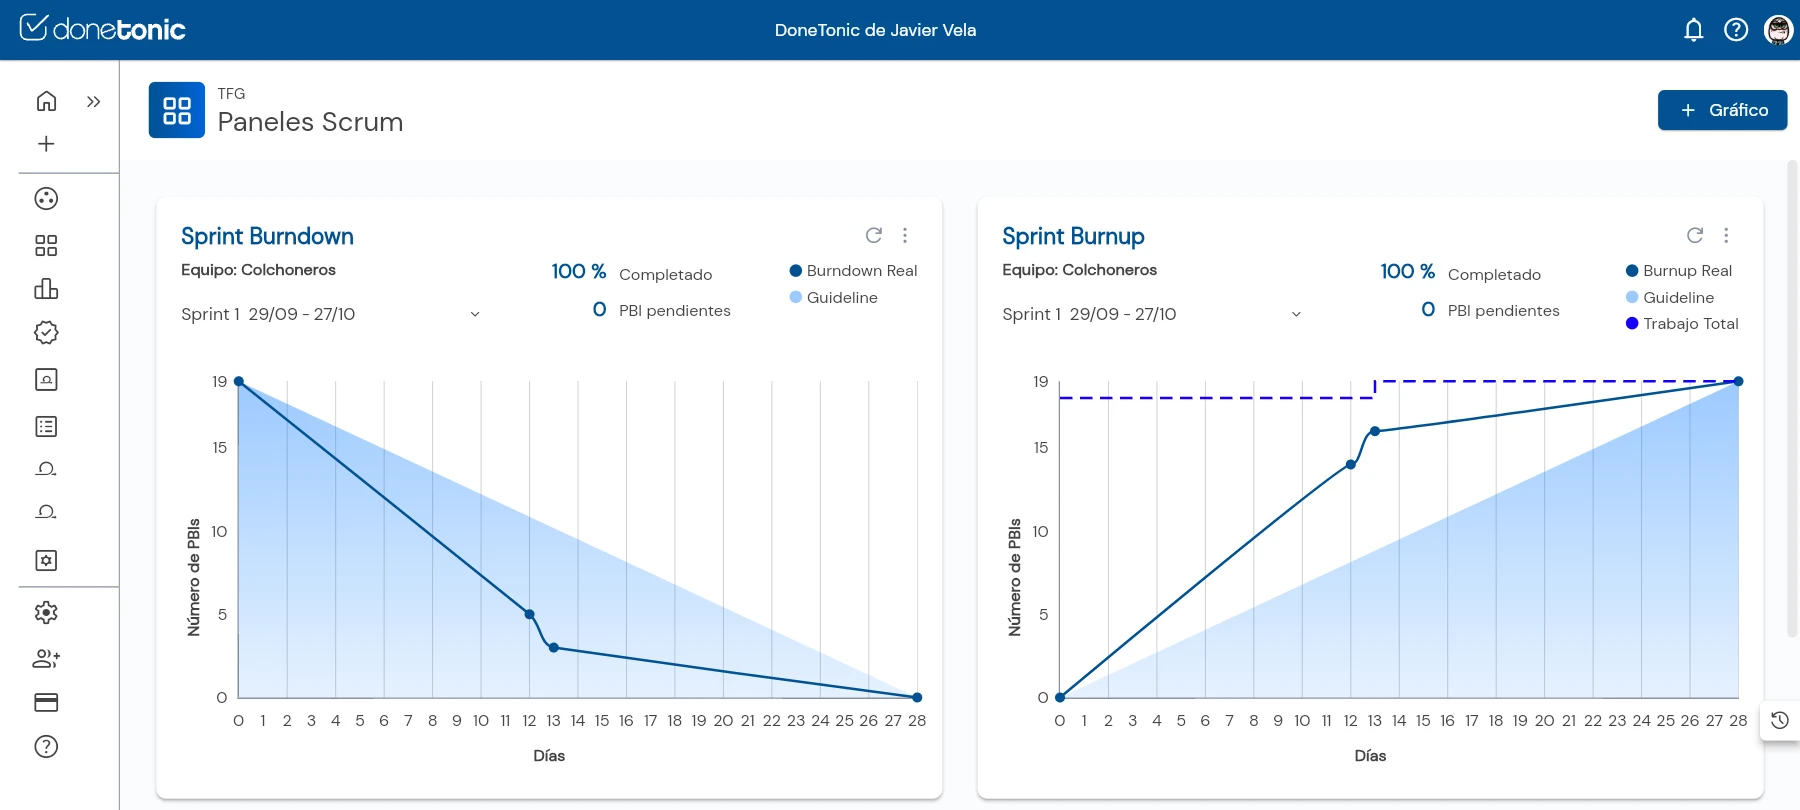
\includegraphics[width=0.9\textwidth]{figs/capturas/donetonic/02-graficas-sprint.png}
\caption{Sprint Burnup y Sprint Burndown en DoneTonic (Sprint 1).}
\label{fig:donetonic-graficas-s1}
\end{figure}

\subsubsection{Cambio de alcance}
Durante el sprint, el profesor repartió créditos de Google Cloud para educación. Para aprovecharlos se añadió el PBI \textbf{P19} (despliegue continuo en Google Cloud Run) con sus tareas T29 y T30. Render se mantuvo como despliegue alternativo. Este cambio se refleja en el burndown como un incremento temporal de PBIs pendientes (de 1 a 2) antes del cierre final.

\subsubsection{Lo aprendido}
\begin{itemize}
    \item La disciplina de GitHub Flow (rama por tarea, PR, CI obligatorio) garantiza que no se integra código roto, pero exige sincronización continua de ramas locales para evitar conflictos de avance rápido.
    \item El patrón repositorio con inyección de dependencias permitió sustituir el almacenamiento en memoria por PostgreSQL sin modificar una sola línea de la capa de lógica, respaldado por pruebas de contrato idénticas.
    \item La auditoría manual frase a frase frente al enunciado oficial demostró ser indispensable, localizando discrepancias de acceso que habían pasado inadvertidas en la formulación de los PBIs.
    \item La concentración cronológica de commits en una jornada (12/10/2026) preserva la trazabilidad estructural del proceso, si bien se reconoce la conveniencia pedagógica de una cadencia temporal más distribuida.
    \item Todo secreto compartido involuntariamente en canales de comunicación debe ser rotado como buena práctica de seguridad.
\end{itemize}

\section{Sprint 2 (Lógica del juego)}

\subsection{Planificación del Sprint 2}

\subsubsection{Objetivo y fechas}
El Sprint 2 se planificó del 23/10/2026 al 29/10/2026, tras el cierre del Sprint 1, cuando el profesor fijó que el Sprint 2 sería la lógica del juego. El juego ya estaba desarrollado en seis fases (23/10–26/10), por lo que el sprint recoge ese trabajo como backlog: 29 PBIs (P20–P48) y 50 tareas (T33–T82), con una etiqueta por fase (gestion/README.md §4.4).

\subsubsection{Sprint Backlog}
La Tabla \ref{tab:sprint2-backlog} resume los PBIs del Sprint 2 con su etiqueta, título, tareas, PRs y fecha de finalización (hecho = día fusión último PR del PBI).

{\small
\begin{longtable}{@{}L{0.7cm} L{2.2cm} L{5.5cm} L{1.5cm} L{2.0cm} L{1.8cm} L{1.5cm}@{}}
\caption{Sprint Backlog del Sprint 2 (29 PBIs, 50 tareas).}\label{tab:sprint2-backlog}\\
\toprule
\textbf{PBI} & \textbf{Etiqueta} & \textbf{Título} & \textbf{Tareas} & \textbf{PRs} & \textbf{Hecho} & \textbf{Estado} \\ \midrule \endfirsthead
\toprule
\textbf{PBI} & \textbf{Etiqueta} & \textbf{Título} & \textbf{Tareas} & \textbf{PRs} & \textbf{Hecho} & \textbf{Estado} \\ \midrule \endhead
P20 & Base del juego & Rediseño interfaz web y menú juego & T33, T34 & \#36, \#45 & 24/10/2026 & Hecho \\
P21 & Base del juego & Motor partida survivor & T35, T36 & \#36 & 23/10/2026 & Hecho \\
P22 & Base del juego & Gráficos pixel art y cámara 3/4 & T37, T38 & \#44, \#46 & 24/10/2026 & Hecho \\
P23 & Base del juego & Jugadores, entrenadores y Vestuario & T39–T41 & \#44, \#48 & 24/10/2026 & Hecho \\
P24 & Base del juego & Armas, habilidades y mejoras & T42, T43 & \#36, \#48 & 24/10/2026 & Hecho \\
P25 & Base del juego & Rivales con comportamiento propio & T44, T45 & \#44, \#45, \#47 & 24/10/2026 & Hecho \\
P26 & Base del juego & Jefes con fases & T46, T47 & \#45, \#48 & 24/10/2026 & Hecho \\
P27 & Base del juego & Mapa con terreno y obstáculos & T48, T49 & \#45, \#47 & 24/10/2026 & Hecho \\
P28 & Base del juego & Controles, pantalla completa y ajustes & T50, T51 & \#36, \#47 & 24/10/2026 & Hecho \\
P29 & Fase 2 Club & Progreso juego guardado en servidor & T52, T53 & \#49 & 24/10/2026 & Hecho \\
P30 & Fase 2 Club & Contratos: fichar jugadores & T54 & \#49 & 24/10/2026 & Hecho \\
P31 & Fase 2 Club & Entrenamiento de jugadores & T55 & \#49, \#50 & 24/10/2026 & Hecho \\
P32 & Fase 2 Club & Ranking de la grada & T56 & \#49 & 24/10/2026 & Hecho \\
P33 & Fase 3 Ultras & Combinaciones y ULTRAS & T57, T58 & \#50 & 24/10/2026 & Hecho \\
P34 & Fase 3 Ultras & Dificultad equilibrada y modo pruebas & T59, T60 & \#50 & 24/10/2026 & Hecho \\
P35 & Fase 4 Mundo & Mundo procedural natural & T61 & \#52 & 24/10/2026 & Hecho \\
P36 & Fase 4 Mundo & Ambientes por finales & T62 & \#52 & 24/10/2026 & Hecho \\
P37 & Fase 4 Mundo & Mote y avatar & T63 & \#52 & 24/10/2026 & Hecho \\
P38 & Fase 5 Rarezas & Rarezas por historia rojiblanca y fichajes & T64, T65 & \#53 & 26/10/2026 & Hecho \\
P39 & Fase 5 Rarezas & Habilidades niveladas por minuto & T66 & \#53 & 26/10/2026 & Hecho \\
P40 & Fase 5 Rarezas & Combinaciones y ultras a la vista & T67 & \#53 & 26/10/2026 & Hecho \\
P41 & Fase 5 Rarezas & Colisiones exactas & T68 & \#53 & 26/10/2026 & Hecho \\
P42 & Fase 6 Logros y sonido & Logros con historia y equipaciones & T69, T70 & \#54 & 26/10/2026 & Hecho \\
P43 & Fase 6 Logros y sonido & Pantalla fin con estadísticas & T71 & \#54 & 26/10/2026 & Hecho \\
P44 & Fase 6 Logros y sonido & Música chiptune y grada & T72–T74 & \#54 & 26/10/2026 & Hecho \\
P45 & Fase 6 Logros y sonido & Muñecos con más detalle & T75 & \#54 & 26/10/2026 & Hecho \\
P46 & Fase 6 Logros y sonido & Jefes más duros & T76 & \#54 & 26/10/2026 & Hecho \\
P47 & Calidad & Corrección errores detectados & T77–T79 & \#51, \#55, \#56 & 29/10/2026 & Hecho \\
P48 & Calidad & Documentación y gestión Sprint 2 & T80–T82 & \#55 & 29/10/2026 & Hecho \\
\bottomrule
\end{longtable}
}

La Tabla \ref{tab:sprint2-backlog} muestra el desglose completo.

\subsubsection{Historias de usuario y criterios de aceptación (Sprint 2)}
Cada PBI del Sprint 2 tiene en DoneTonic su historia de usuario y criterios de aceptación (gestion/README.md, sección «Historias de usuario y criterios de aceptación»). La Tabla \ref{tab:sprint2-hu} resume las 29 historias con sus criterios principales.

{\small
\begin{longtable}{@{}L{0.7cm} L{13.5cm}@{}}
\caption{Historias de usuario Sprint 2 (resumen).}\label{tab:sprint2-hu}\\
\toprule
\textbf{PBI} & \textbf{Historia de usuario y criterios clave} \\ \midrule \endfirsthead
\toprule
\textbf{PBI} & \textbf{Historia de usuario y criterios clave} \\ \midrule \endhead
P20 & Como aficionado quiero una web con aspecto de juego, clara en móvil y ordenador, para que entrar a jugar sea lo primero que vea al iniciar sesión. Criterios: sistema de diseño propio, modo oscuro rojiblanco, responsive, menú de juego como inicio con sesión. \\
P21 & Como jugador quiero una partida de supervivencia contra oleadas infinitas, armas automáticas y elección de mejoras al subir de nivel. Criterios: simulación determinista paso fijo 1/60 s, oleadas cada 30 s, experiencia, 3 mejoras aleatorias, dificultad creciente, pausa y fin de partida. \\
P22 & Como jugador quiero estilo visual propio con muñecos chibi del Atleti generados por código. Criterios: muñecos 16×20 px en canvas, caché de fotogramas, cámara 3/4 con inercia, respeta prefers-reduced-motion. \\
P23 & Como jugador quiero elegir entre 36 futbolistas por posición y 2 entrenadores con ulti. Criterios: stats base por posición, rasgos y habilidades propias por jugador, 2 entrenadores con bonus y ulti, Vestuario con filtro y ficha. \\
P24 & Como jugador quiero 24 armas/habilidades con 5 niveles, pasivas y mejoras extra. Criterios: armas disparo y melé, 5 niveles, pasivas, mejoras extra sin límite, porteros sin armas de disparo. \\
P25 & Como jugador quiero 16 equipos rivales con comportamientos variados. Criterios: 16 equipos desbloqueables por oleadas, arquetipos embestida/disparo, rodean obstáculos, élites blindado/veloz/furioso. \\
P26 & Como jugador quiero 10 jefes con 3 fases, avisos, escolta y jugada estrella. Criterios: jefe cada 4 oleadas, 3 fases (66\%, 33\%), escolta desde 2º jefe, furia por tiempo, jugada estrella en fase 3. \\
P27 & Como jugador quiero mapa procedural con biomas, barro, lluvia, gradas, mesetas. Criterios: ruido armónico continuo, distritos, gradas orientadas, plazas, barro/lluvia, mesetas con escaleras, casi todo alcanzable. \\
P28 & Como jugador quiero controles teclado, ratón, táctil, pausa, pantalla completa, ajustes. Criterios: WASD/flechas, joystick táctil, F pantalla completa, Esc/P pausa, ajustes guardados en navegador. \\
P29 & Como jugador quiero mi club y partidas guardados en mi cuenta con validación anti-trampas. Criterios: tablas juego\_perfiles y juego\_records, API /api/juego protegida, validación servidor con reloj propio y límites creíbles, concurrencia optimista. \\
P30 & Como jugador quiero ganar fichas de contrato venciendo jefes y canjearlas por jugadores. Criterios: plantilla inicial 4 comunes, 1 ficha por 3 jefes, sorteo ponderado por rareza, sin repetir jugador. \\
P31 & Como jugador quiero entrenar a mis jugadores con puntos de jefes y bajas. Criterios: puntos por jefes (1 cada 3) y bajas (coste creciente), 4 stats (Vida, Defensa, Disparo, Suerte) máx. 20, validado en servidor. \\
P32 & Como jugador quiero ranking global con la mejor marca de cada aficionado sin mostrar correo. Criterios: una fila por usuario (mejor tiempo, desempate nivel), pestañas Mis partidas / La grada, anonimizado. \\
P33 & Como jugador quiero 24 combinaciones tácticas y 6 ULTRAS automáticas al completar combinaciones. Criterios: 24 sinergias con bonus, 6 ULTRAS (Puskás, Balón de Oro, MVP Champions, Zamora, Bota de Oro, Mejor Mundial), efecto visual y daño porcentual reducido vs jefes. \\
P34 & Como jugador quiero dificultad justa y modo pruebas para admin. Criterios: tramo final duro desde min 9, rivales curtidos min 12, ayuda inicial 8 min, modo pruebas admin (desbloqueo sin tocar ranking). \\
P35 & Como jugador quiero mundo procedural natural con distritos, estadios, plazas, mesetas. Criterios: ruidos suaves continuos, gradas orientadas, plazas con tiendas, mesetas con escaleras, casi todo alcanzable (test). \\
P36 & Como jugador quiero 5 ambientes que cambien cada 5 min (pretemporada → Copa → Liga → Champions → Mundial). Criterios: cambio de luz, césped, afición, carteles, rivales más fuertes, camisetas de selección en Mundial. \\
P37 & Como jugador quiero mote único y avatar propio en cabecera y ranking. Criterios: mote 3-16 chars único normalizado (sin mayúsculas/tildes), avatar de jugador/entrenador fichado, migración 004, PUT /api/juego/identidad. \\
P38 & Como aficionado quiero rarezas según historia rojiblanca y animación de firma al fichar. Criterios: 4 rarezas (Común 12, Raro 8, Épico 8, Leyenda 8) por historia en el club, más rareza = más habilidades y menos probabilidad, animación firma pixel art. \\
P39 & Como jugador quiero que habilidades fuertes no salgan al principio. Criterios: niveles bloqueados por minuto (desdeMinuto) y recarga mínima (cdMin), regate/entrada/contragolpe reequilibrados. \\
P40 & Como jugador quiero ver combinaciones y ULTRAS con filtros. Criterios: pantalla Combinaciones con nombre, bonus, requisitos, ultra asociada, filtros Todas/Con tu jugador/Conseguidas. \\
P41 & Como jugador quiero colisiones exactas (lo que se ve choca). Criterios: hitbox por los pies (vista 3/4), obstáculos macizos en todo su dibujo, copa de árboles transparente. \\
P42 & Como aficionado quiero 29 logros con datos históricos que desbloqueen 10 equipaciones. Criterios: 29 logros con dato real, servidor valida los comprobables, 10 equipaciones en Vestuario. \\
P43 & Como jugador quiero pantalla de fin con desglose de daño por arma y recompensas. Criterios: tiempo, ambiente, bajas, jefes, daño total, golpe máx, críticos, daño recibido, vida recuperada, barras por arma/ultra/ulti/quemaduras, logros nuevos. \\
P44 & Como jugador quiero música chiptune, fanfarrias y grada con volumen independiente. Criterios: secuenciador chiptune propio, canción por ambiente que anima con tiempo/jefes, fanfarria por competición, grada con murmullo/cánticos según distancia, todo Web Audio sin archivos. \\
P45 & Como aficionado quiero reconocer jugadores y jefes en el campo. Criterios: sombreado, orejas, nariz, peinados, rasgos propios (brazalete, cinta, pecas, barba, pendientes, tatuajes). \\
P46 & Como jugador quiero jefes más duros a partir del segundo. Criterios: escolta de élites desde 2º jefe, refuerzos al cambiar fase, furia si tardas, jugada estrella en fase 3, 1º jefe asequible. \\
P47 & Como usuario quiero que los errores encontrados se arreglen con pruebas de regresión. Criterios: cada error reproducido con prueba antes de arreglar, arreglos pasan CI y se despliegan. \\
P48 & Como responsable quiero todo el Sprint 2 revisable desde el repo. Criterios: README con capturas juego y DoneTonic, documentación técnica para memoria, backlog/tablero/gráficas Sprint 2 en DoneTonic. \\
\bottomrule
\end{longtable}
}

La Tabla \ref{tab:sprint2-hu} condensa las 29 historias de usuario del Sprint 2.

\subsubsection{Trazabilidad}
Las tareas de cada PBI indican en su descripción de DoneTonic el PR donde está el trabajo. La Tabla \ref{tab:sprint2-trazabilidad} muestra la correspondencia tarea → PR.

{\small
\begin{longtable}{@{}L{0.7cm} L{1.0cm} L{5.5cm} L{3.0cm} L{2.5cm}@{}}
\caption{Trazabilidad tarea → PR del Sprint 2 (50 tareas).}\label{tab:sprint2-trazabilidad}\\
\toprule
\textbf{PBI} & \textbf{Tarea} & \textbf{Descripción} & \textbf{PR} & \textbf{Estado} \\ \midrule \endfirsthead
\toprule
\textbf{PBI} & \textbf{Tarea} & \textbf{Descripción} & \textbf{PR} & \textbf{Estado} \\ \midrule \endhead
P20 & T33 & Sistema de diseño: tokens, tipografía y modo oscuro rojiblanco & \#36 & Hecho \\
P20 & T34 & Menú del juego como inicio con sesión (hub con jugador paseando) & \#36, \#45 & Hecho \\
P21 & T35 & Simulación de paso fijo con semilla (mundo.js) & \#36 & Hecho \\
P21 & T36 & Oleadas, experiencia y mejoras al subir de nivel & \#36 & Hecho \\
P22 & T37 & Muñecos chibi generados por código (sprites.js) & \#44 & Hecho \\
P22 & T38 & Cámara 3/4, inercia y sensación de movimiento y golpes & \#46 & Hecho \\
P23 & T39 & Jugadores con estadísticas por posición y habilidades propias & \#44, \#48 & Hecho \\
P23 & T40 & Entrenadores con ulti y pantalla Dirección & \#44 & Hecho \\
P23 & T41 & Vestuario renovado con filtros y ficha & \#48 & Hecho \\
P24 & T42 & Armas con 5 niveles: disparo, cuerpo a cuerpo y movilidad & \#36, \#48 & Hecho \\
P24 & T43 & Pasivas y mejoras extra & \#36 & Hecho \\
P25 & T44 & 16 equipos rivales que se desbloquean por oleadas & \#44 & Hecho \\
P25 & T45 & Rivales que embisten, disparan y rodean obstáculos & \#45, \#47 & Hecho \\
P26 & T46 & Jefes con tres fases y avisos de ataque & \#45 & Hecho \\
P26 & T47 & Seis jefes nuevos con habilidades propias & \#48 & Hecho \\
P27 & T48 & Barro, lluvia, gradas y premios & \#45 & Hecho \\
P27 & T49 & Mapa procedural con biomas y estructuras & \#47 & Hecho \\
P28 & T50 & Entrada por teclado y joystick táctil & \#36 & Hecho \\
P28 & T51 & Pantalla completa, pausa y ajustes en partida & \#47 & Hecho \\
P29 & T52 & Migración 003 y repositorios del juego (memoria y PostgreSQL) & \#49 & Hecho \\
P29 & T53 & API del juego con validación anti-trampas & \#49 & Hecho \\
P30 & T54 & Fichas por jefes y sorteo de contratos por rareza & \#49 & Hecho \\
P31 & T55 & Puntos y estadísticas de entrenamiento & \#49, \#50 & Hecho \\
P32 & T56 & Ranking multijugador con la mejor partida de cada usuario & \#49 & Hecho \\
P33 & T57 & Combinaciones con nombre y bonus & \#50 & Hecho \\
P33 & T58 & Seis ULTRAS con efectos visuales & \#50 & Hecho \\
P34 & T59 & Curvas de dificultad calibradas con un bot & \#50 & Hecho \\
P34 & T60 & Modo pruebas para administradores & \#50 & Hecho \\
P35 & T61 & Generación del terreno por ruidos (terreno.js) & \#52 & Hecho \\
P36 & T62 & Cinco ambientes con cambio de luz, afición y fuerza & \#52 & Hecho \\
P37 & T63 & Migración 004, API de identidad y pantalla Tu ficha & \#52 & Hecho \\
P38 & T64 & Rarezas por historia y 36 jugadores & \#53 & Hecho \\
P38 & T65 & Animación de la firma del contrato & \#53 & Hecho \\
P39 & T66 & Niveles bloqueados por minuto y recarga mínima & \#53 & Hecho \\
P40 & T67 & Pantalla de combinaciones y ultras con filtros & \#53 & Hecho \\
P41 & T68 & Hitbox por los pies y obstáculos macizos & \#53 & Hecho \\
P42 & T69 & Logros validados en el servidor (logros.js) & \#54 & Hecho \\
P42 & T70 & Pantalla Logros y equipaciones en el Vestuario & \#54 & Hecho \\
P43 & T71 & Atribución del daño por fuente y pantalla de fin (fin-ui.js) & \#54 & Hecho \\
P44 & T72 & Secuenciador chiptune y fanfarrias (musica.js) & \#54 & Hecho \\
P44 & T73 & La grada: murmullo y cánticos según la cercanía & \#54 & Hecho \\
P44 & T74 & Efectos de sonido nuevos y ajuste de música & \#54 & Hecho \\
P45 & T75 & Rasgos y sombreado en sprites.js & \#54 & Hecho \\
P46 & T76 & Escolta, furia y jugada estrella & \#54 & Hecho \\
P47 & T77 & El juego no cargaba (variable usada antes de existir) & \#51 & Hecho \\
P47 & T78 & El primer clic en «Reenviar el correo» se perdía tras un error & \#55 & Hecho \\
P47 & T79 & No se podía volver tras eliminar la cuenta (Google) & \#56 & Hecho \\
P48 & T80 & README del Sprint 2 con capturas del juego y de DoneTonic & \#55 & Hecho \\
P48 & T81 & Documentación técnica para la memoria & \#55 & Hecho \\
P48 & T82 & Backlog y seguimiento del Sprint 2 en DoneTonic & — (DoneTonic) & Hecho \\
\bottomrule
\end{longtable}
}

La Tabla \ref{tab:sprint2-trazabilidad} detalla las 50 tareas del Sprint 2.

\subsection{Desarrollo del Sprint 2: problemas y soluciones}

Los problemas detectados durante el Sprint 2 y sus soluciones (documentacion-tecnica.md §13) se recogen en la Tabla \ref{tab:prob-sprint2}.

\begin{longtable}{@{}L{5.5cm} L{8.5cm}@{}}
\caption{Problemas y soluciones del Sprint 2.}\label{tab:prob-sprint2}\\
\toprule
\textbf{Problema detectado} & \textbf{Solución adoptada} \\ \midrule \endfirsthead
\toprule
\textbf{Problema detectado} & \textbf{Solución adoptada} \\ \midrule \endhead
El juego dejó de cargar tras un cambio (variable usada antes de existir) & Arreglo inmediato (PR \#51) y prueba que importa todos los módulos del juego \\
Jugadores podían esconderse detrás de tejados (colisión no coincidía con dibujo 3/4) & Colisión por los pies y obstáculos macizos en todo su dibujo (PR \#53) \\
Tirones al pintar el suelo (muchas texturas por píxel en mismo fotograma) & Una textura por celda y ambiente, como mucho una por fotograma y por adelantado (PR \#52) \\
Simulación lenta con muchos rivales (búsqueda claves texto) & Búsqueda por radio con claves numéricas empaquetadas: 4,5× más rápido (PR \#52) \\
Regate hacía al jugador intocable demasiado pronto (subía sin límite) & Niveles bloqueados por minuto (desdeMinuto) y recarga mínima (cdMin) (PR \#53) \\
Equilibrio difícil de ajustar a mano (muchas variables) & Todo el equilibrio en config.js y calibración con bot que juega partidas simuladas (PR \#50) \\
Eliminar cuenta (especialmente Google) impedía volver a entrar con ese email & Migración 005: índice parcial unique en email (solo cuentas no eliminadas), findByEmail ignora eliminadas, suelta mote y sale del ranking (PR \#56) \\
Primer clic en «Reenviar el correo» se perdía tras error de login & Campo vacío sin tocar no da error al salir; tras fallo servidor se vacía contraseña sin marcar error (PR \#55) \\
\bottomrule
\end{longtable}

La Tabla \ref{tab:prob-sprint2} resume los 8 problemas principales del Sprint 2.

\subsection{Revisión del Sprint 2}

Al cierre del Sprint 2 (29/10/2026) se entregaron:
\begin{itemize}
    \item 29 PBIs completados (P20–P48).
    \item 50 tareas cerradas (T33–T82).
    \item 14 PRs fusionados (\#36, \#44–\#56).
    \item Batería de 276 pruebas automatizadas (136 del juego) validadas en CI contra PostgreSQL 17.
    \item Documentación técnica actualizada (documentacion-tecnica.md) y README con capturas del juego y DoneTonic.
    \item Backlog, tablero y gráficas del Sprint 2 registrados en DoneTonic.
\end{itemize}

\subsection{Retrospectiva del Sprint 2}

\subsubsection{Burndown real del Sprint 2}
La Figura \ref{fig:burndown-s2} muestra la evolución real de PBIs pendientes según la fecha de fusión del último PR de cada PBI (tabla «Evolución del Sprint 2» en gestion/README.md). A diferencia de las gráficas de DoneTonic (que salen en recta porque el backlog se registró al cerrar el sprint el 29/10), este burndown refleja el trabajo real día a día.

\begin{figure}[htbp]
\centering
\begin{tikzpicture}
\begin{axis}[
    width=0.9\textwidth,
    height=7cm,
    xlabel={Fecha},
    ylabel={PBIs pendientes},
    xtick={1,2,3,4,5,6,7},
    xticklabels={23/10, 24/10, 25/10, 26/10, 27/10, 28/10, 29/10},
    ymin=0, ymax=29,
    grid=major,
    legend pos=north east,
    mark=*,
    thick
]
\addplot coordinates {(1,28) (2,11) (3,11) (4,2) (5,2) (6,2) (7,0)};
\addlegendentry{PBIs pendientes}
\end{axis}
\end{tikzpicture}
\caption{Burndown real del Sprint 2 (PBIs pendientes según fechas de PR).}
\label{fig:burndown-s2}
\end{figure}

\subsubsection{Seguimiento visual en DoneTonic}
Las Figuras \ref{fig:donetonic-tablero-s2}, \ref{fig:donetonic-graficas-s2} y \ref{fig:donetonic-backlog} muestran el tablero, las gráficas Sprint Burndown/Burnup y el Backlog Burndown/Burnup del Sprint 2 en DoneTonic (capturas 04, 06 y 07 de donetonic).

\begin{figure}[htbp]
\centering
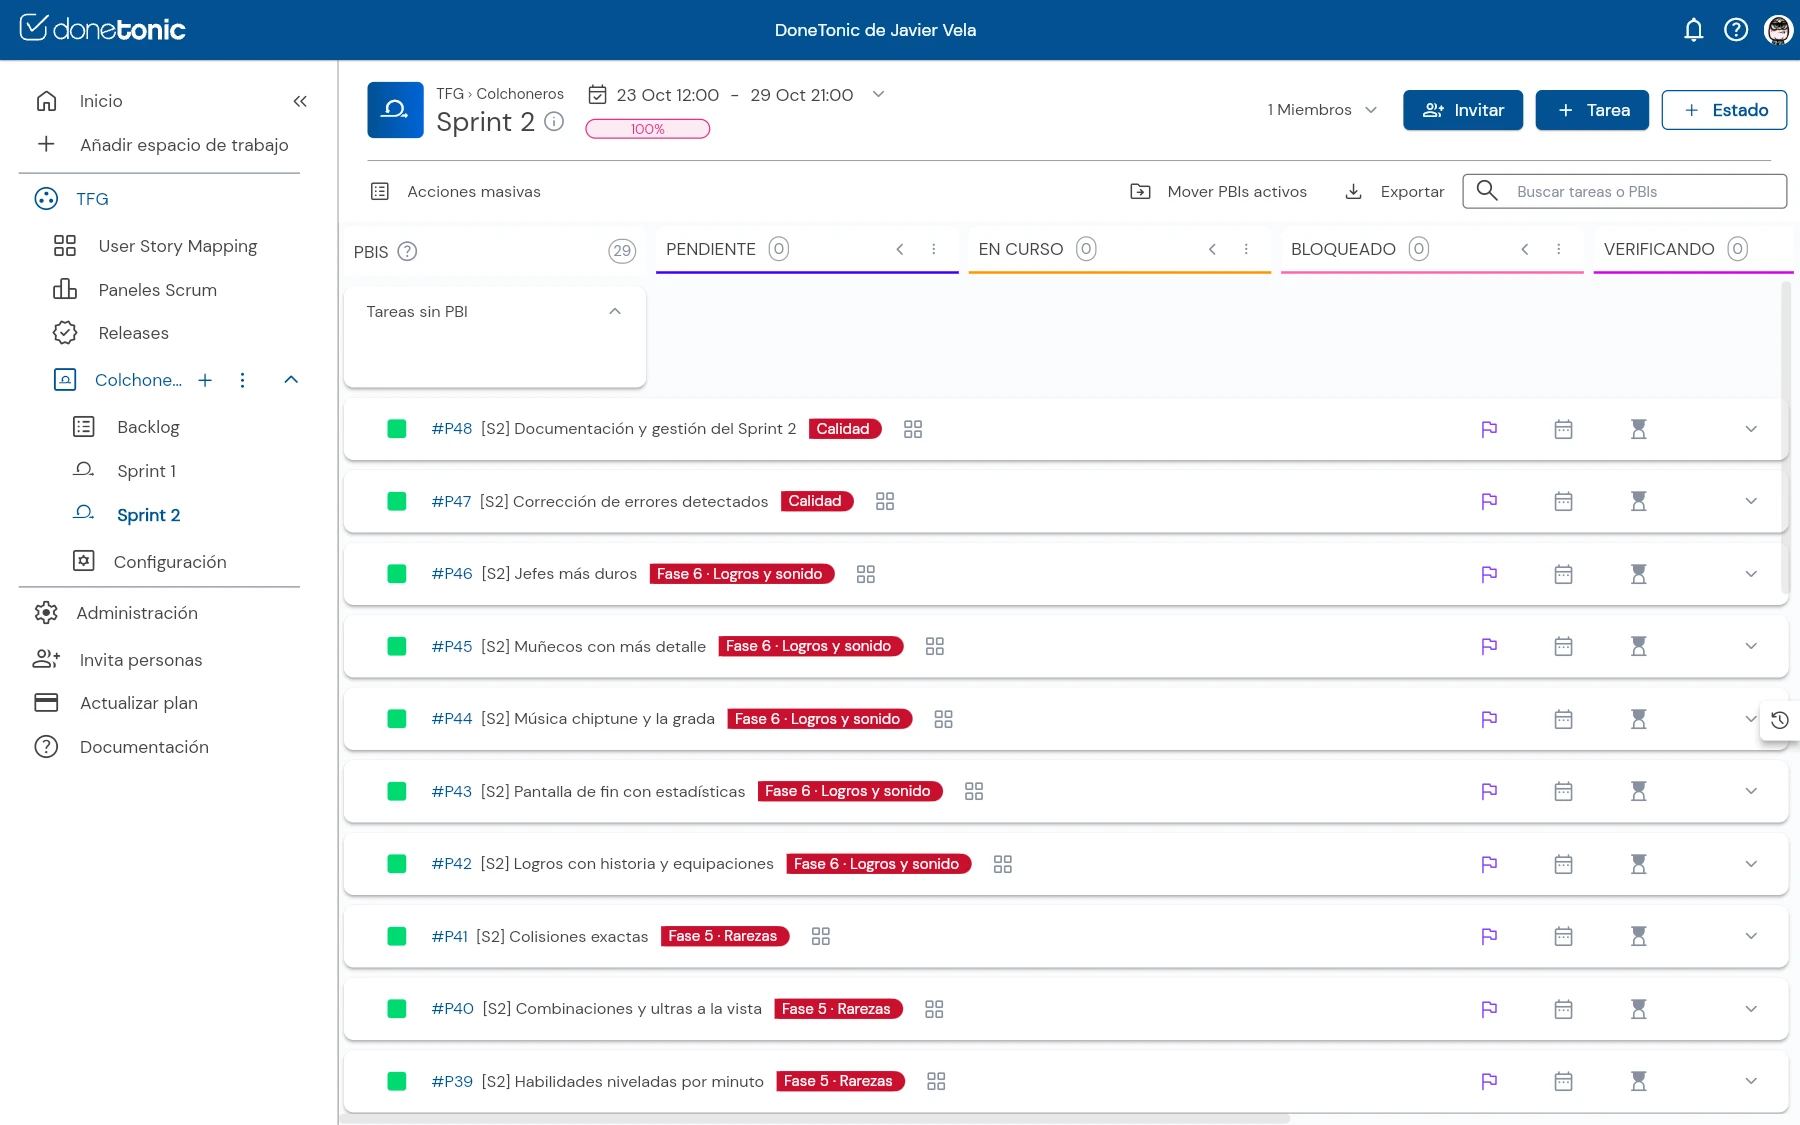
\includegraphics[width=0.9\textwidth]{figs/capturas/donetonic/04-tablero-sprint2.png}
\caption{Tablero del Sprint 2 en DoneTonic al 100\%.}
\label{fig:donetonic-tablero-s2}
\end{figure}

\begin{figure}[htbp]
\centering
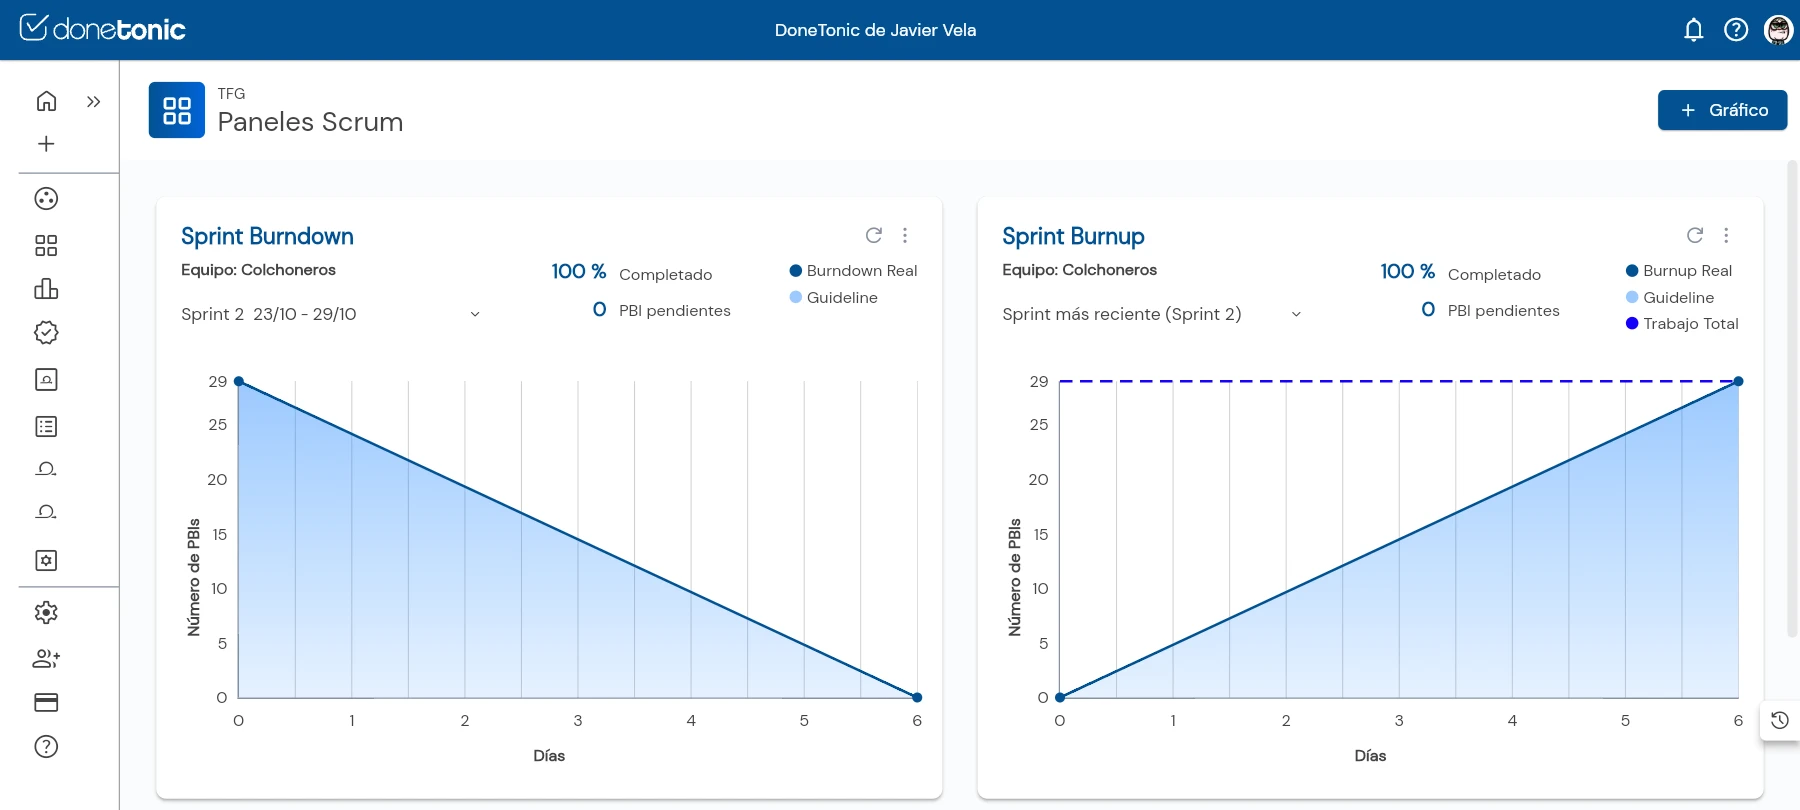
\includegraphics[width=0.9\textwidth]{figs/capturas/donetonic/06-graficas-sprint2.png}
\caption{Sprint Burndown y Burnup del Sprint 2 en DoneTonic (aplanadas por registro tardío).}
\label{fig:donetonic-graficas-s2}
\end{figure}

\begin{figure}[htbp]
\centering
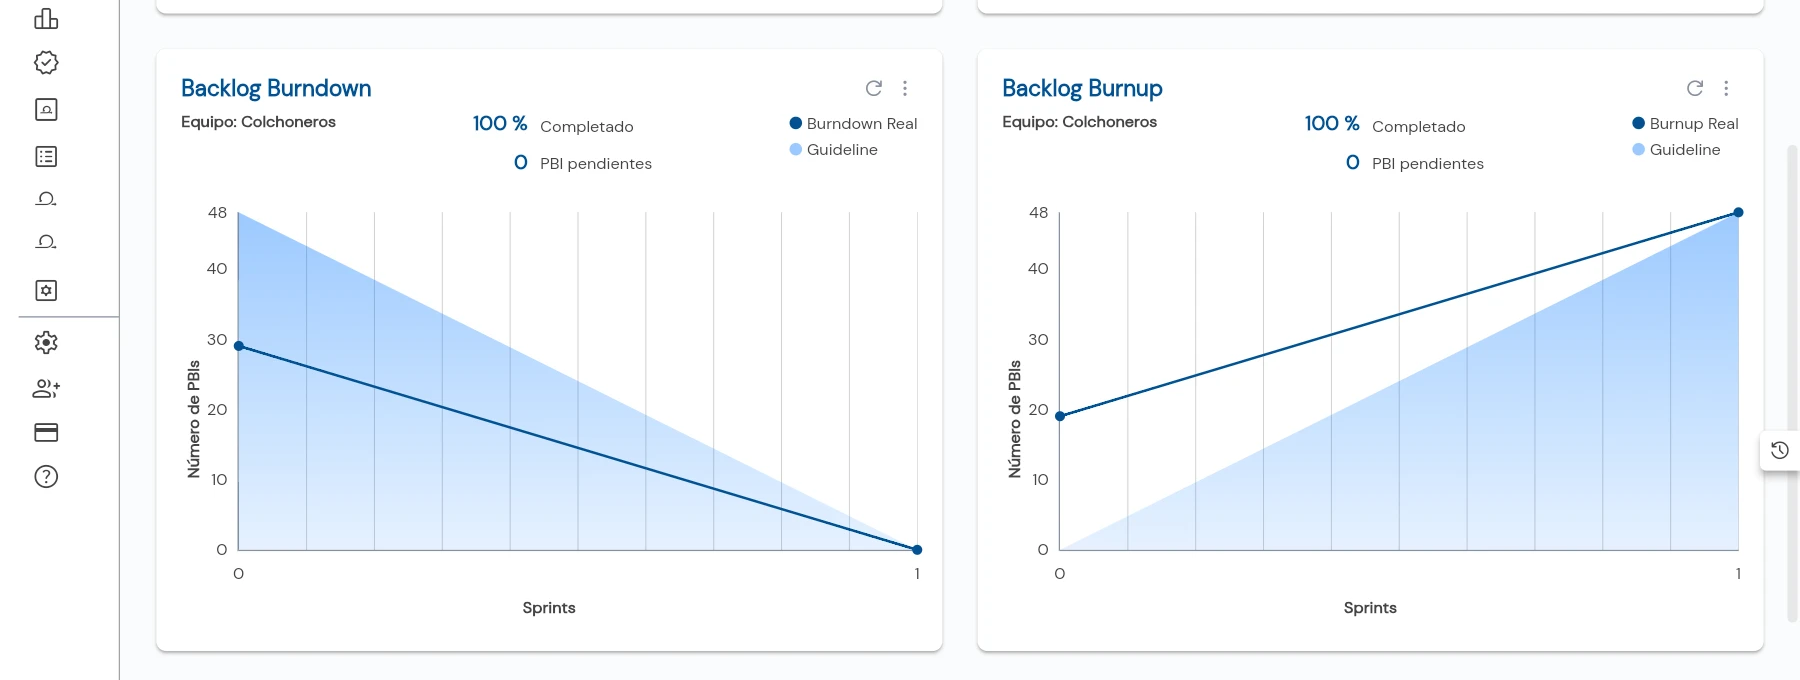
\includegraphics[width=0.9\textwidth]{figs/capturas/donetonic/07-graficas-backlog.png}
\caption{Backlog Burndown y Burnup de los dos sprints en DoneTonic.}
\label{fig:donetonic-backlog}
\end{figure}

\subsubsection{Explicación de las gráficas planas en DoneTonic}
Como se indica en la Figura \ref{fig:donetonic-graficas-s2}, las gráficas de DoneTonic del Sprint 2 aparecen como una recta porque el backlog completo (29 PBIs, 50 tareas) se registró en la herramienta el 29/10/2026, al cerrar el sprint, marcando todos los PBIs como hechos ese mismo día. La evolución real del trabajo (del 23 al 26/10) se reconstruye a partir de las fechas de fusión de los PRs, como se muestra en la Figura \ref{fig:burndown-s2}.

\subsubsection{Lo aprendido}
\begin{itemize}
    \item La arquitectura en capas y la inyección de dependencias permitieron añadir la lógica del juego (11.000 líneas) sin tocar la base SaaS, reutilizando usuarios, sesiones, roles, persistencia y CI/CD.
    \item La simulación determinista con paso fijo y semilla facilitó las pruebas automáticas del motor (136 pruebas) y la validación anti-trampas en el servidor.
    \item La generación procedural de gráficos y audio por código eliminó dependencias de assets externos y permitió variaciones dinámicas (equipaciones, selecciones, intensidad musical).
    \item La concurrencia optimista (columna \texttt{version} en \texttt{juego\_perfiles}) resolvió condiciones de carrera al fichar/entrenar sin bloqueos pesados.
    \item El registro tardío en DoneTonic distorsiona las métricas visuales; para retrospectivas reales hay que cruzar con fechas de PR/commits.
\end{itemize}

\chapter{Material Adicional}
\label{anx:material}

\section{Enlaces del proyecto}

\begin{sloppypar}
\setlength{\emergencystretch}{5em}
\begin{itemize}
    \item \textbf{Repositorio principal:}\\
    \url{https://github.com/VelaElDios/la-grada-colchonera-saas}
    \item \textbf{Aplicación desplegada (Google Cloud Run):}\\
    \url{https://la-grada-colchonera-1081564062572.europe-southwest1.run.app}
    \item \textbf{Releases publicadas} (\texttt{hito-1}, \texttt{hito-2}, \texttt{hito-3}, \texttt{hito-4} y \texttt{sprint-1}):\\
    \url{https://github.com/VelaElDios/la-grada-colchonera-saas/releases}
    \item \textbf{Documentación del repositorio:}
    \begin{itemize}
        \item \texttt{README.md}: visión general, tecnologías, ejecución local, pruebas, variables de entorno, API, despliegue y acceso como administrador.
        \item \texttt{CONTRIBUTING.md}: flujo de trabajo con ramas, commits y pull requests.
        \item \texttt{docs/revision-entrega.md}: revisión frase a frase del enunciado con su evidencia.
        \item \texttt{docs/gestion/README.md}: backlog de los dos sprints, trazabilidad tarea $\rightarrow$ rama $\rightarrow$ PR y capturas de DoneTonic.
        \item \texttt{docs/documentacion-tecnica.md}: documentación técnica completa (requisitos, arquitectura, flujos, seguridad, juego, pruebas, CI/CD, métricas).
        \item \texttt{docs/hito4-configuracion.md}: configuración del correo (SMTP) y del cliente OAuth de Google.
    \end{itemize}
    \item \textbf{Gestión del proyecto (DoneTonic)}, espacio de trabajo \textit{TFG}, equipo \textit{Colchoneros}:\\
    \url{https://app.donetonic.com}
\end{itemize}
\end{sloppypar}

\section{Credenciales de administrador para la revisión}
Las credenciales del primer administrador (valores de \texttt{ADMIN\_EMAIL} y \texttt{ADMIN\_PASSWORD}) se envían junto con la entrega, tal como se indica en el \texttt{README.md} (sección «Acceso como administrador para la revisión»). No están en el repositorio ni en esta memoria.

\chapter{Uso Responsable de la Inteligencia Artificial}
\label{anx:ia}

De acuerdo con las directrices académicas sobre honestidad y rigor en la autoría de trabajos universitarios, este anexo documenta con absoluta transparencia el uso de asistentes basados en modelos de inteligencia artificial a lo largo de las distintas etapas del proyecto.

\section{Uso de la inteligencia artificial en el desarrollo del software}

Durante la ejecución técnica del Sprint 1 se utilizó el modelo Claude (Cowork) como asistente de desarrollo para agilizar las tareas de implementación. Su papel abarcó la redacción del código fuente en JavaScript, la preparación de ficheros de configuración, la elaboración de la documentación técnica y la generación de los mensajes de confirmación de cambios. Dichos commits quedaron registrados con la autoría formal del alumno y el correspondiente metadato de colaboración (\texttt{Co-Authored-By}). Asimismo, el asistente gestionó en el navegador la apertura y fusión de los pull requests y la actualización de los estados en el tablero ágil de DoneTonic.

No obstante, el control del entorno productivo y la gobernanza del proyecto recayeron en todo momento en el alumno:
\begin{itemize}
    \item La creación, administración y custodia de credenciales en las plataformas de infraestructura (Neon para PostgreSQL, Render y Google Cloud Run) fueron realizadas personalmente por el alumno.
    \item El aseguramiento de la calidad técnica no se delegó en la generación sintética de la IA, sino en una suite de 80 pruebas automatizadas ejecutadas obligatoriamente en el pipeline de integración continua ante cada cambio propuesto.
    \item El alumno llevó a cabo una auditoría manual frente a las especificaciones oficiales (\texttt{docs/\allowbreak revision-\allowbreak entrega.md}), detectando y corrigiendo oportunamente una discrepancia de permisos en la comprobación de usuarios activos (PR \#30).
\end{itemize}

\section{Uso de la inteligencia artificial en la redacción de la memoria}

Para la composición de esta memoria técnica se empleó un flujo automatizado denominado «Cerebro Universal», orquestado sobre GitHub Actions y sustentado en modelos de lenguaje gratuitos. En dicho sistema, una IA constructora generó las secciones del documento y una IA revisora analizó la consistencia de cada avance.

La fidelidad de la información redactada se garantizó mediante estrictas salvaguardas metodológicas:
\begin{itemize}
    \item Los modelos operaron exclusivamente sobre la información factual contenida en la guía del proyecto y los documentos reales del repositorio, quedando descartada cualquier inferencia externa no contrastada.
    \item Un proceso de verificación algorítmica independiente comprobó que el documento compilase sin fallos, sin marcadores de relleno de plantilla, con todas las citas bibliográficas resueltas y certificando que ningún dato cuantitativo superior a 20 careciese de respaldo en las fuentes.
    \item Claude intervino en la preparación de la estructura inicial de la plantilla en LuaLaTeX, las fuentes de datos y las pruebas de comprobación sintáctica.
\end{itemize}

El alumno asume la autoría y responsabilidad íntegra sobre el contenido final expuesto en la presente memoria, habiendo revisado minuciosamente el texto para certificar su rigor técnico y su estricta correspondencia con el trabajo desarrollado.


% -------------------------------
% Bibliografía
% -------------------------------
\cleardoublepage
\bibliographystyle{apalike}
\bibliography{bib/ref}
\addcontentsline{toc}{chapter}{Referencia bibliográfica}

\end{document}
